\documentclass[a4paper,oneside,14pt]{extreport}

\usepackage[T2A]{fontenc}
\usepackage[utf8]{inputenc}
\usepackage[english,russian]{babel}

%\usepackage[left=30mm, right=20mm, top=20mm, bottom=20mm]{geometry}
\usepackage[left=20mm, right=10mm, top=5mm, bottom=20mm]{geometry}

\usepackage{microtype}
\sloppy

\usepackage{setspace}
\onehalfspacing

\usepackage{indentfirst}
\setlength{\parindent}{12.5mm}

\usepackage{titlesec}
\titleformat{\chapter}{\LARGE\bfseries}{\thechapter}{14pt}{\LARGE\bfseries}
\titlespacing*{\chapter}{\parindent}{0mm}{5mm}
\titleformat{\section}{\Large\bfseries}{\thesection}{14pt}{\Large\bfseries}

\addto{\captionsrussian}{\renewcommand*{\contentsname}{Содержание}}
\usepackage{natbib}
\renewcommand{\bibsection}{\chapter*{Список использованных источников}}

\usepackage{caption}

\usepackage{wrapfig}
\usepackage{float}

\usepackage{graphicx}
\newcommand{\imgwc}[4]
{
	\begin{figure}[#1]
		\center{\includegraphics[width=#2]{inc/img/#3}}
		\caption{#4}
		\label{img:#3}
	\end{figure}
}
\newcommand{\imghc}[4]
{
	\begin{figure}[#1]
		\center{\includegraphics[height=#2]{inc/img/#3}}
		\caption{#4}
		\label{img:#3}
	\end{figure}
}
\newcommand{\imgsc}[4]
{
	\begin{figure}[#1]
		\center{\includegraphics[scale=#2]{inc/img/#3}}
		\caption{#4}
		\label{img:#3}
	\end{figure}
}

\usepackage{pgfplots}
\pgfplotsset{compat=newest}

\usepackage{listings}
\usepackage{listingsutf8}
\lstset{
	basicstyle=\footnotesize\ttfamily,
	keywordstyle=\color{blue},
	stringstyle=\color{red},
	commentstyle=\color{gray},
	numbers=left,
	numberstyle=\tiny,
	numbersep=5pt,
	frame=false,
	breaklines=true,
	breakatwhitespace=true,
	inputencoding=utf8/koi8-r
}

\lstdefinestyle{c}{
	language=C++,
	backgroundcolor=\color{white},
	basicstyle=\footnotesize\ttfamily,
	keywordstyle=\color{blue},
	stringstyle=\color{red},
	commentstyle=\color{gray},
	directivestyle=\color{orange},
	numbers=left,
	numberstyle=\tiny,
	stepnumber=1,
	numbersep=5pt,
	frame=single,
	tabsize=4,
	captionpos=t,
	breaklines=true,
	breakatwhitespace=true,
	escapeinside={\#*}{*)},
	morecomment=[l][\color{magenta}]{\#},
	columns=fullflexible
}

\newcommand{\code}[1]{\texttt{#1}}

\usepackage{amsmath}
\usepackage{amssymb}

\usepackage[unicode]{hyperref}
\hypersetup{hidelinks}

\makeatletter
\newcommand{\vhrulefill}[1]
{
	\leavevmode\leaders\hrule\@height#1\hfill \kern\z@
}
\makeatother

\begin{document}

\begin{titlepage}
	\centering
	
	\vspace{-2.2mm}
	\vhrulefill{0.9mm}\\
	\vspace{-7mm}
	\vhrulefill{0.2mm}\\
	\vspace{2mm}
	
	\vspace{50mm}
	
	\vspace{30mm}
	
	\textbf{Отчет по лабораторной работе №7}\\
	По курсу: <<Фильтрация и прогнозирование данных>>\\
	Тема: <<Решение обратной задачи>>\\
	
	\vspace{60mm}
	
	\hspace{70mm} Студент:       \hfill Пронин~А.~С.\\
	\hspace{70mm} Группа:        \hfill МСМТ231\\
	\hspace{70mm} Преподаватель: \hfill Зотов~Л.~В.\\
	%	\hspace{70mm} Оценка:        \hfill \hrulefill\\
	
	\vfill
	
	Москва\\
	\the\year
\end{titlepage}

\setcounter{page}{2}

\chapter*{Лабораторная работа 5}

\textbf{Часть 1}

Для начала выведем наш сигнал из ЛР1 (рис. \ref{task1_signal}):
\begin{figure}[!h]
	\center{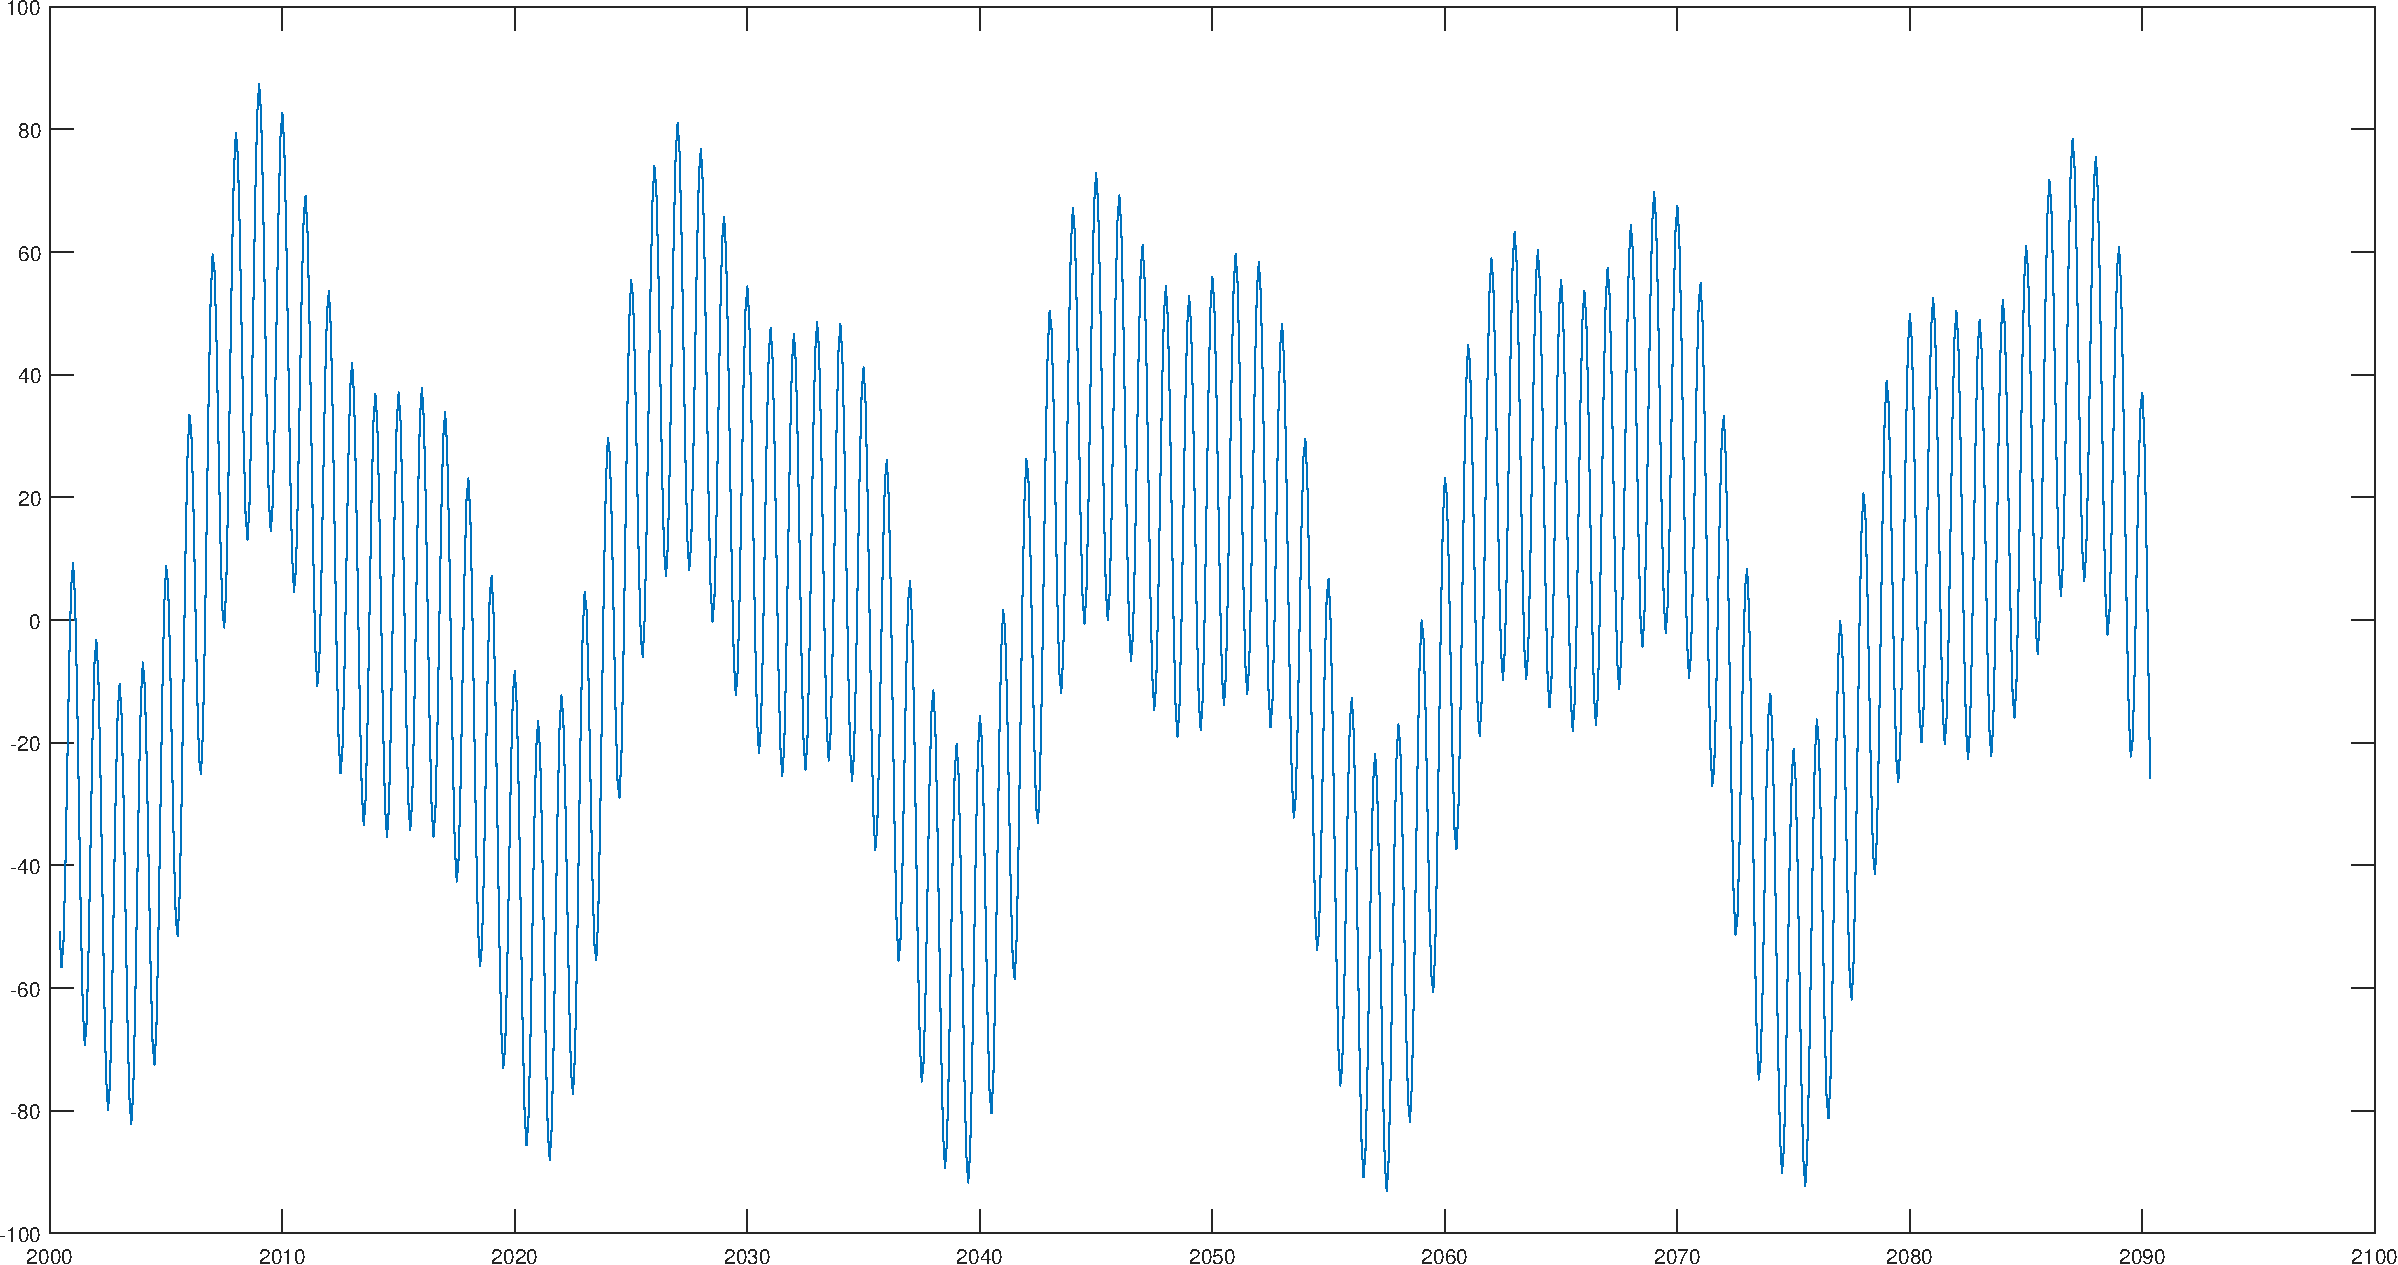
\includegraphics[width=1\linewidth]{inc/task1_signal}}
	\caption{Сигнал из ЛР1}
	\label{task1_signal}
\end{figure}

Затем сгенерируем авто-регрессионный шум (рис. \ref{task1_noise}):
\begin{figure}[!h]
	\center{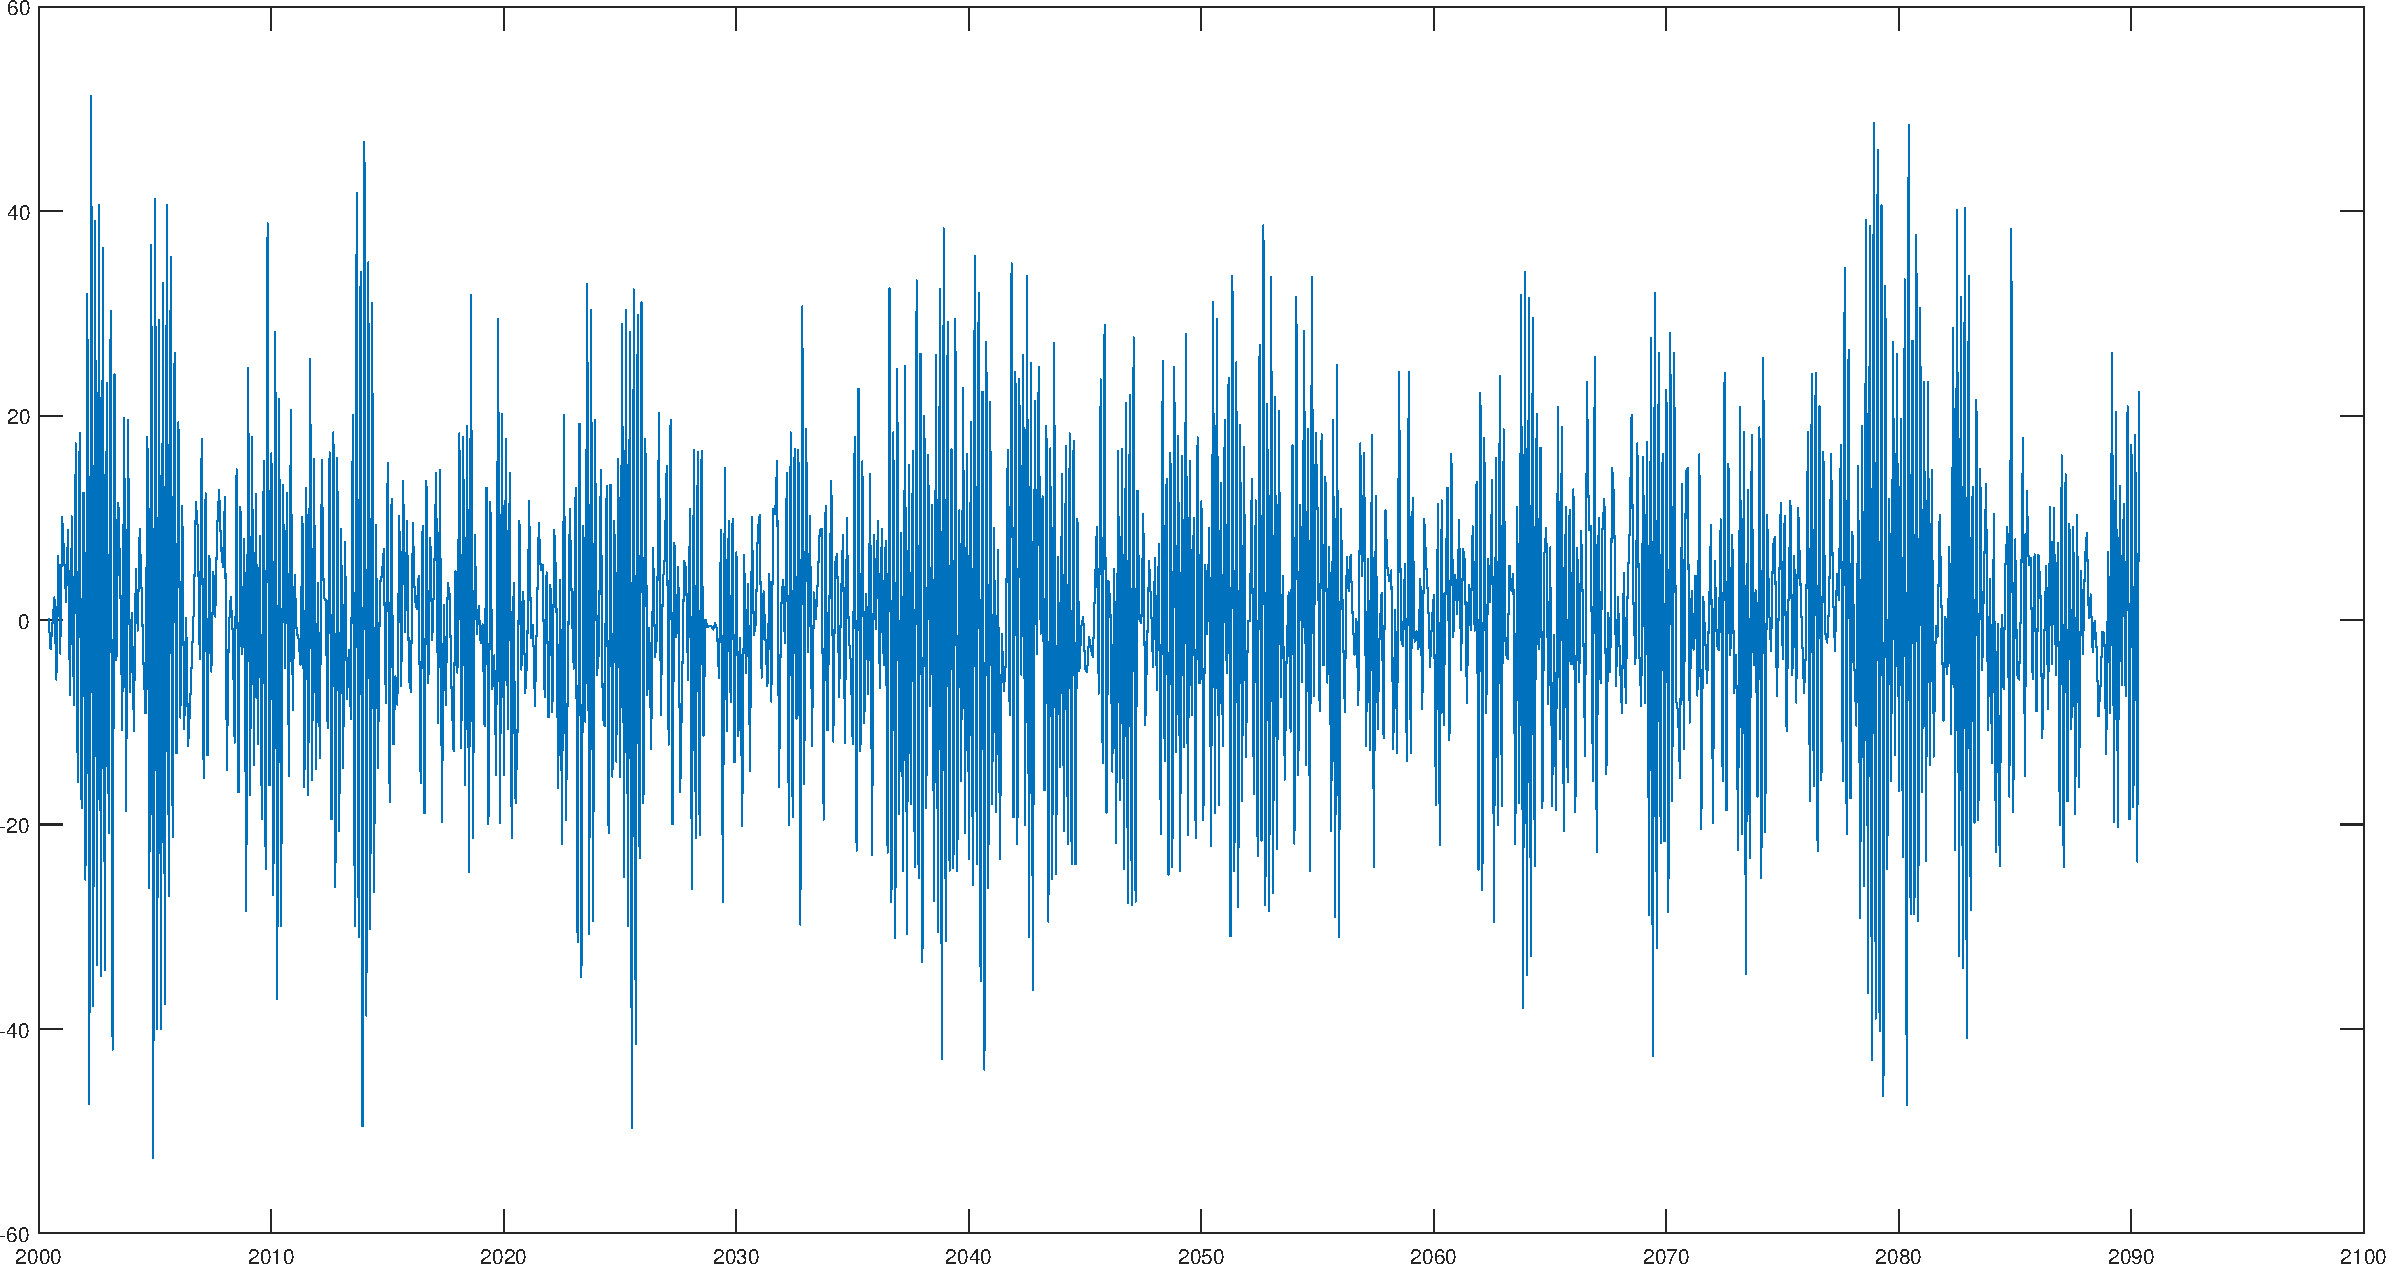
\includegraphics[width=1\linewidth]{inc/task1_noise}}
	\caption{Авто-регрессионный шум}
	\label{task1_noise}
\end{figure}

\newpage
Добавим его к сигналу  (рис. \ref{task1_signal_noise}):
\begin{figure}[!h]
	\center{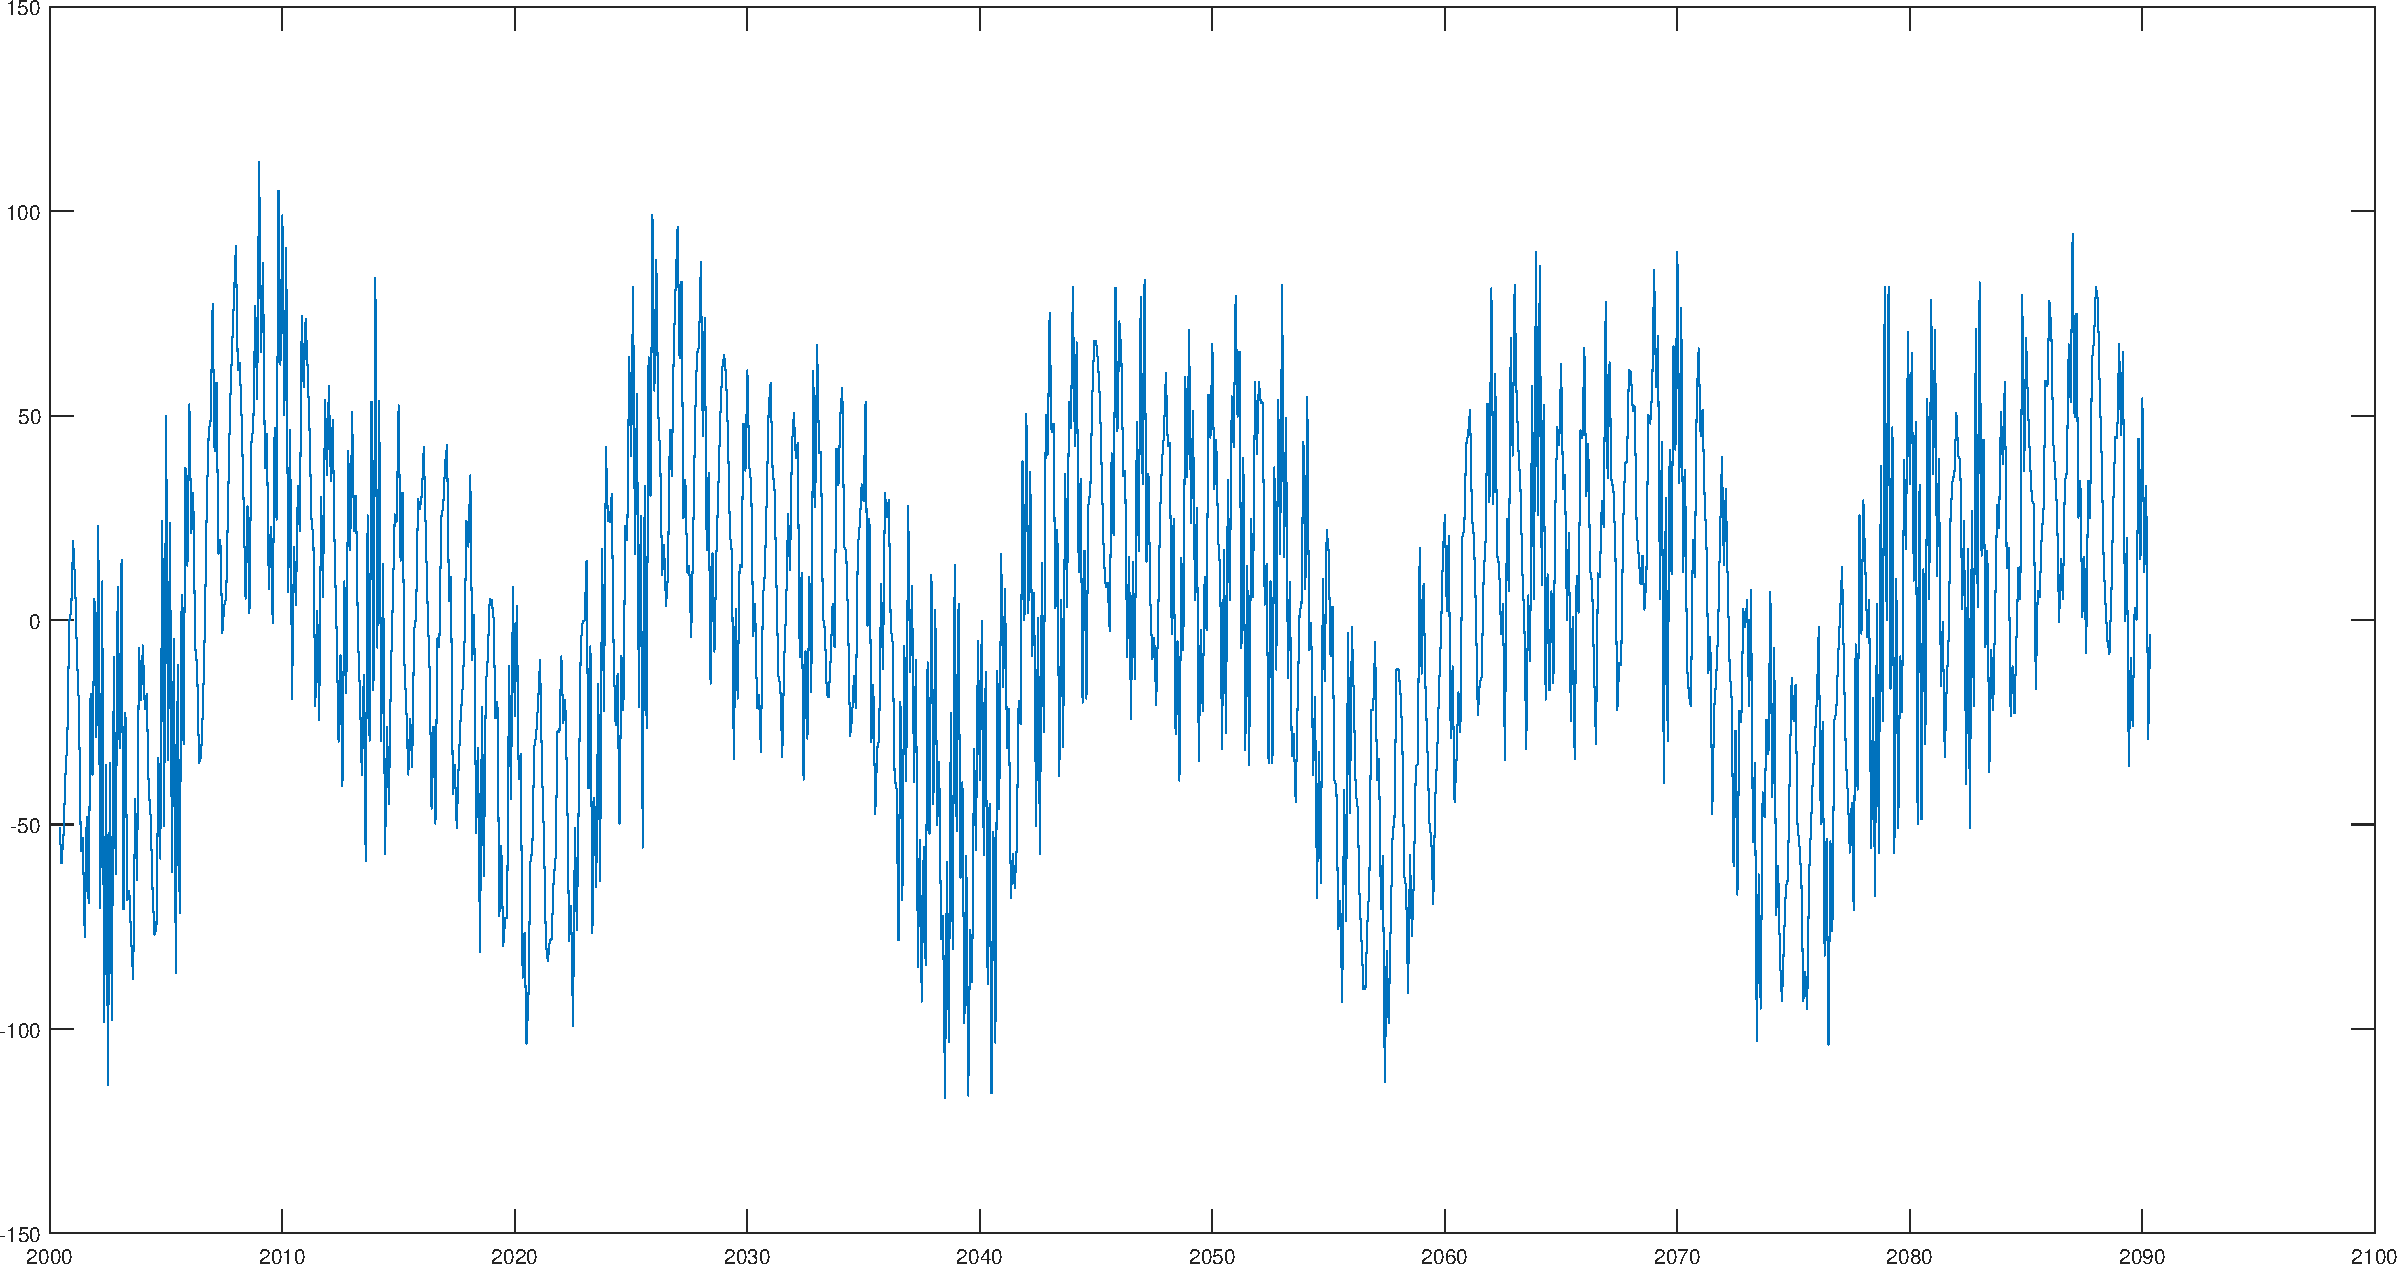
\includegraphics[width=1\linewidth]{inc/task1_signal_noise}}
	\caption{Сигнал с шумом}
	\label{task1_signal_noise}
\end{figure}

Вычислим смещенную оценку АКФ (рис. \ref{task1_acf_biased}):
\begin{figure}[!h]
	\center{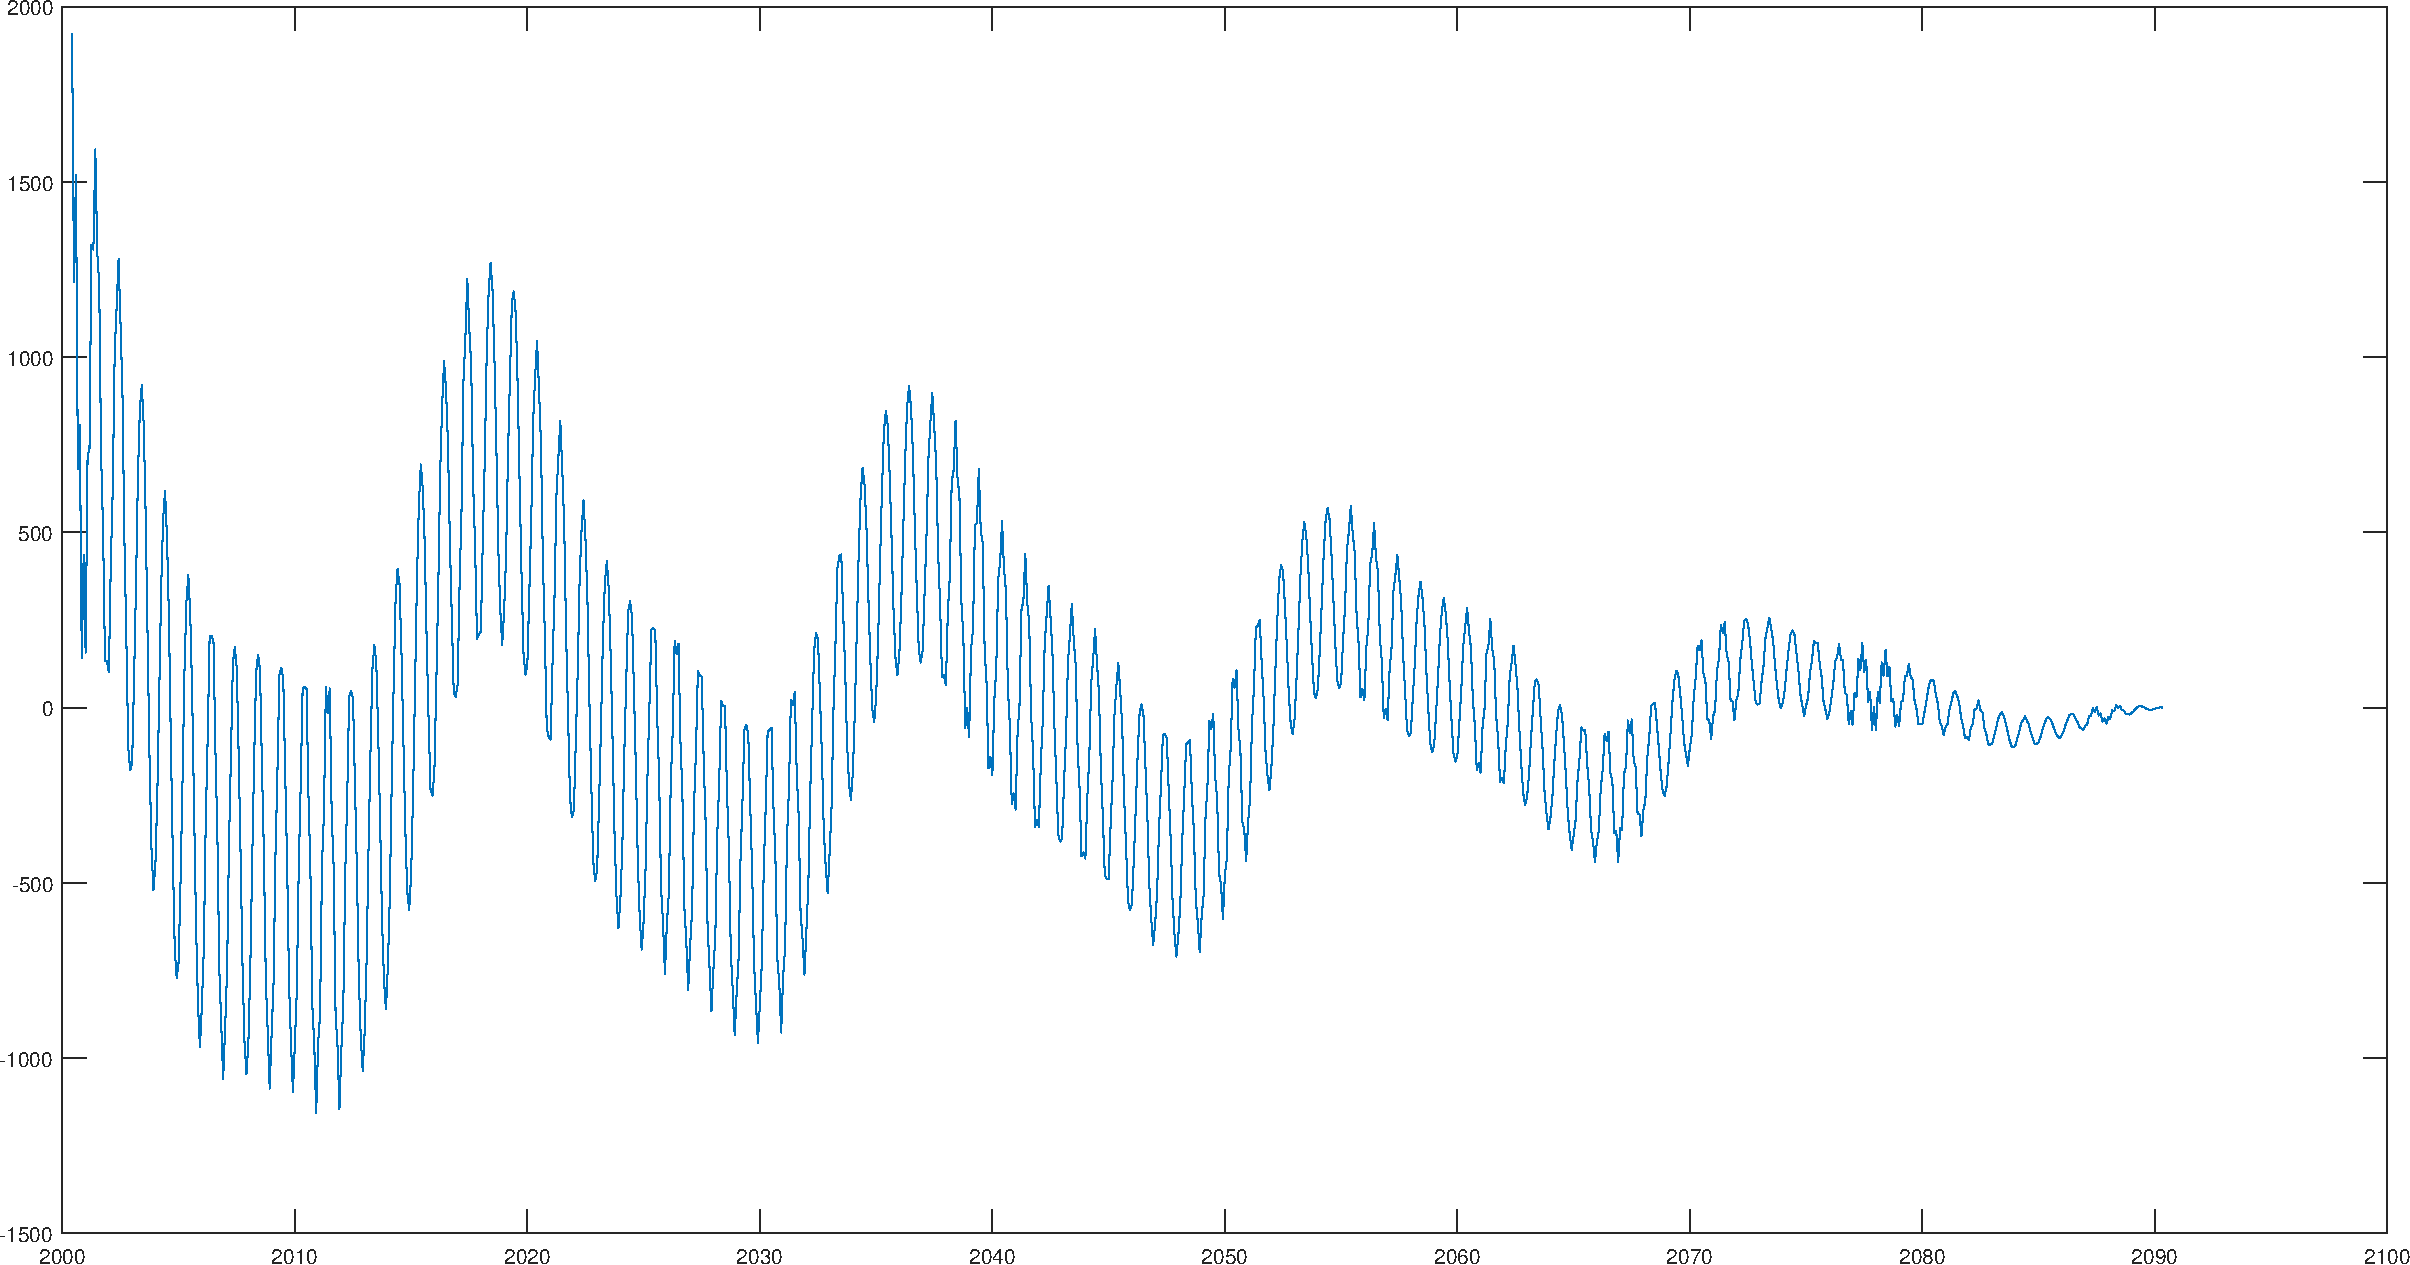
\includegraphics[width=1\linewidth]{inc/task1_acf_biased}}
	\caption{Cмещенная АКФ}
	\label{task1_acf_biased}
\end{figure}

\newpage
Вычислим несмещенную оценку АКФ (рис. \ref{task1_acf_unbiased}):
\begin{figure}[!h]
	\center{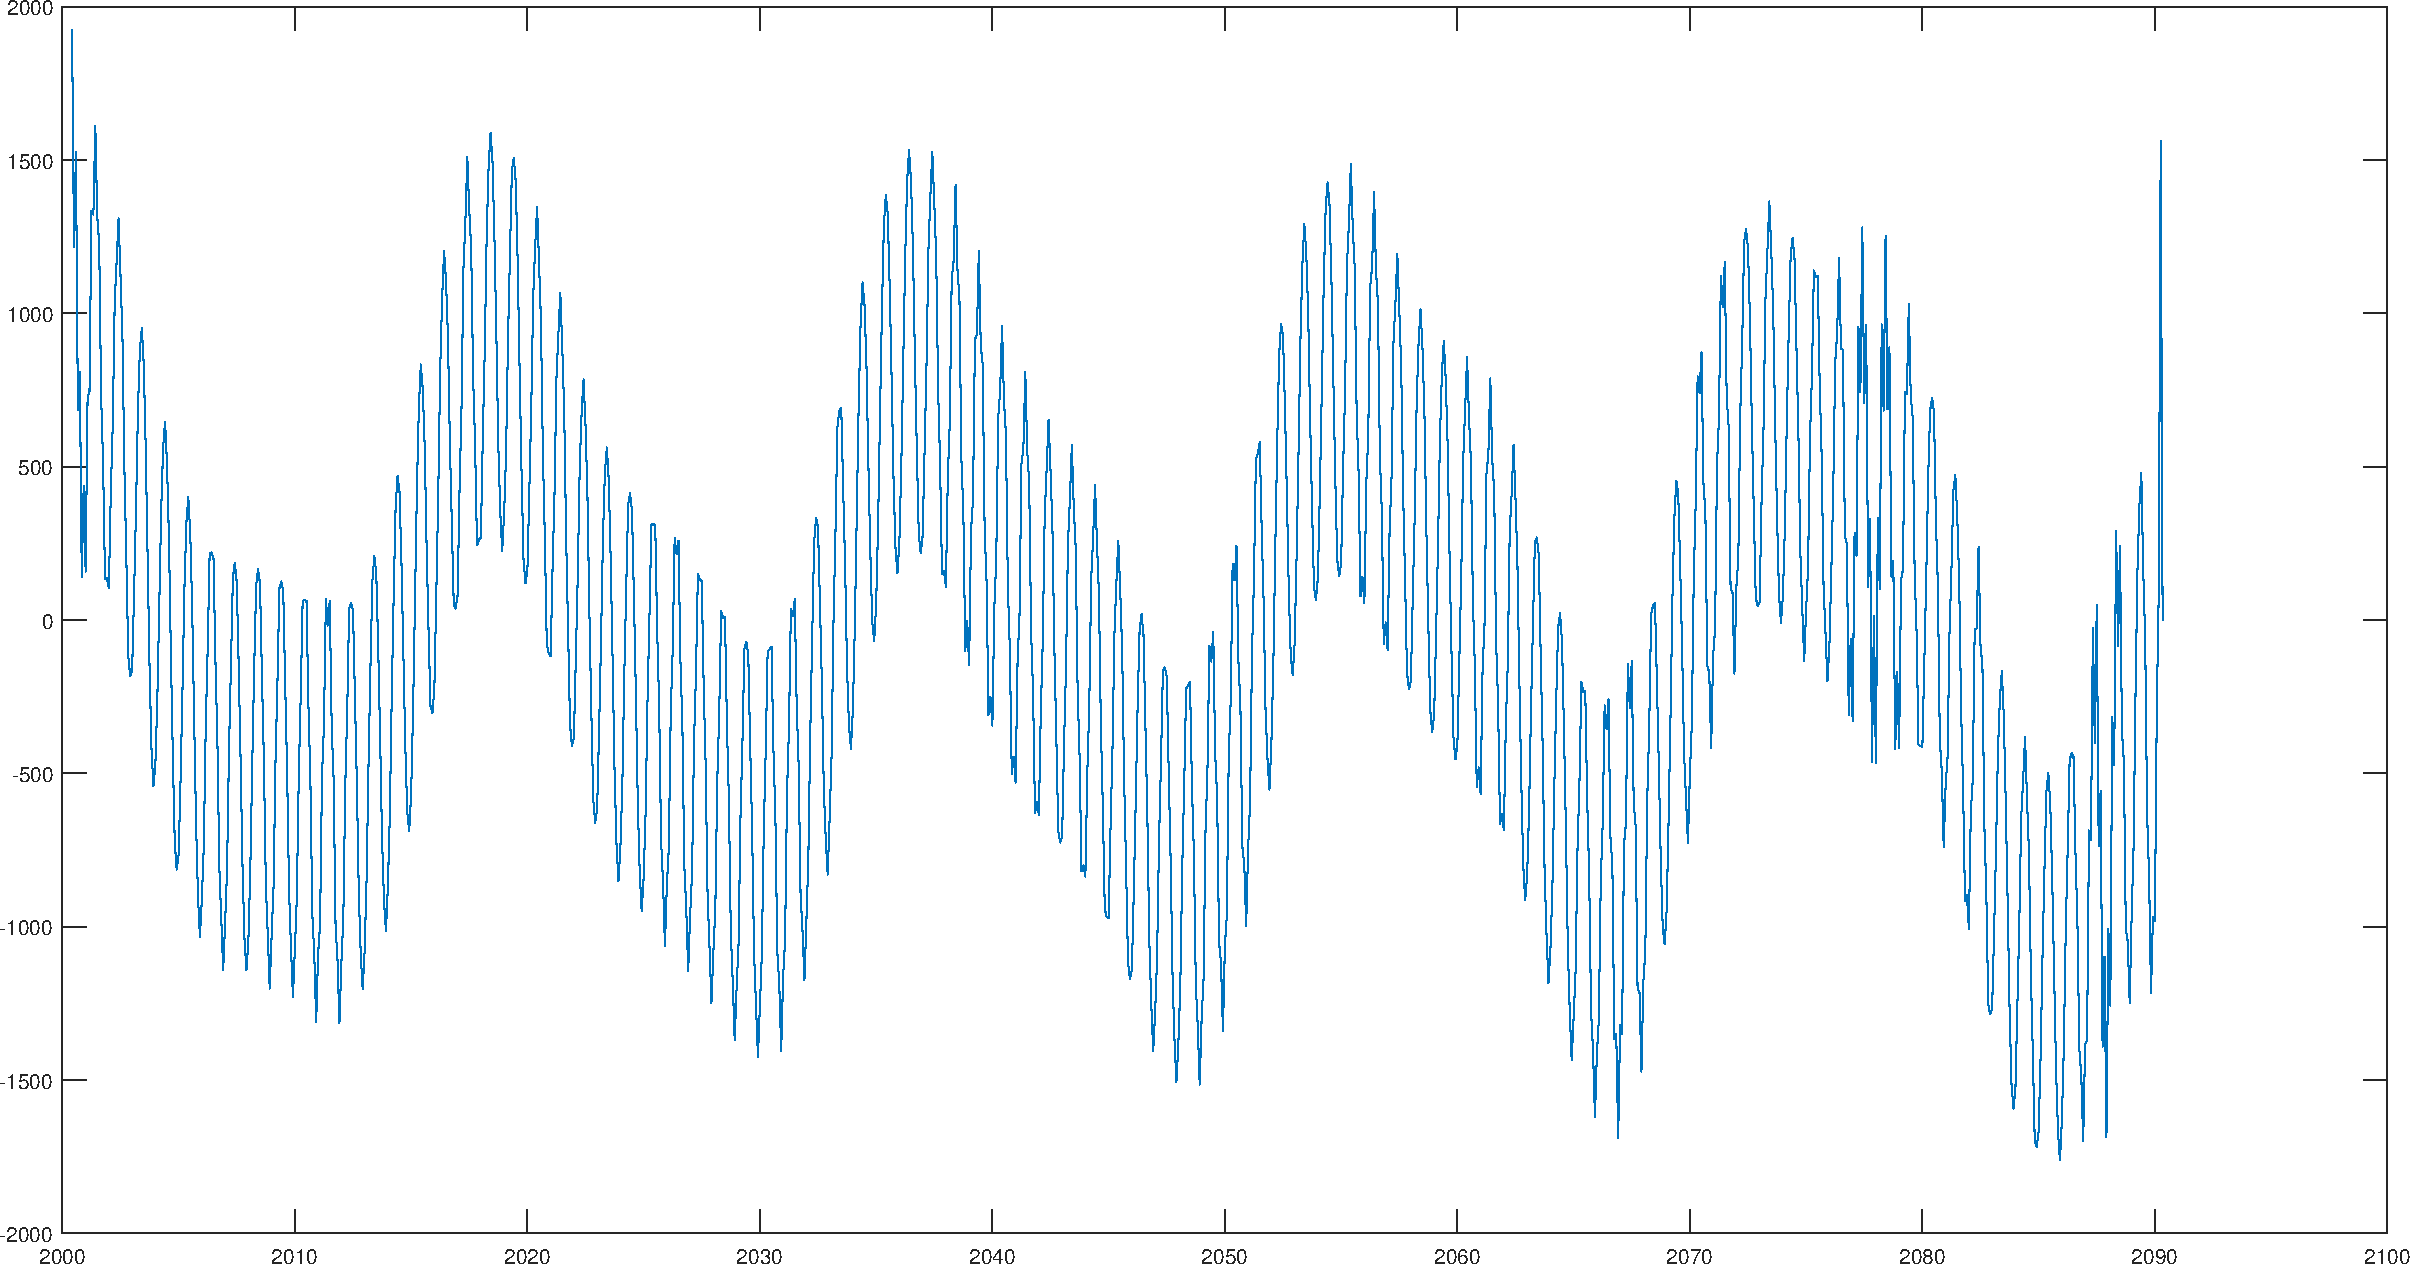
\includegraphics[width=1\linewidth]{inc/task1_acf_unbiased}}
	\caption{Несмещенная АКФ}
	\label{task1_acf_unbiased}
\end{figure}

Построим СПМ взятием фурье-преобразования смещенной и несмещенной АКФ (рис. \ref{task1_psd_biased}-\ref{task1_psd_unbiased}):
\begin{figure}[!h]
	\center{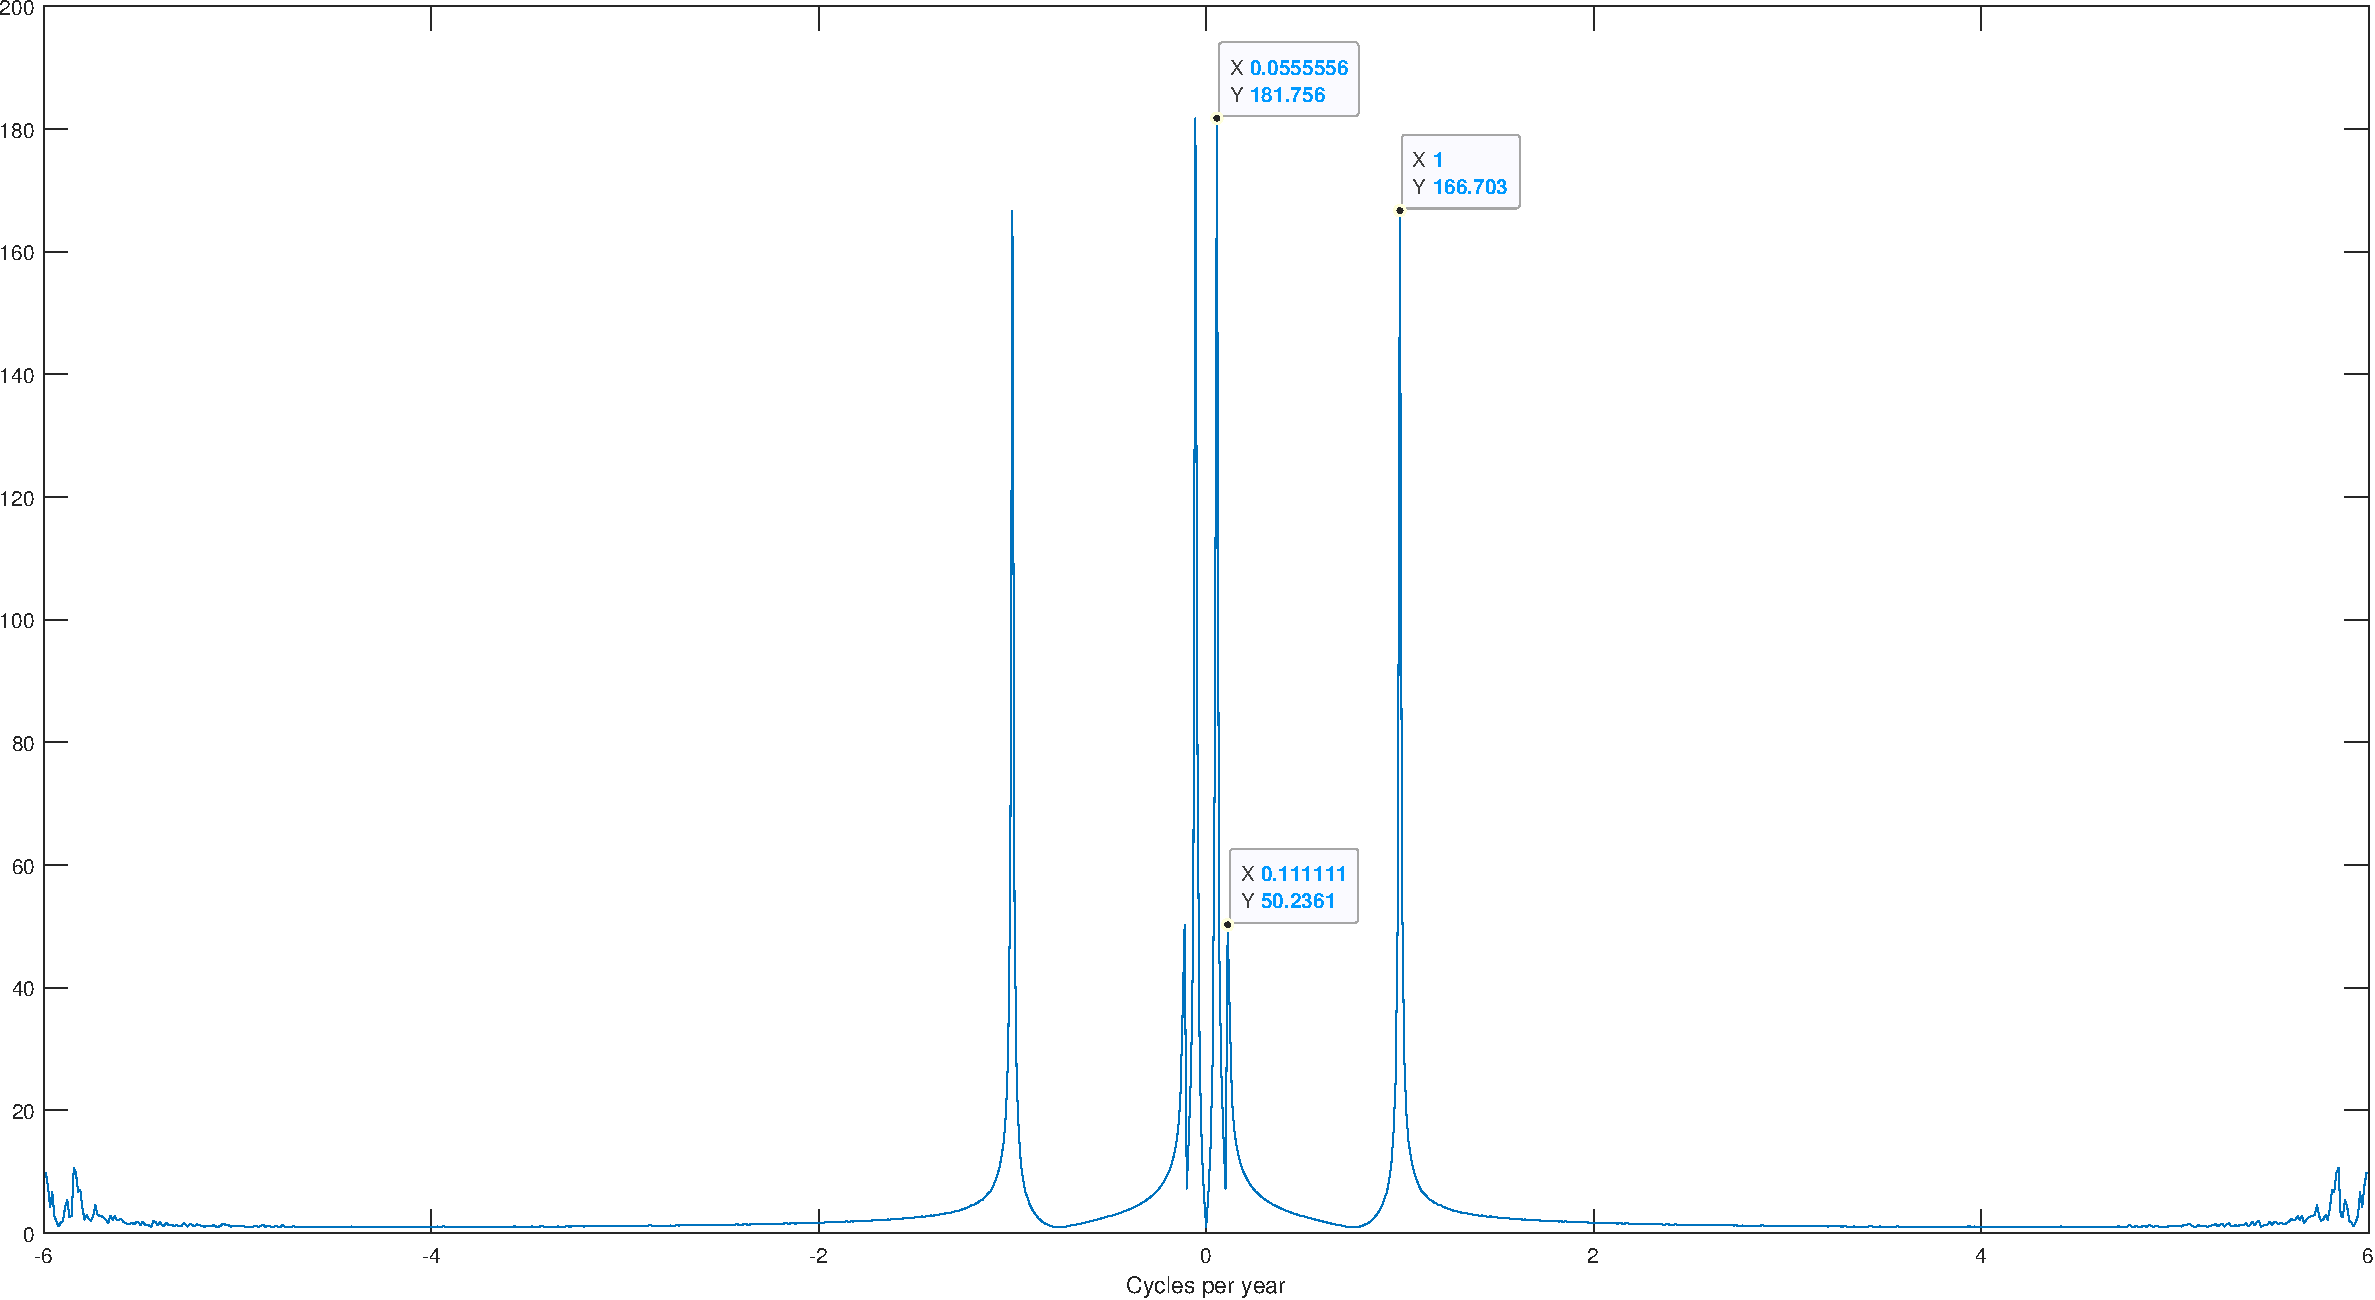
\includegraphics[width=1\linewidth]{inc/task1_psd_biased}}
	\caption{СПМ из смещенной АКФ}
	\label{task1_psd_biased}
\end{figure}

\newpage
\begin{figure}[!h]
\center{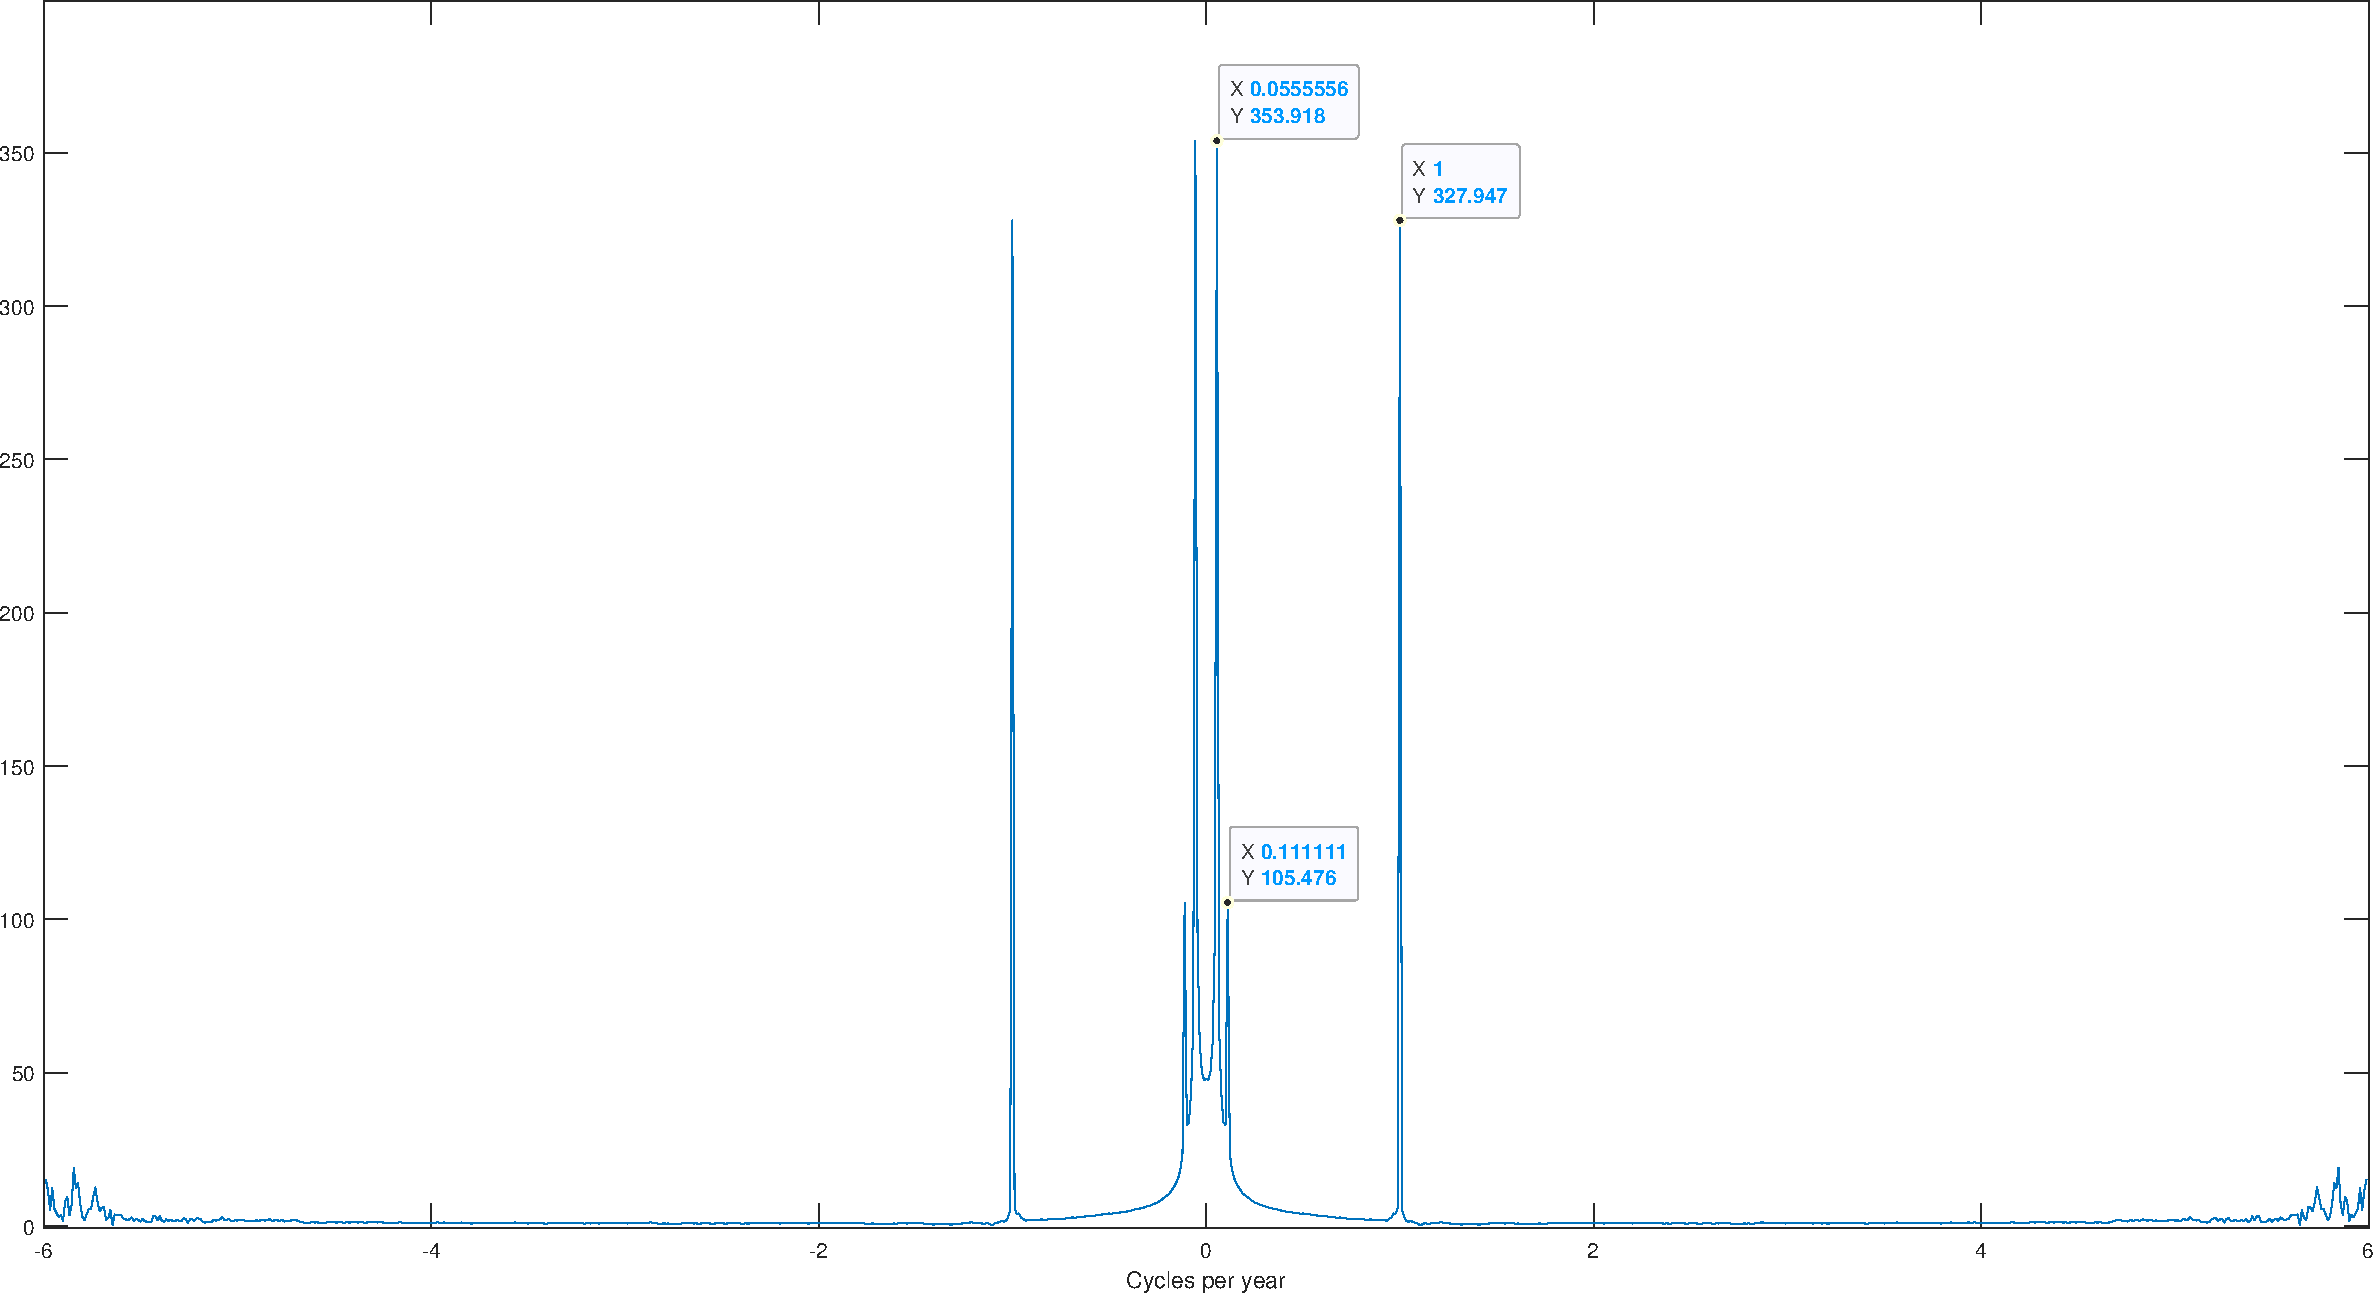
\includegraphics[width=1\linewidth]{inc/task1_psd_unbiased}}
\caption{СПМ из несмещенной АКФ}
\label{task1_psd_unbiased}
\end{figure}

\noindent По пиковым значениям можно проверить частоты изначальных гармоник: 

\noindent $1 \text{ цикл в год, } \frac{1}{1} = 1 \text{, что соответствует гармонике с периодом 1 год}$

\noindent $0.(1) \text{ цикл в год, } \frac{1}{0.111111} \approx 9\text{, что соответствует гармонике с периодом 8.86 год}$

\noindent $0.0(5) \text{ цикл в год, } \frac{1}{0.055556} \approx 18\text{, что соответствует гармонике с периодом 18.6 год}$

\noindent Также, по краям спектра видно отражение наличия цветного шума.

\newpage
\textbf{Часть 2}

Теперь попробуем спрогнозировать индекс явления El Nino Southern Oscillation - ENSO BEST. Считаем данные из файла (рис. \ref{task2_data}):
\begin{figure}[!h]
	\center{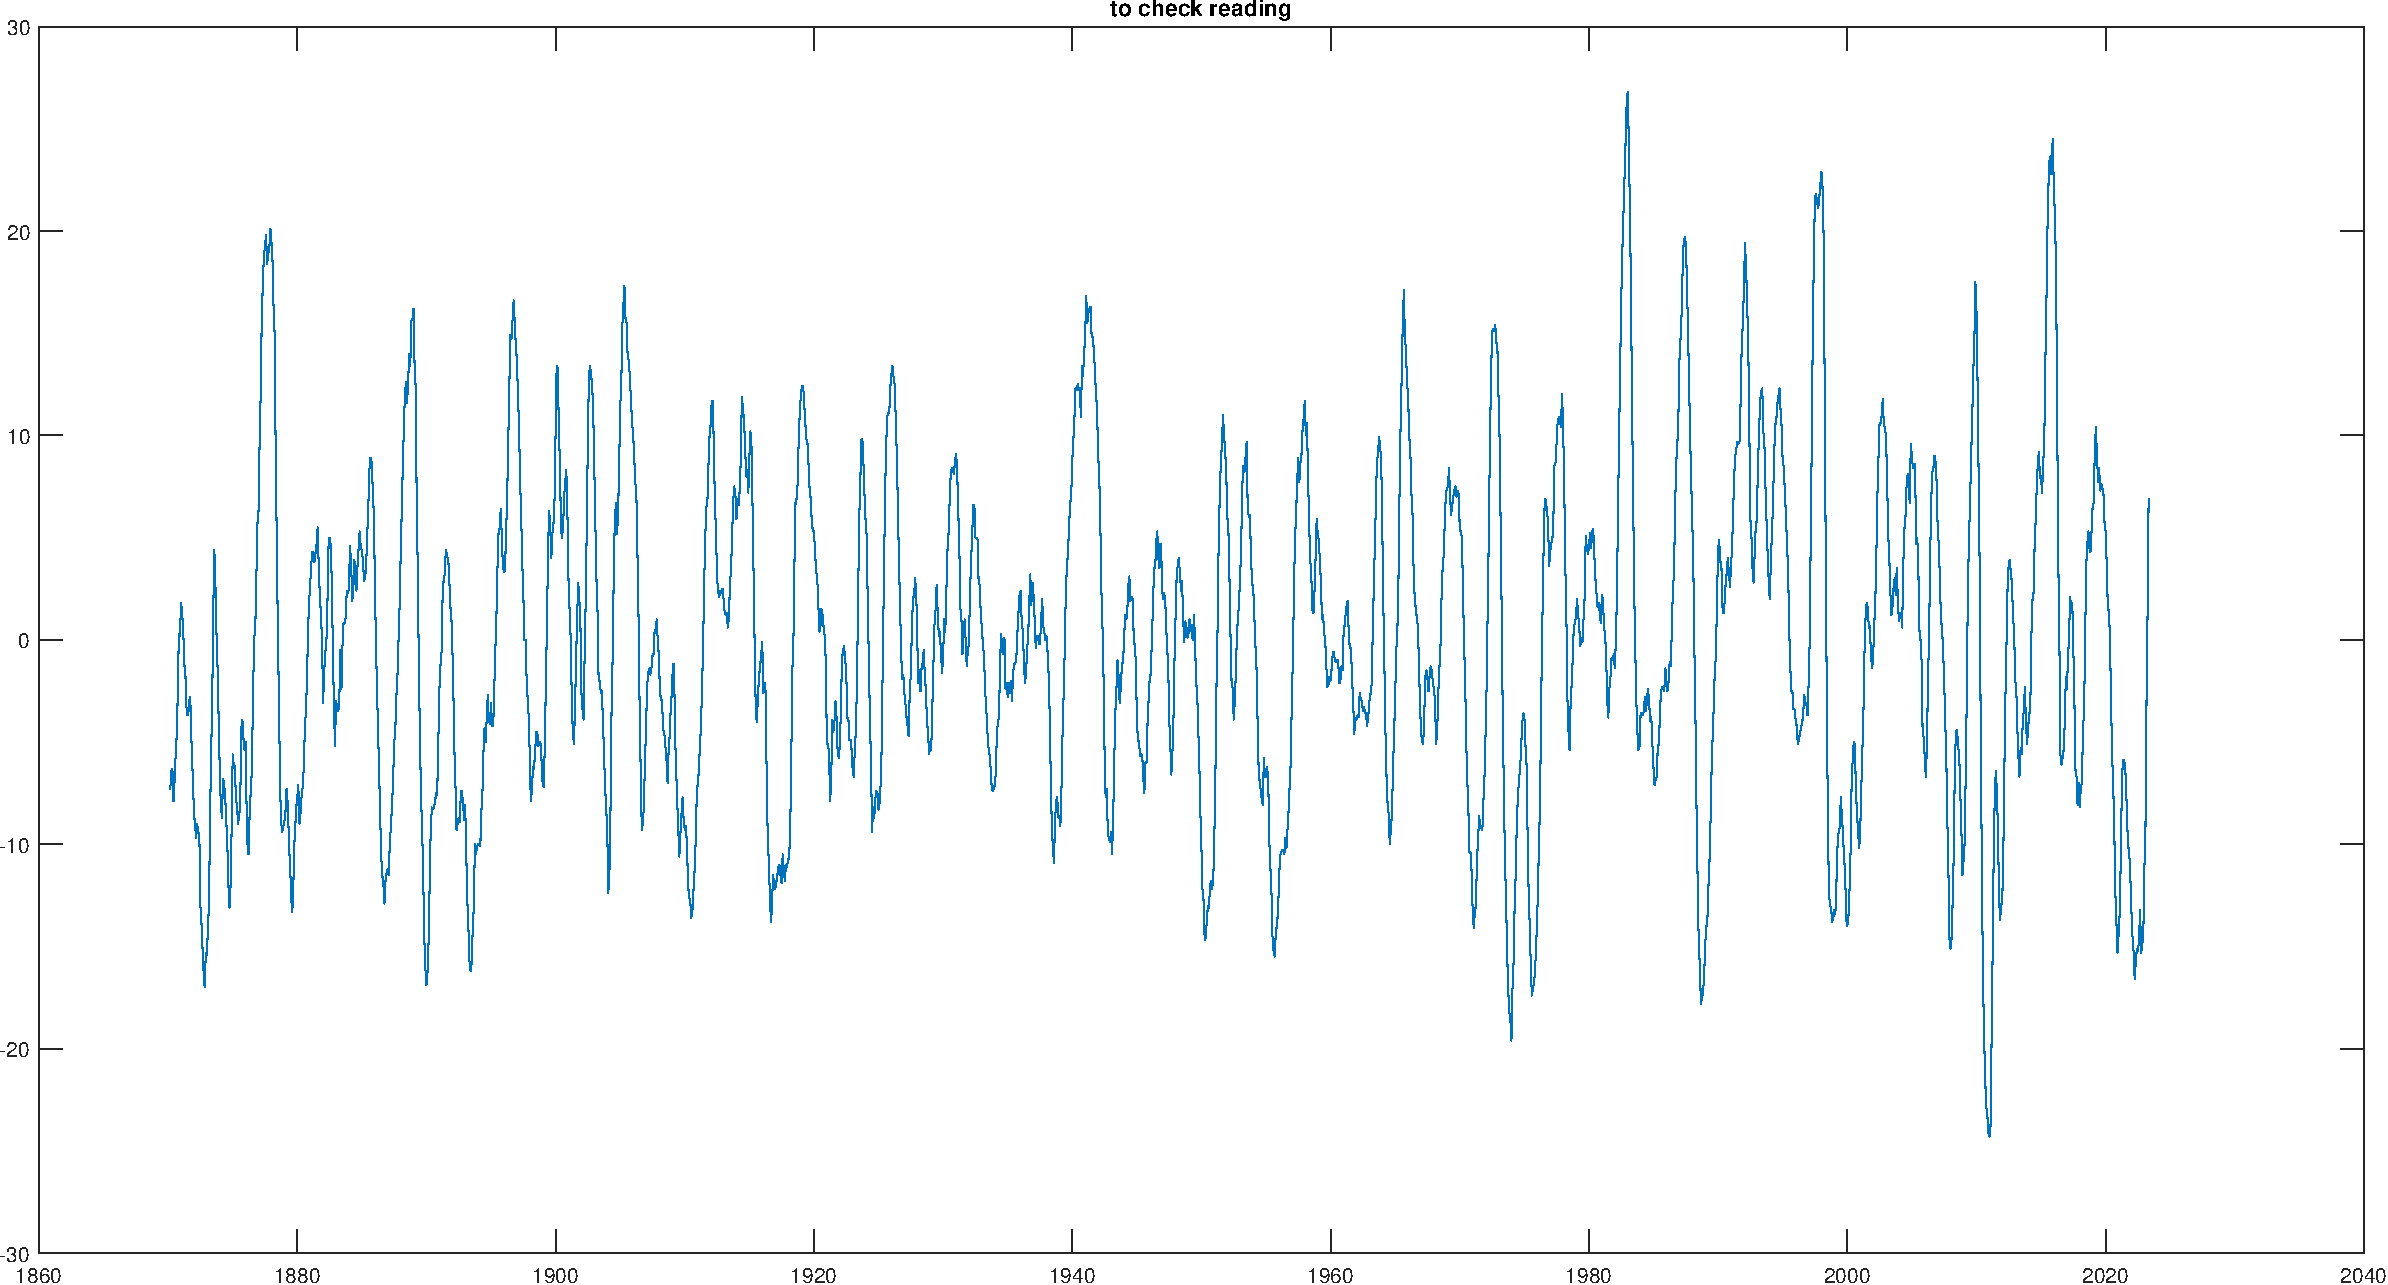
\includegraphics[width=1\linewidth]{inc/task2_data}}
	\caption{Данные из файла ENSO\_BEST\_index.dat}
	\label{task2_data}
\end{figure}

Вычислим смещенную и несмещенную оценку АКФ (рис. \ref{task2_acf_biased}-\ref{task2_acf_unbiased}):
\begin{figure}[!h]
	\center{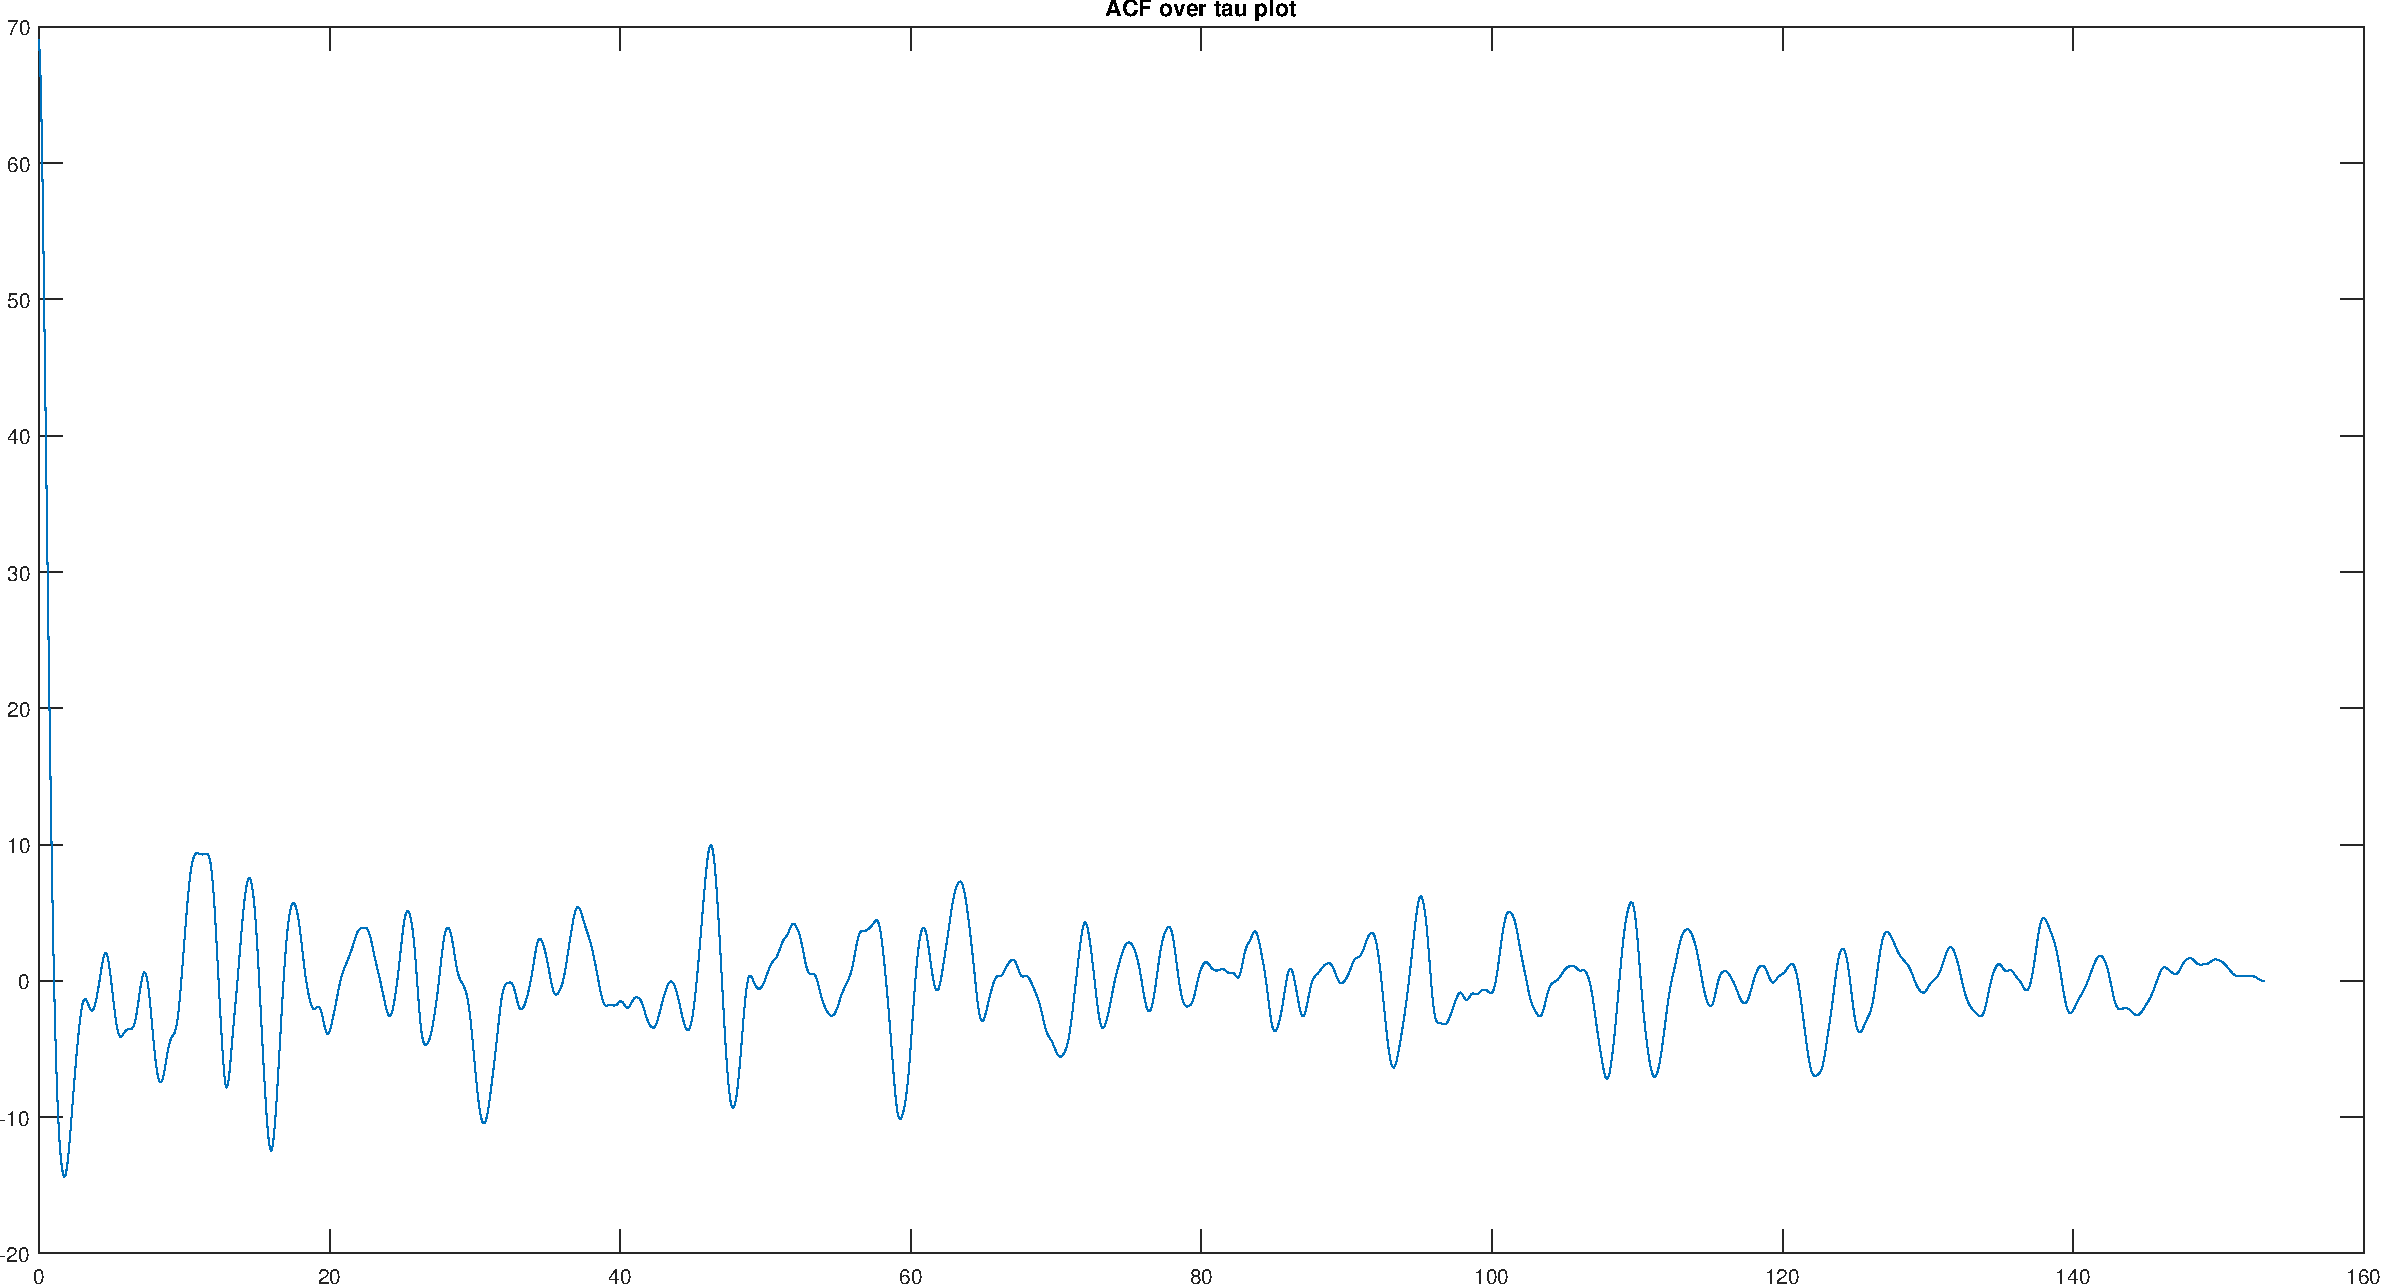
\includegraphics[width=1\linewidth]{inc/task2_acf_biased}}
	\caption{Cмещенная АКФ}
	\label{task2_acf_biased}
\end{figure}

\newpage
\begin{figure}[!h]
	\center{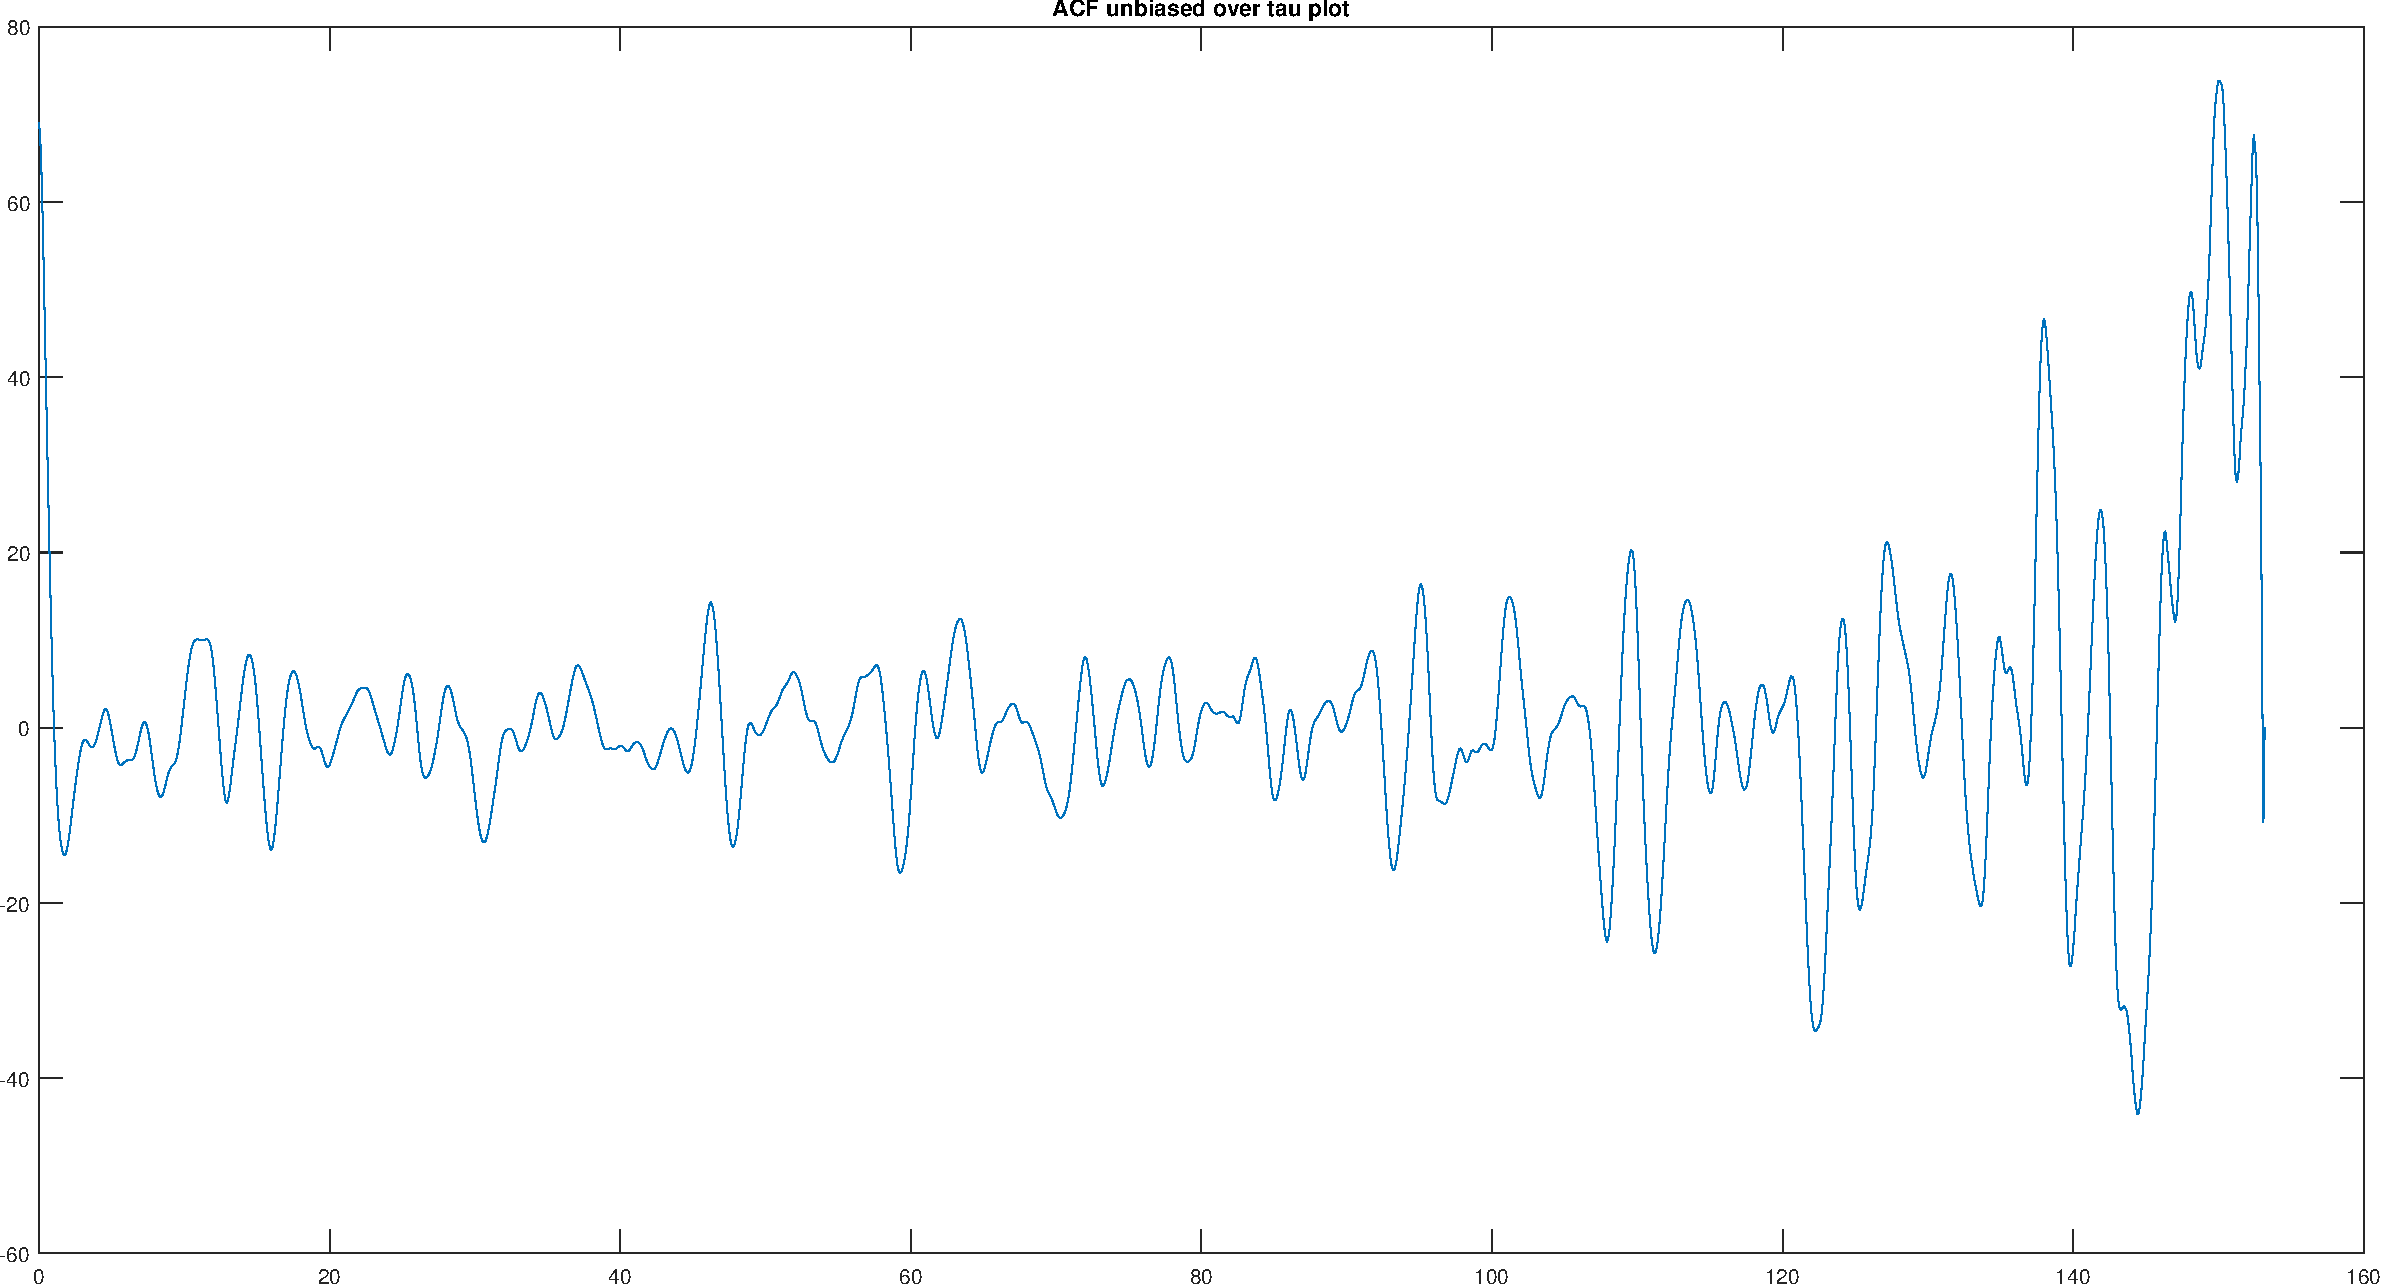
\includegraphics[width=1\linewidth]{inc/task2_acf_unbiased}}
	\caption{Несмещенная АКФ}
	\label{task2_acf_unbiased}
\end{figure}

Построим спектральную плотность для периодов (рис. \ref{task2_psd_periods}):
\begin{figure}[!h]
	\center{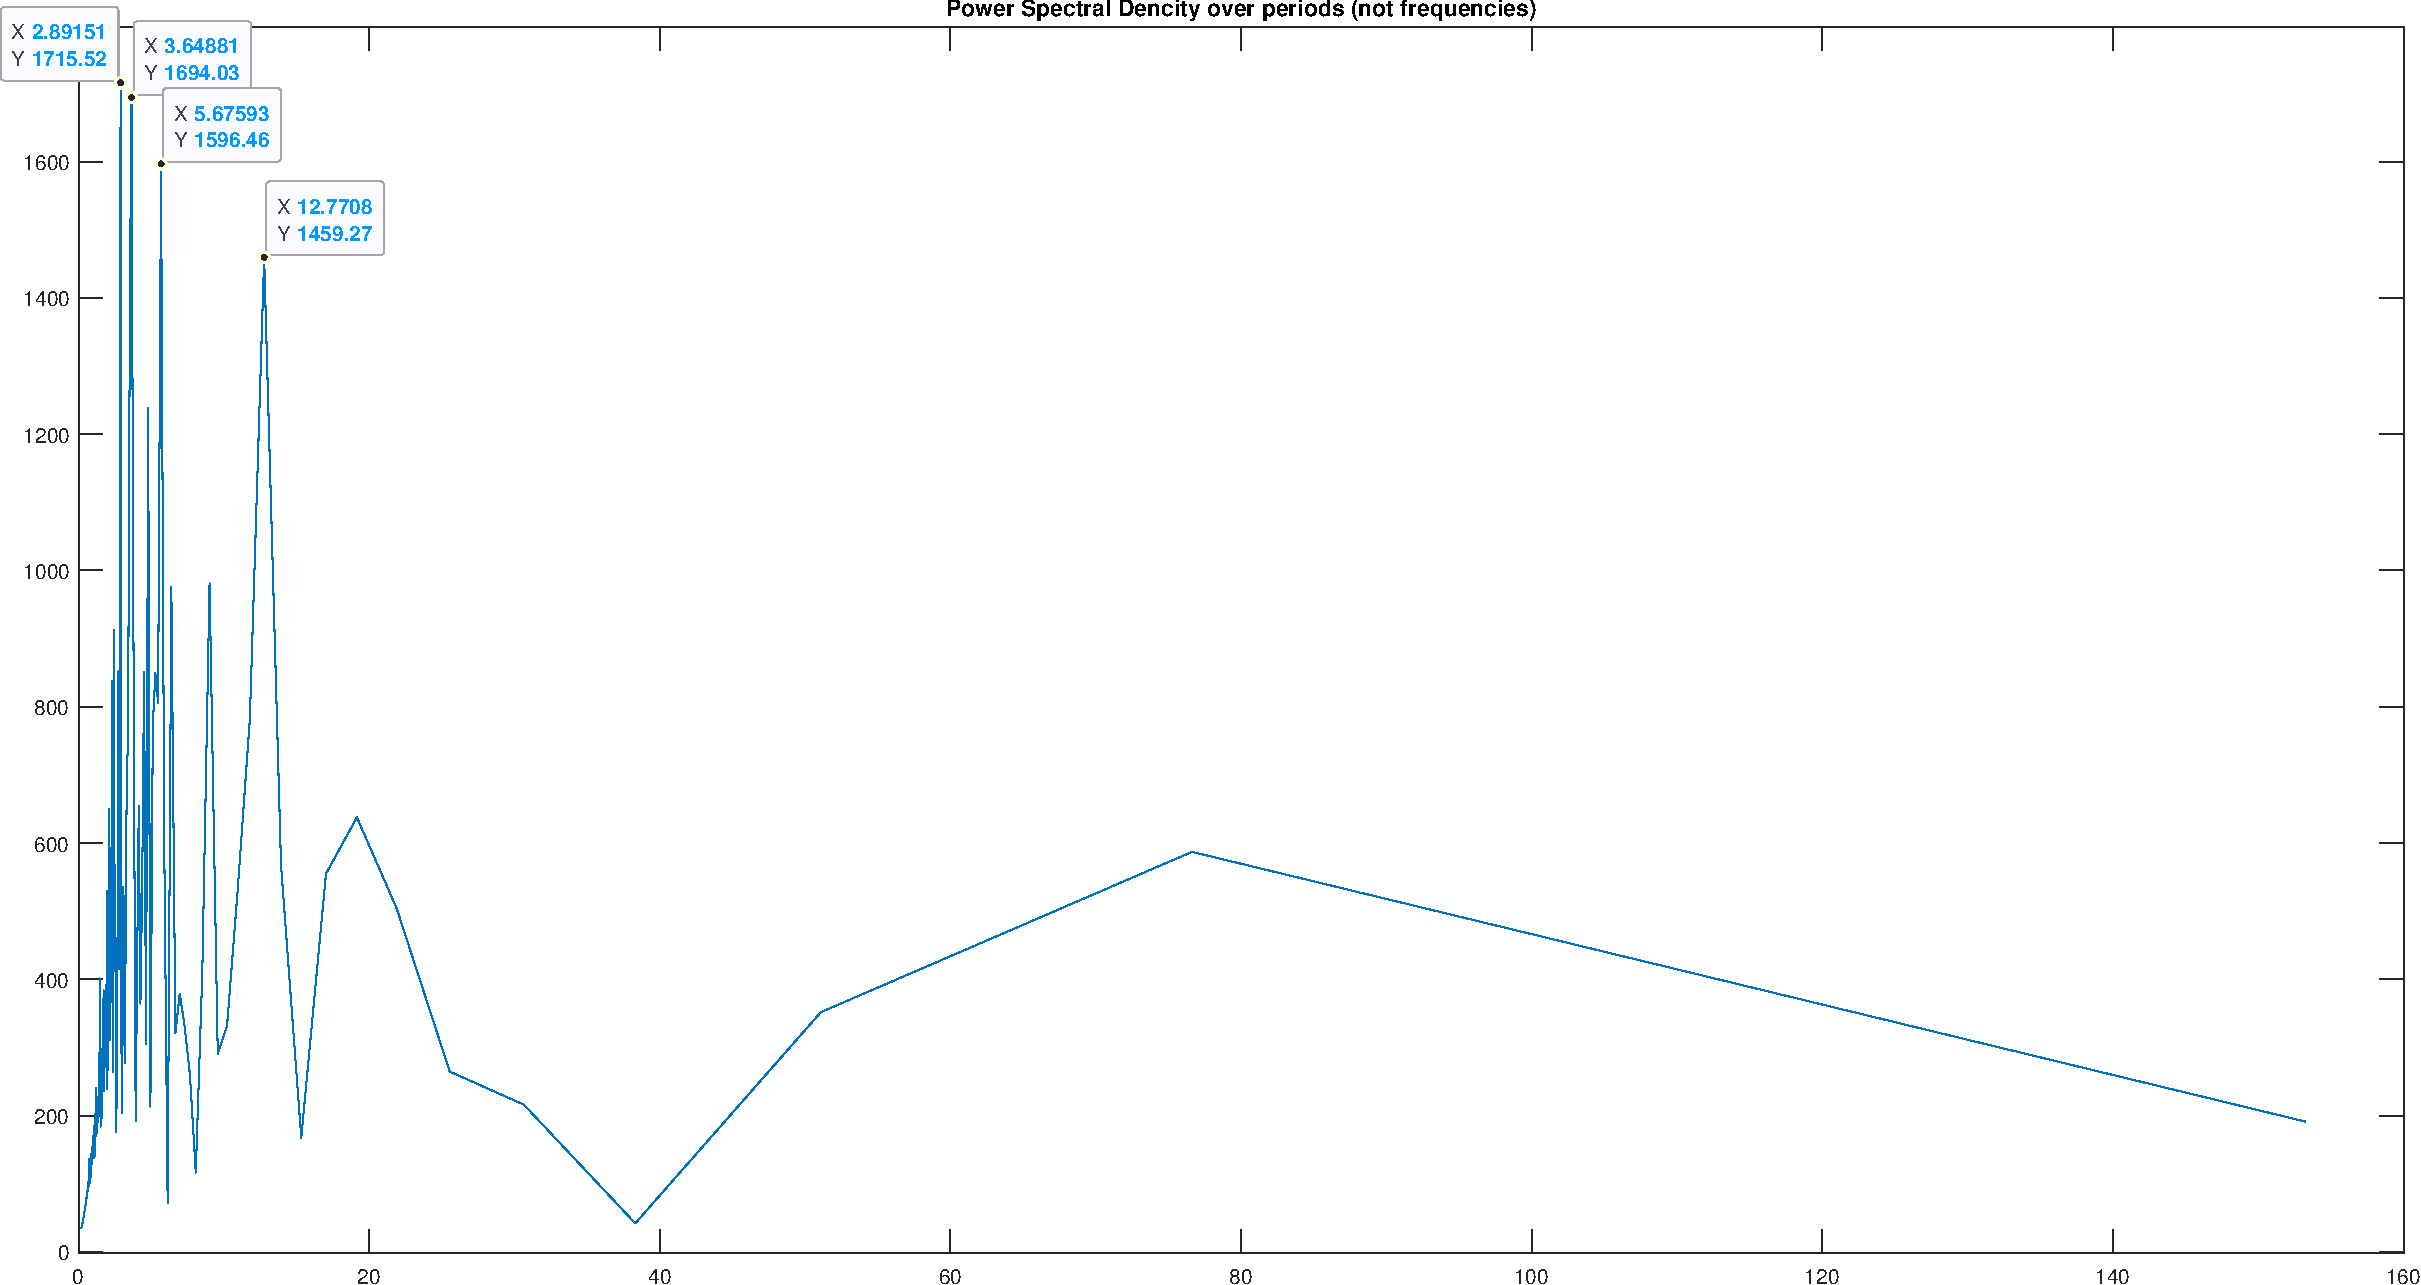
\includegraphics[width=1\linewidth]{inc/task2_psd_periods}}
	\caption{СПМ для периодов}
	\label{task2_psd_periods}
\end{figure}

Выделим периоды: 2.89, 3.65, 5.68 и 12.77 для подбора гармоник в будущем.

\newpage
Подберем полиномиальную модель (возьмем порядок 2) и определим тренд (рис. \ref{task2_predict_poly}):
\begin{figure}[!h]
	\center{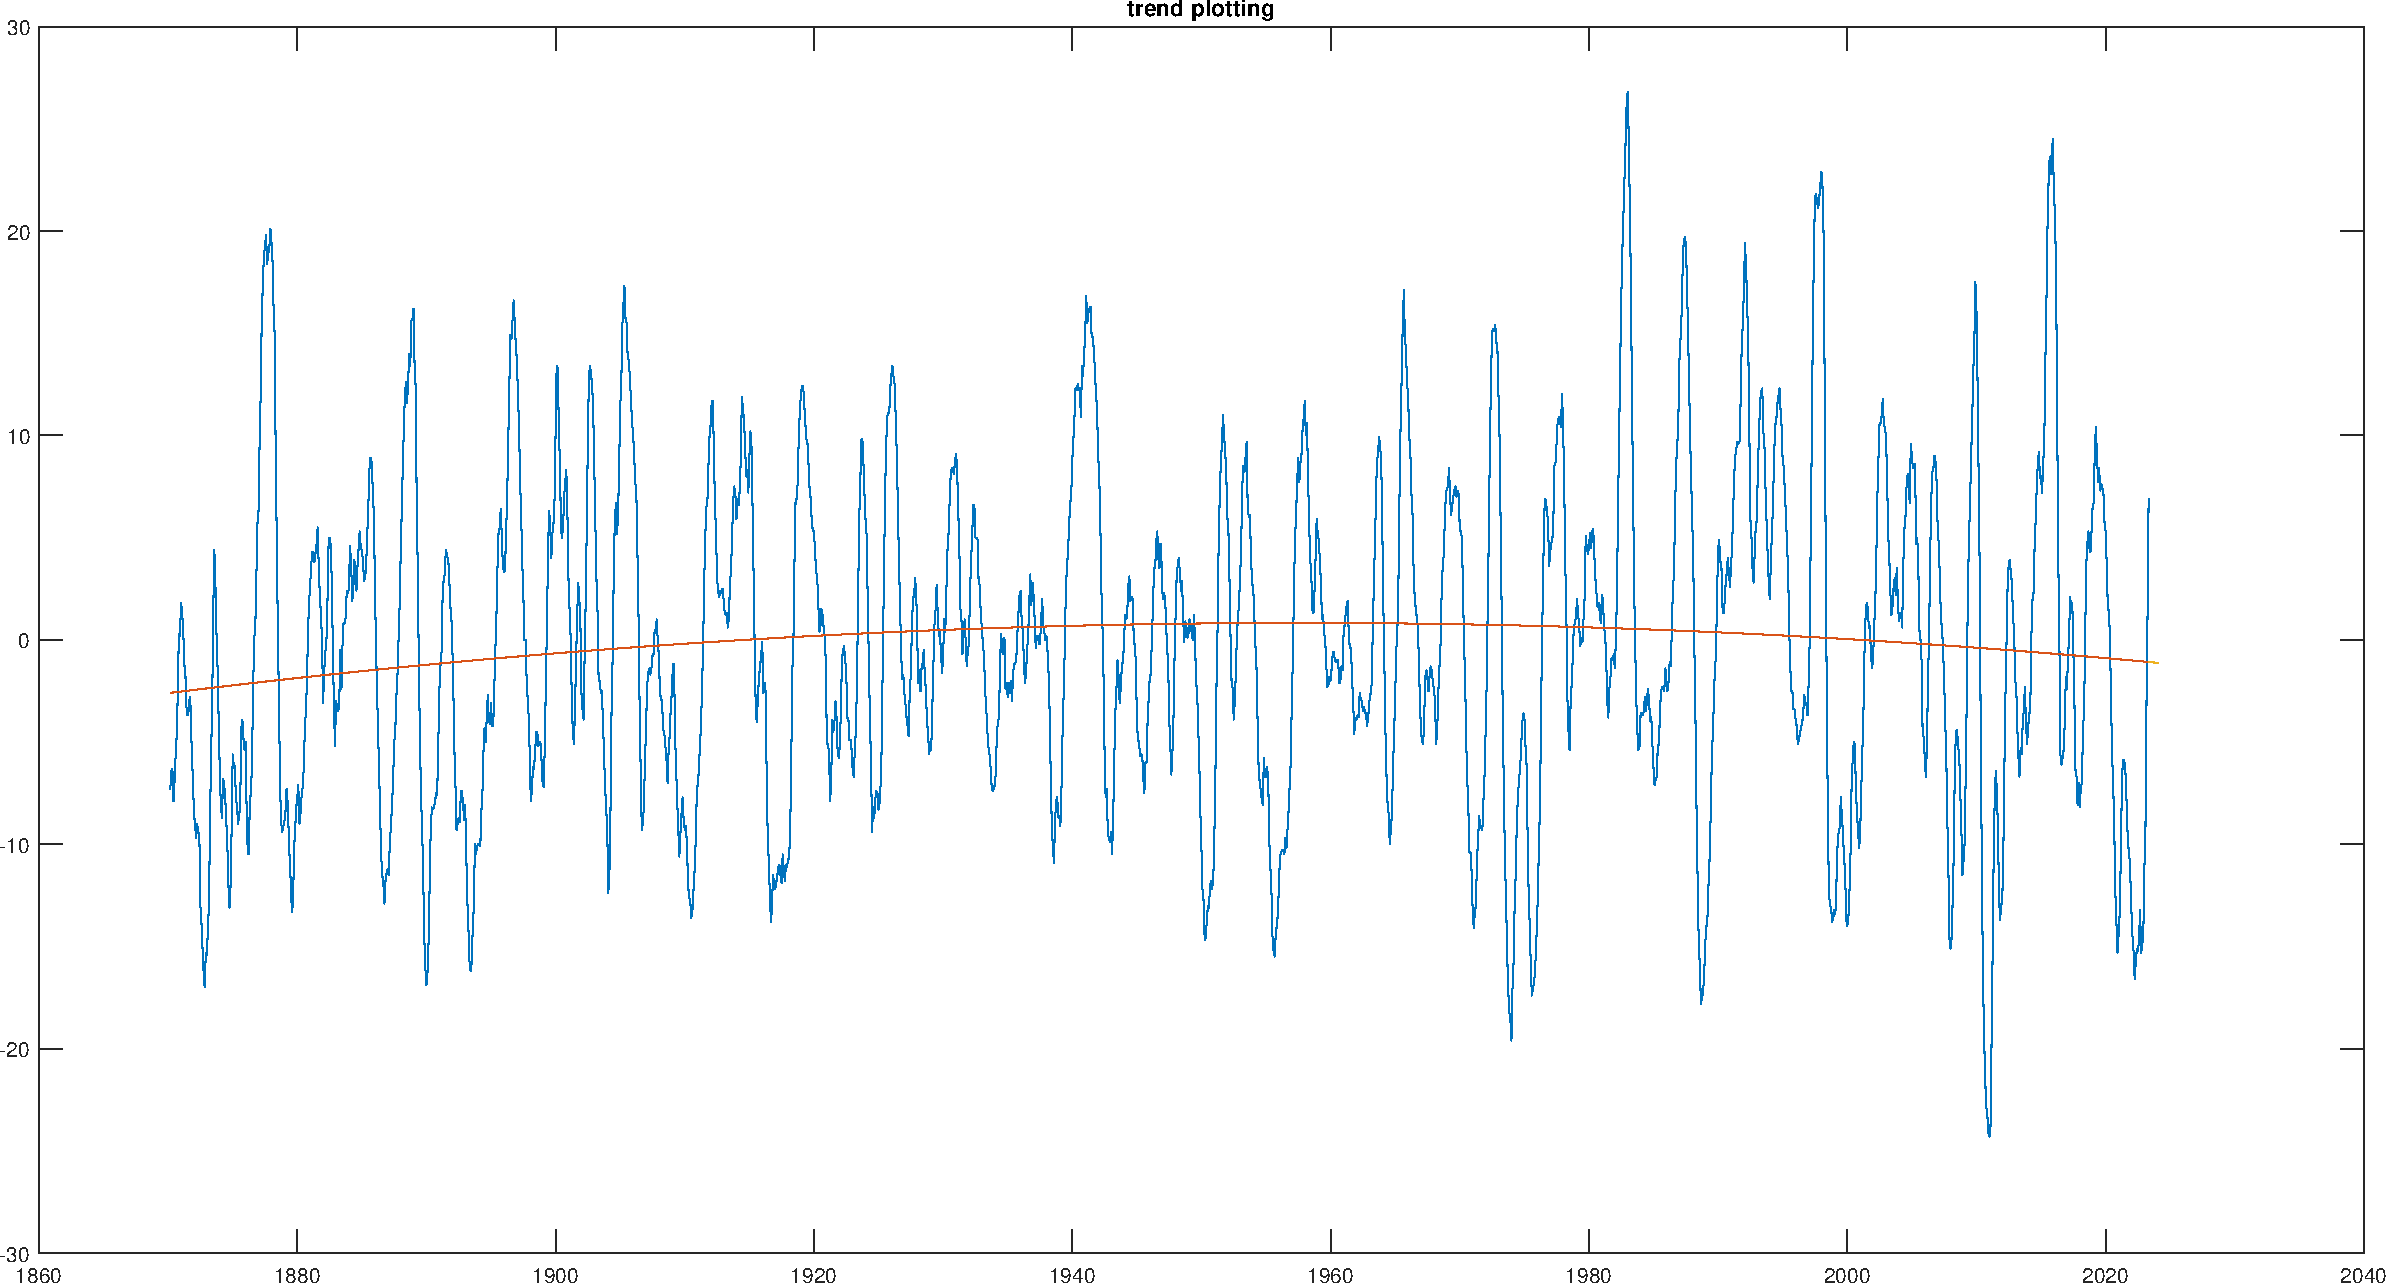
\includegraphics[width=1\linewidth]{inc/task2_predict_poly}}
	\caption{Тренд}
	\label{task2_predict_poly}
\end{figure}

Подберем гармоники задав периоды указанные выше (рис. \ref{task2_predict_harm}-\ref{task2_del_harm}):
\begin{figure}[!h]
	\center{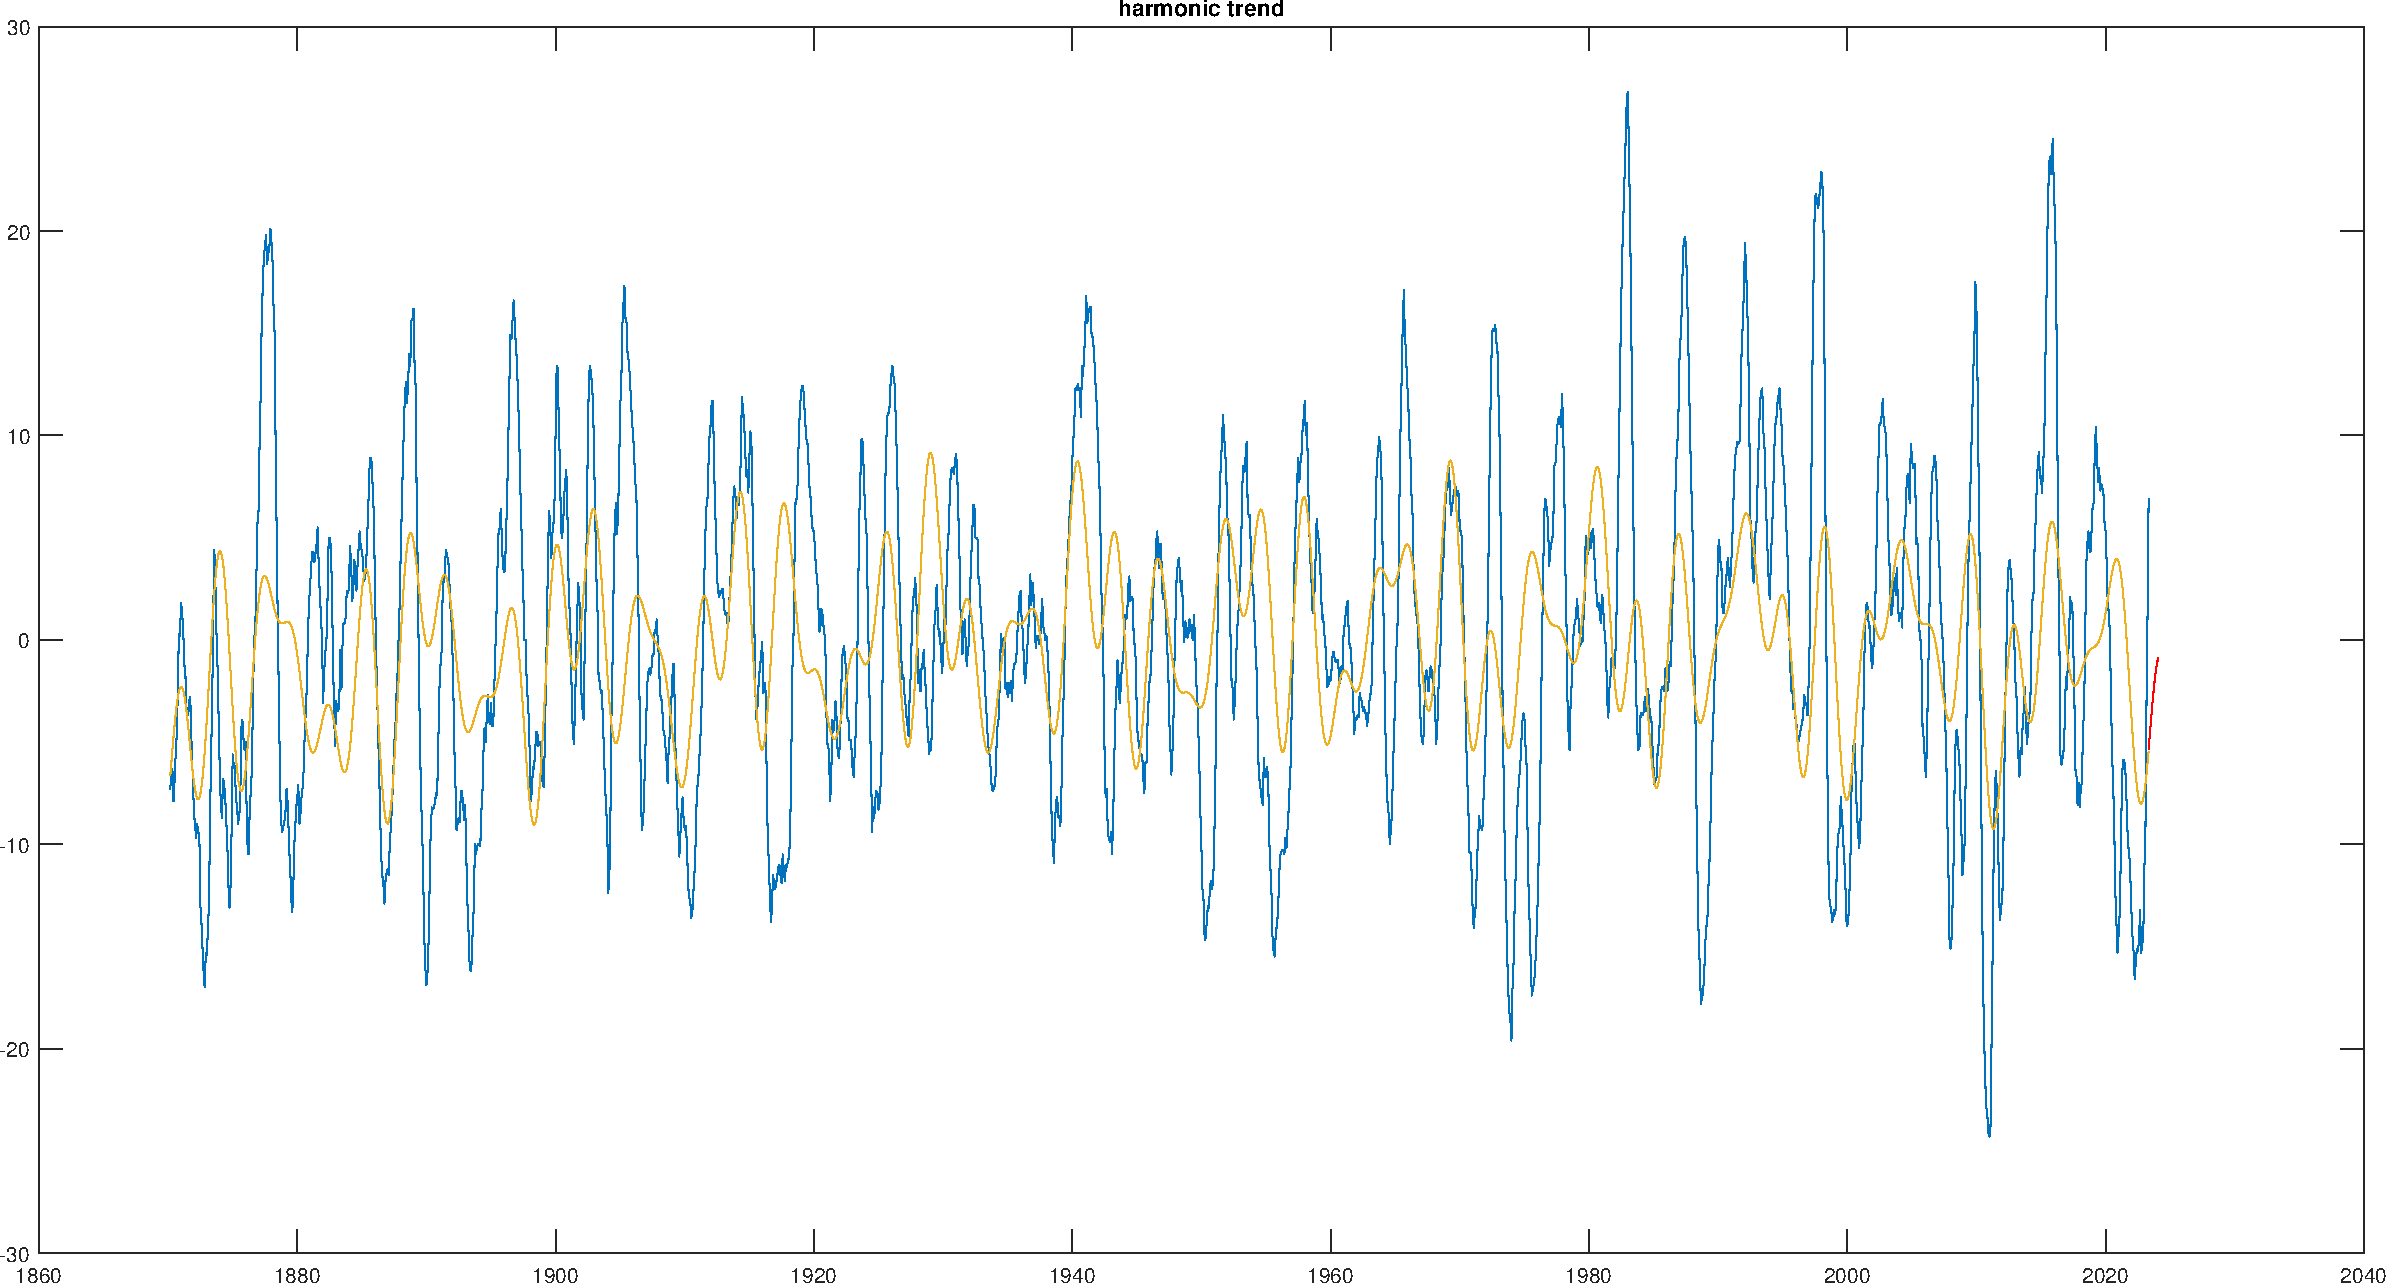
\includegraphics[width=1\linewidth]{inc/task2_predict_harm}}
	\caption{Тренд гармоник}
	\label{task2_predict_harm}
\end{figure}

\newpage
\begin{figure}[!h]
	\center{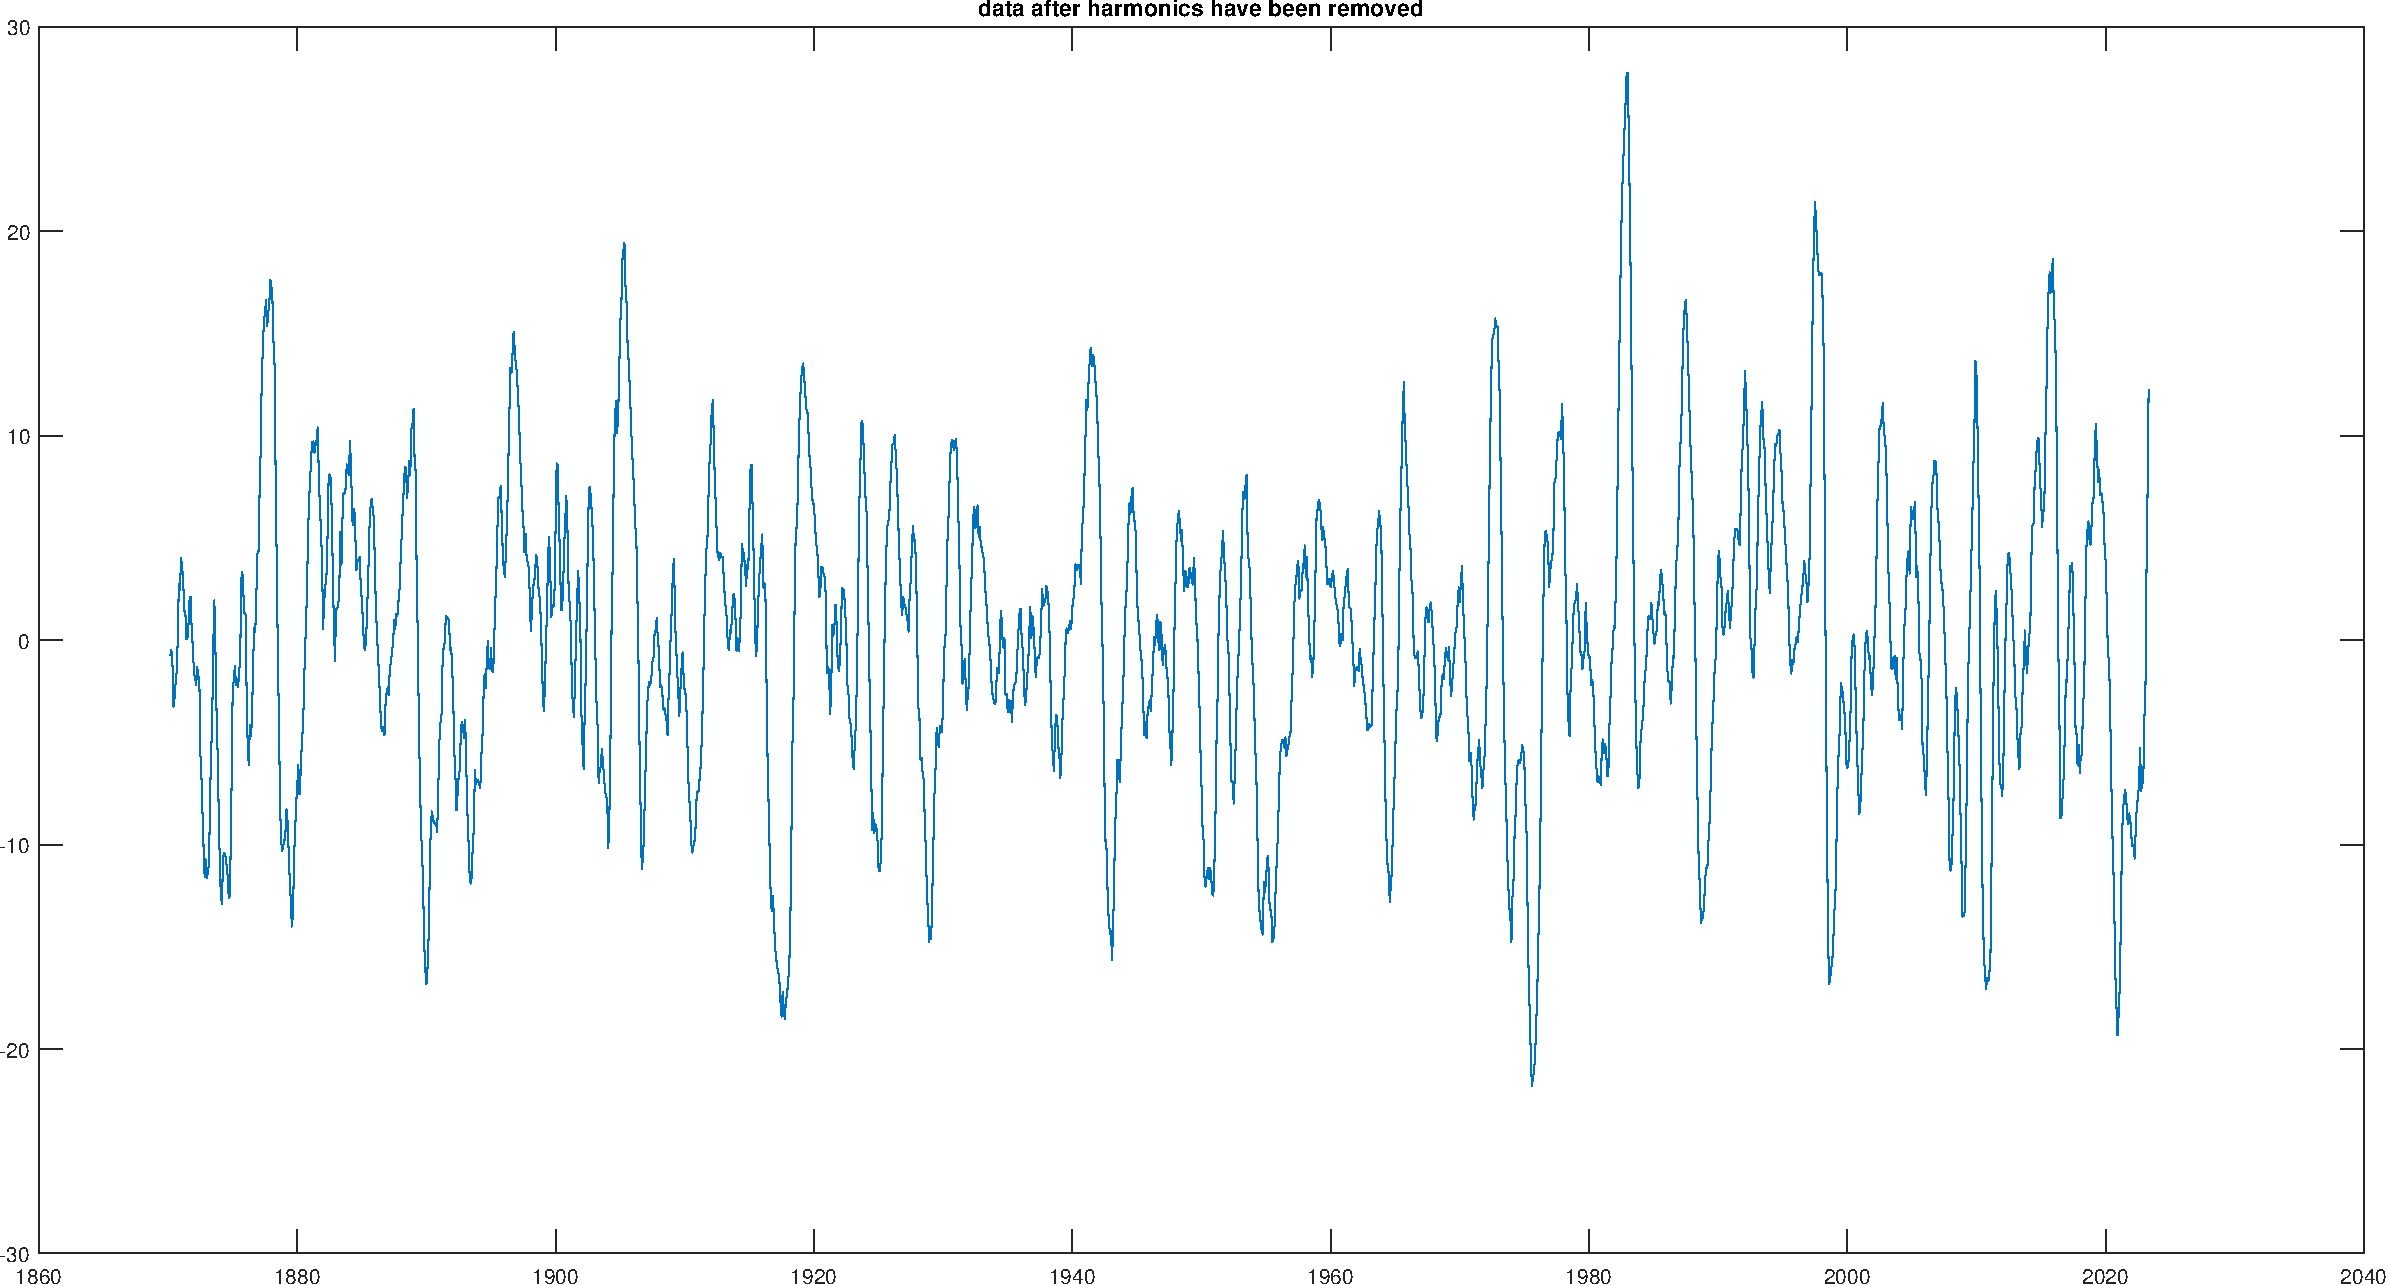
\includegraphics[width=1\linewidth]{inc/task2_del_harm}}
	\caption{Данные после удаления гармоник}
	\label{task2_del_harm}
\end{figure}

Подберем авторегрессию, сначала возьмем порядок 25 (рис. \ref{task2_predict_ar25}):
\begin{figure}[!h]
	\center{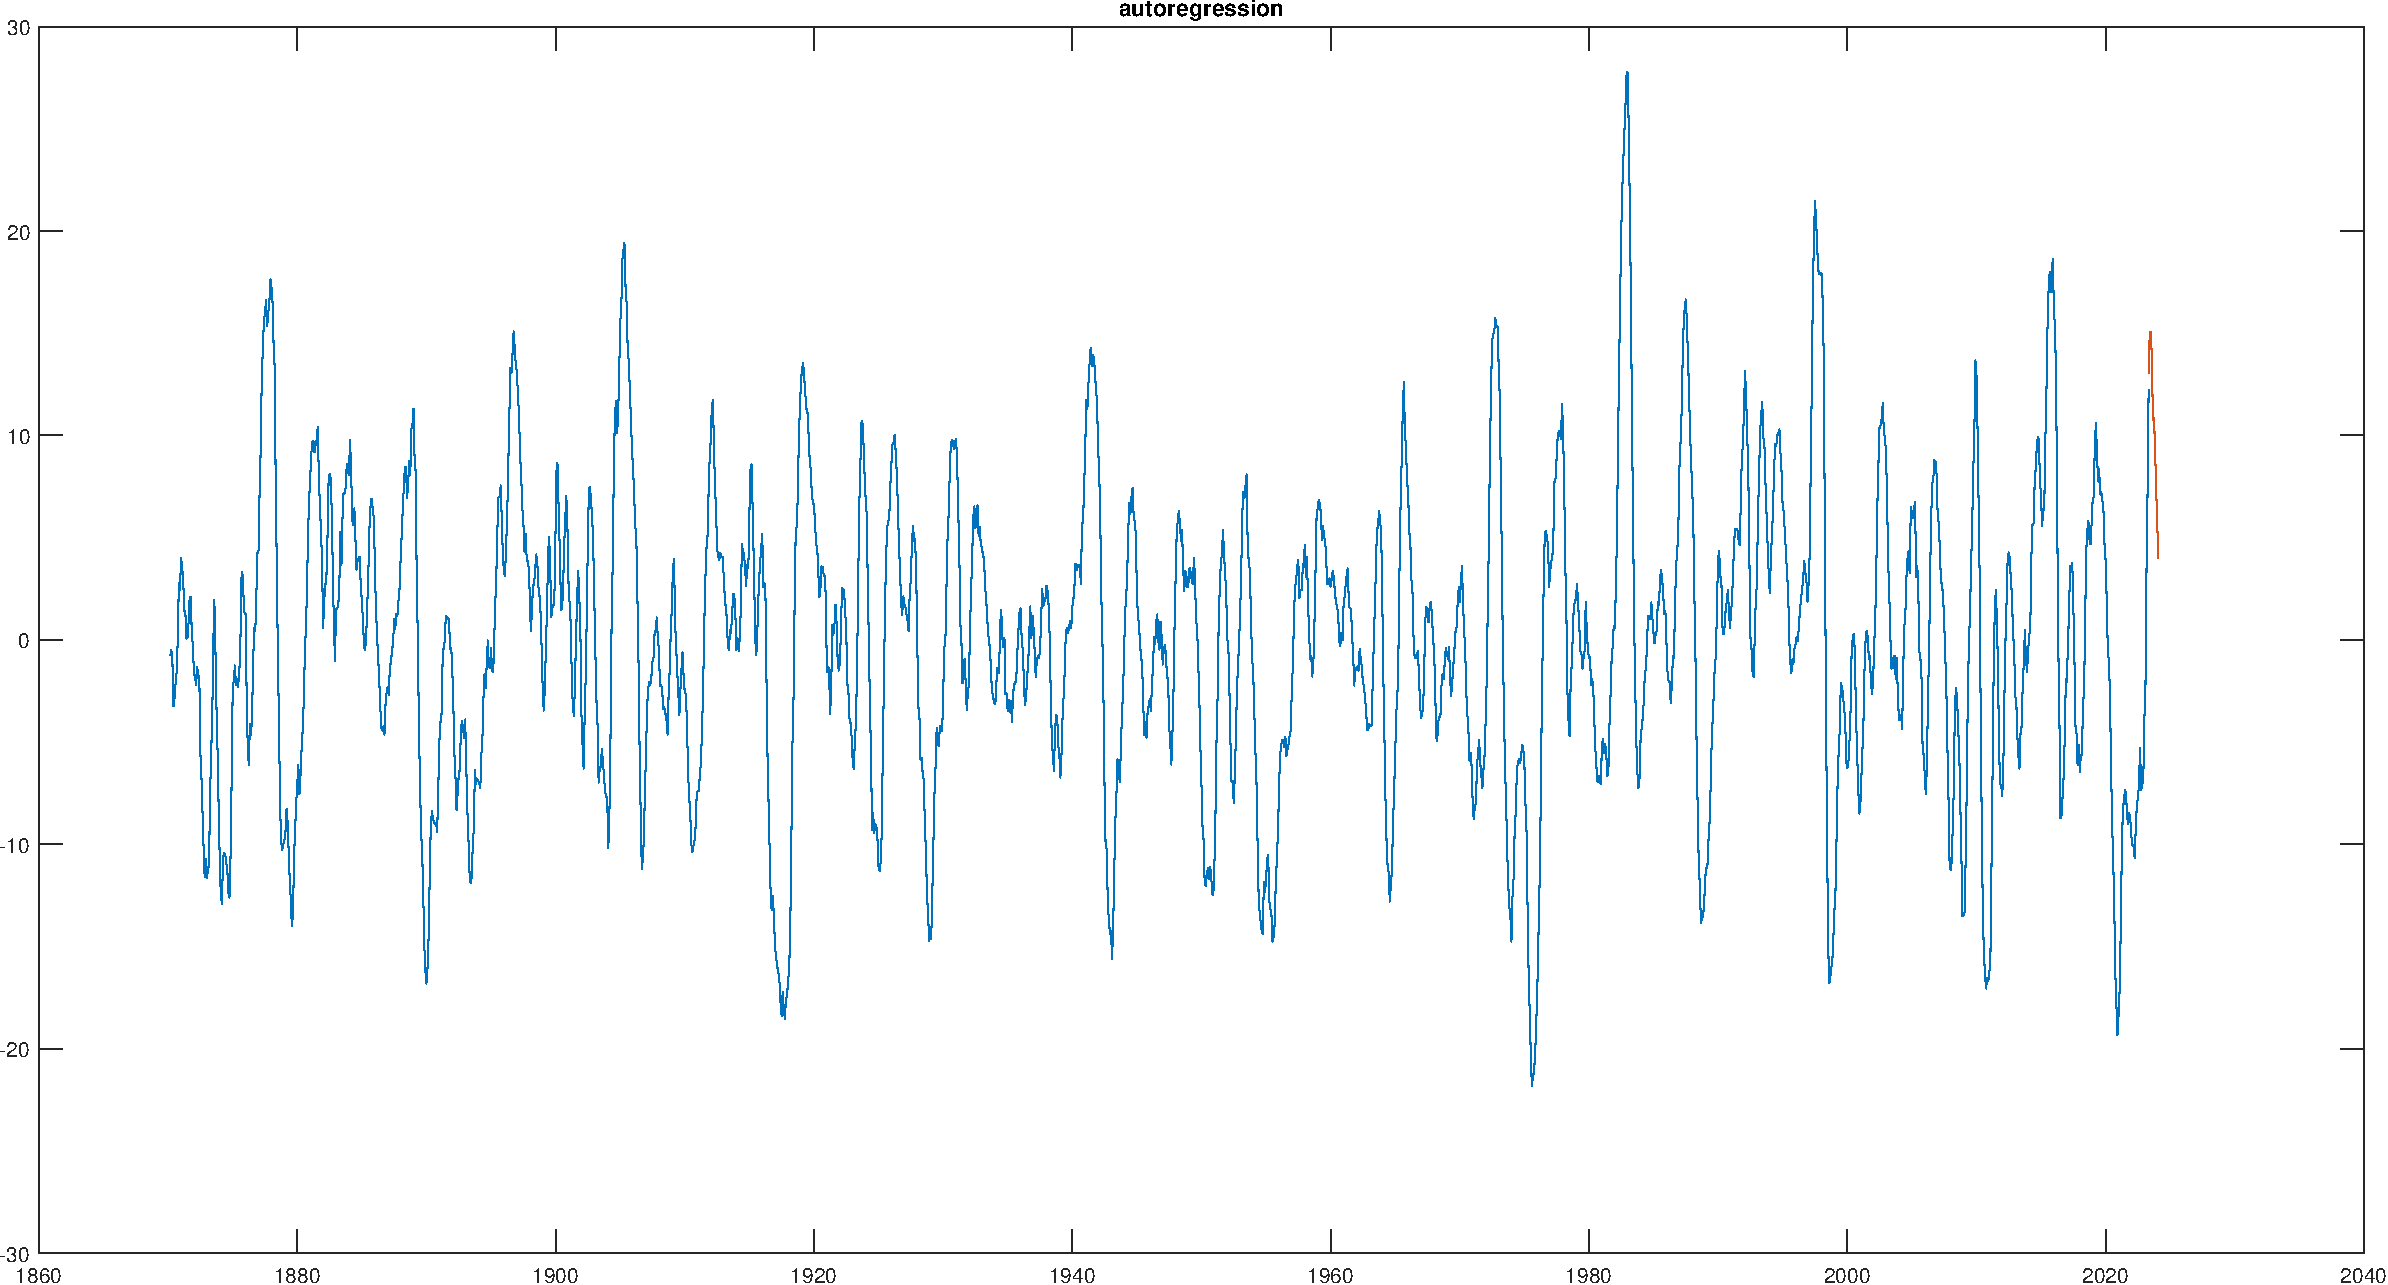
\includegraphics[width=1\linewidth]{inc/task2_predict_ar25}}
	\caption{Авторегрессия с порядком = 25}
	\label{task2_predict_ar25}
\end{figure}

Как видно по графику, при данном порядке авторегрессии через небольшой промежуток прогнозируется спад.

\newpage
Если же взять слишком маленький порядок, то график пойдет вверх (рис. \ref{task2_predict_ar3}):
\begin{figure}[!h]
	\center{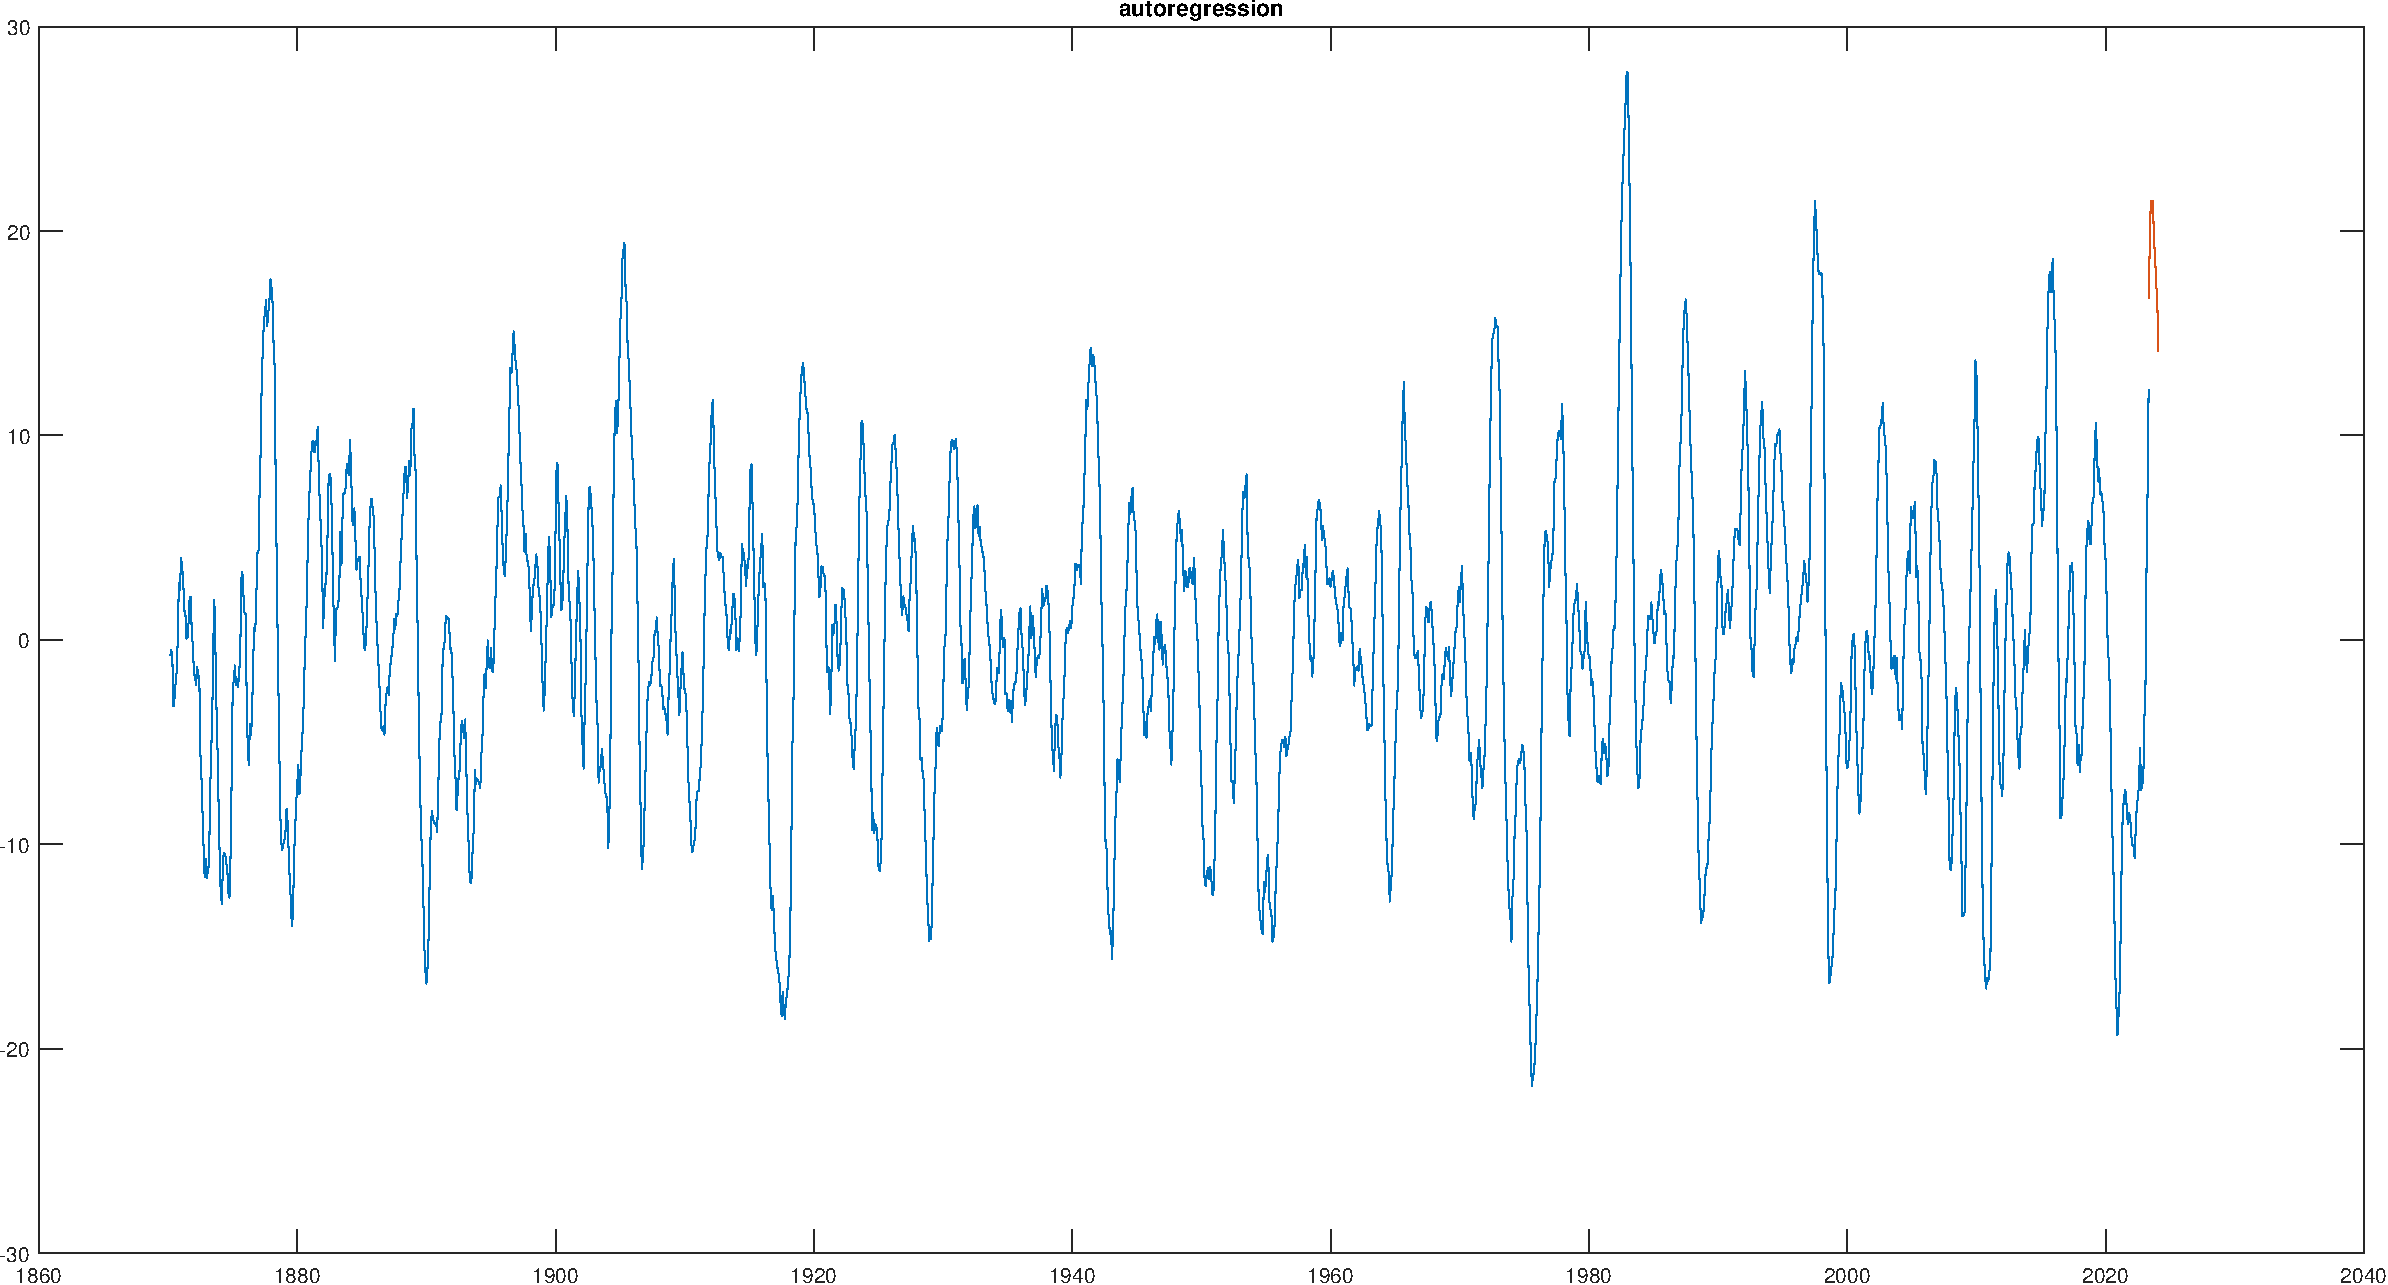
\includegraphics[width=1\linewidth]{inc/task2_predict_ar3}}
	\caption{Авторегрессия с порядком = 3}
	\label{task2_predict_ar3}
\end{figure}

Оставим порядок 25 и построим график прогноза (рис. \ref{task2_predict}):
\begin{figure}[!h]
	\center{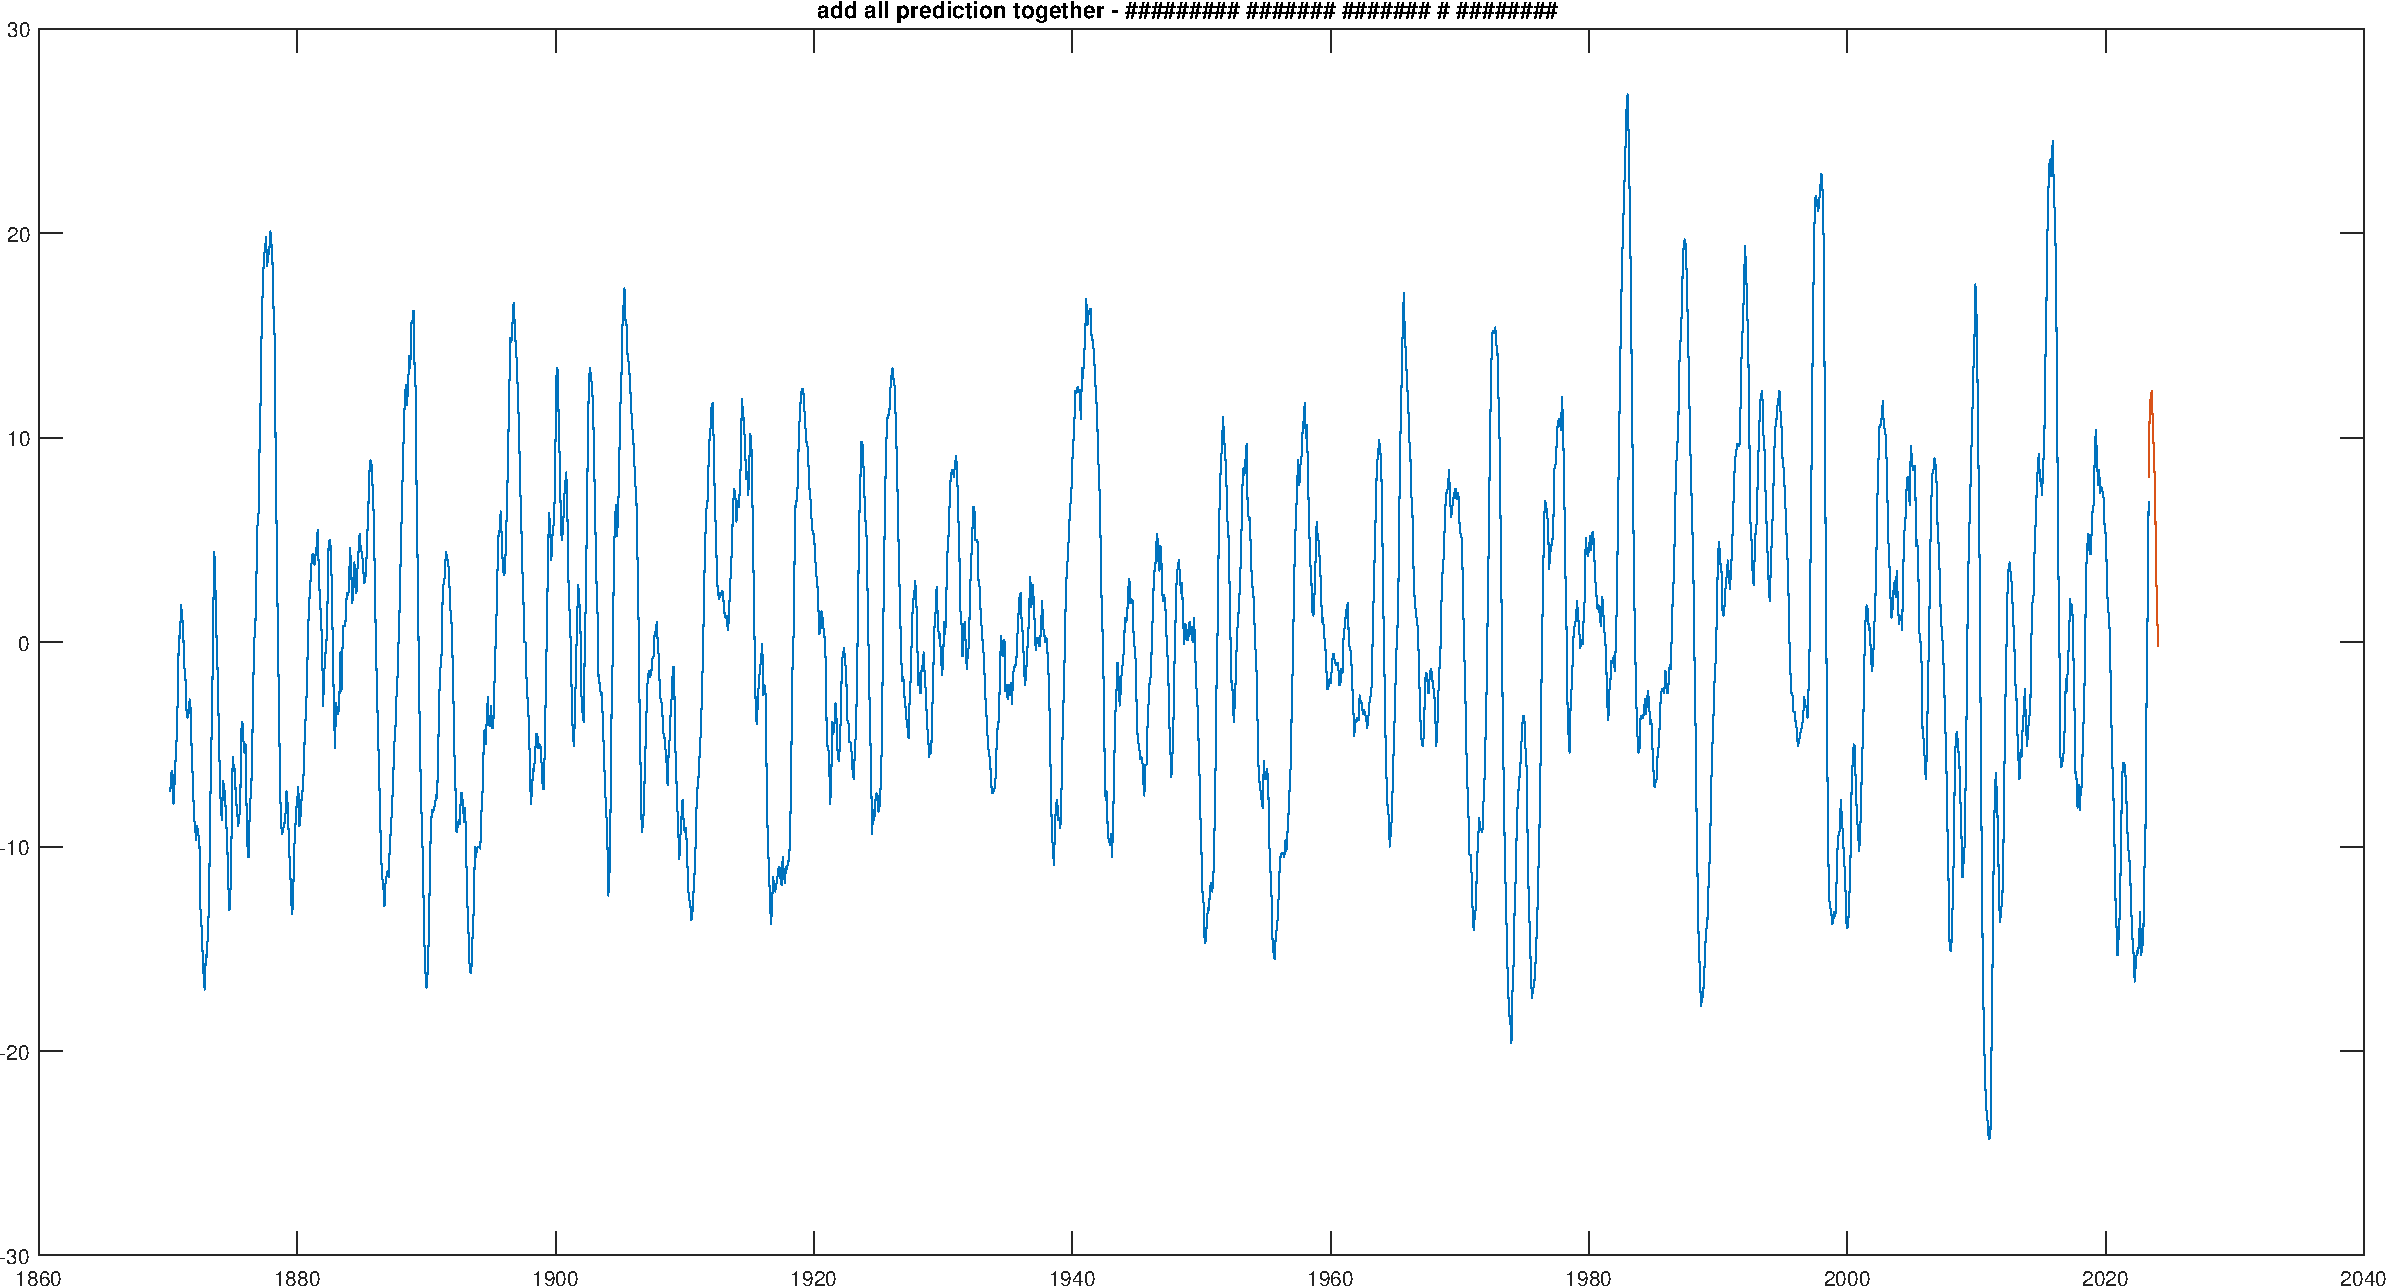
\includegraphics[width=1\linewidth]{inc/task2_predict}}
	\caption{График прогноза}
	\label{task2_predict}
\end{figure}

В итоге после небольшого подъема, по полученному прогнозу, ожидается спад.

\newpage
\textbf{Часть 3}

Повторим данный прогноз для сигнала из ЛР1 (рис. \ref{task3_signal}):
\begin{figure}[!h]
	\center{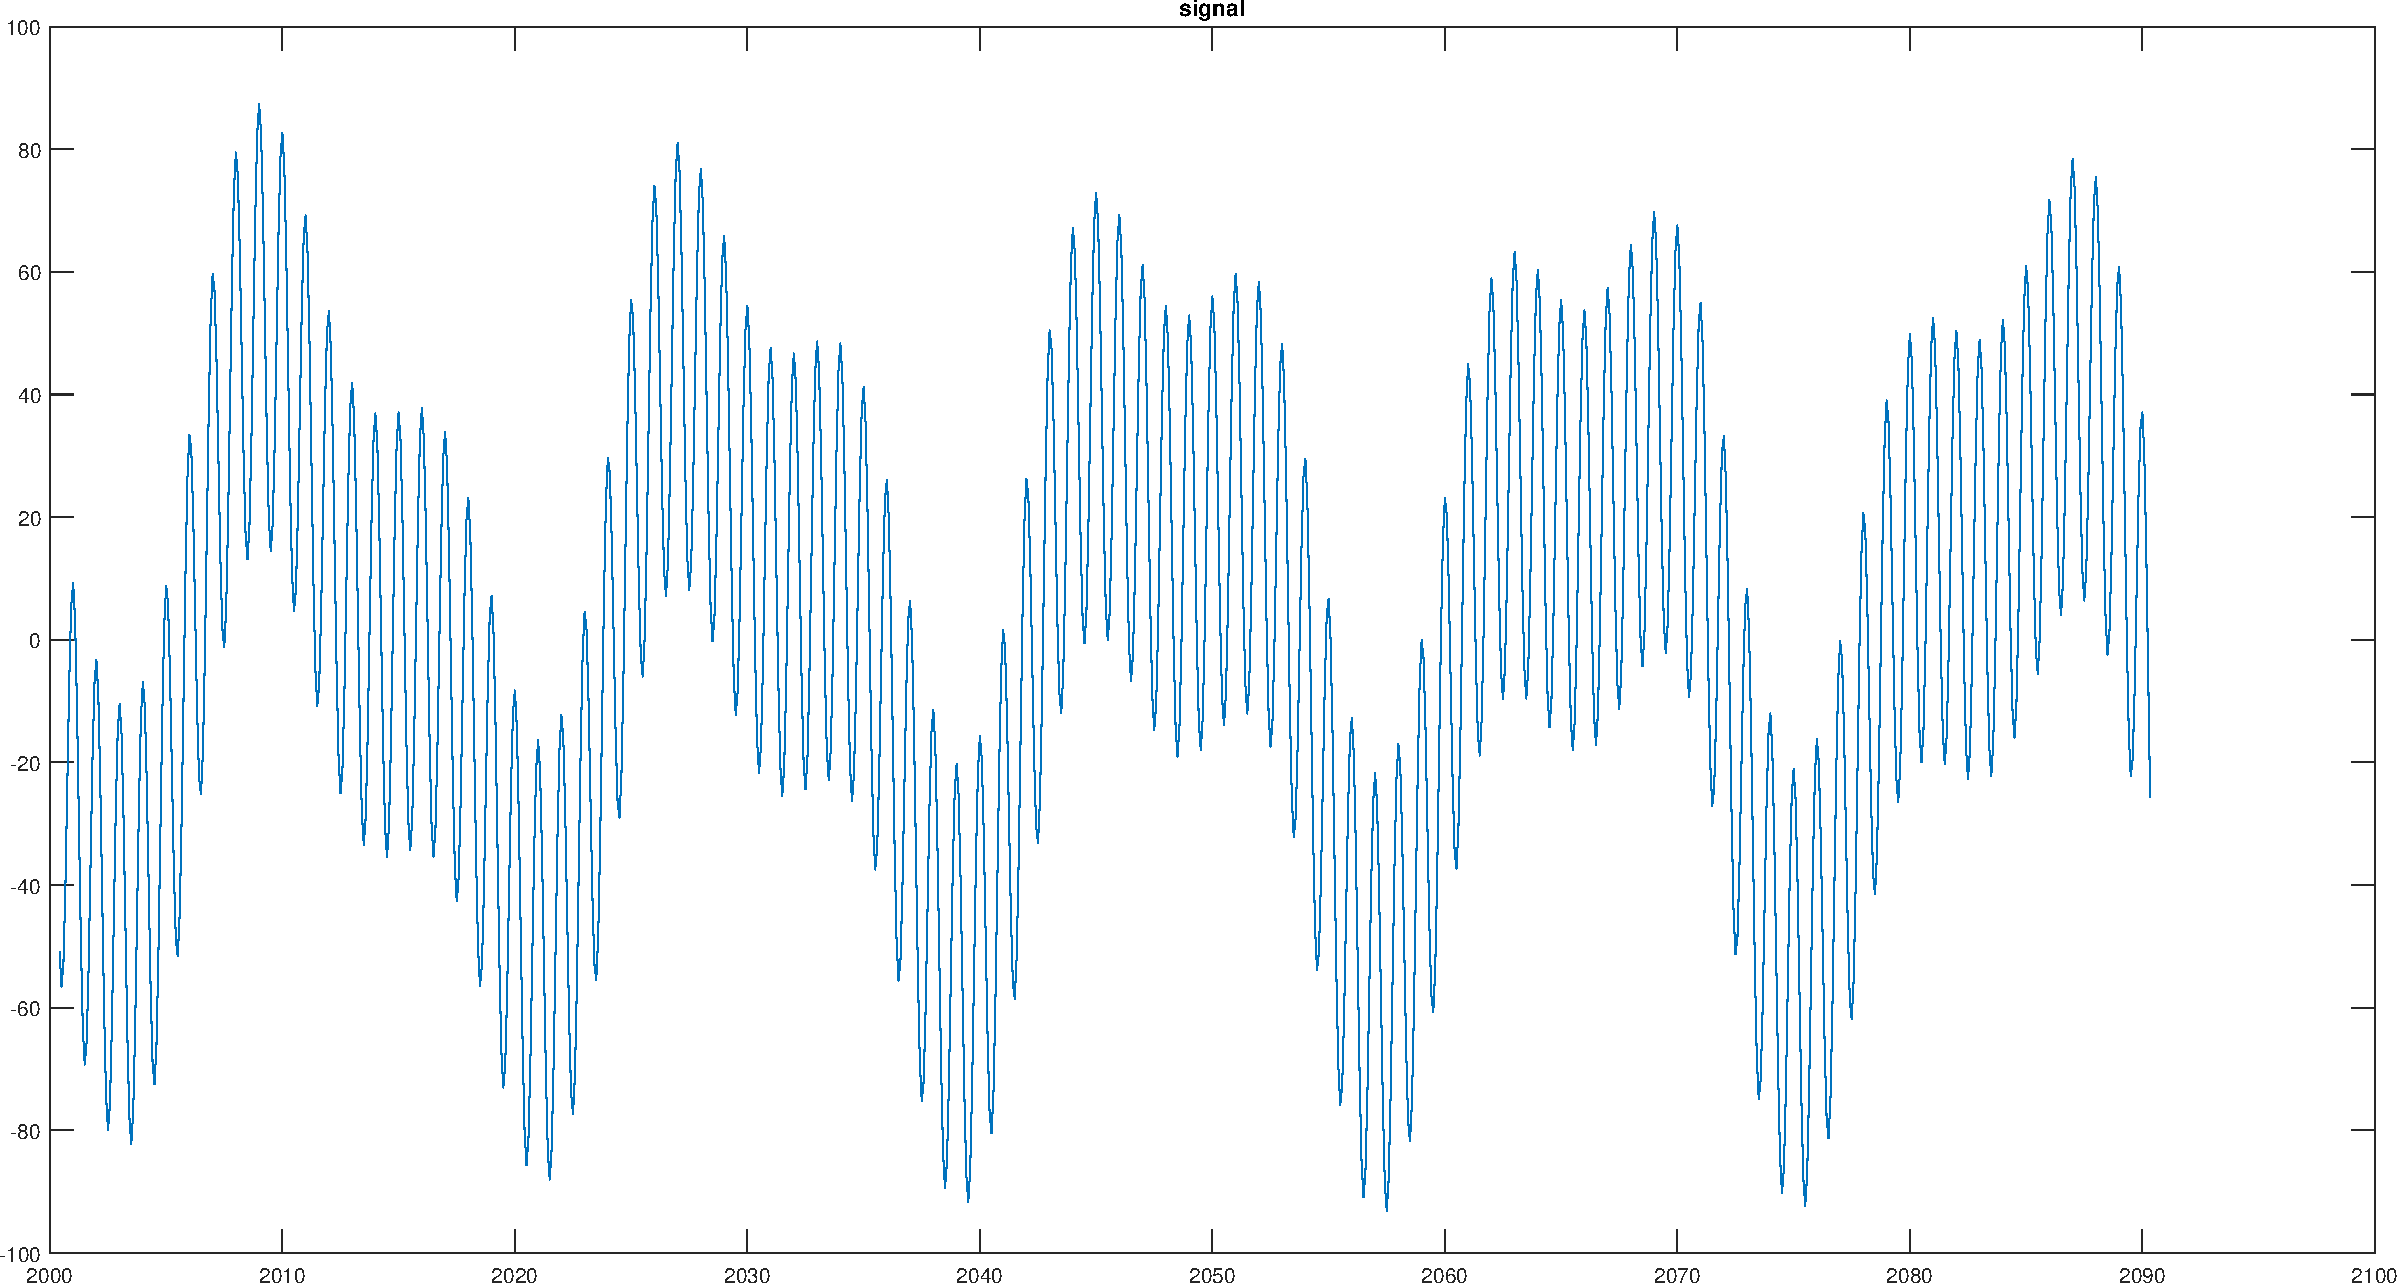
\includegraphics[width=1\linewidth]{inc/task3_signal}}
	\caption{Сигнал из ЛР1}
	\label{task3_signal}
\end{figure}

Добавим к нему цветной шум (рис. \ref{task3_noise}-\ref{task3_signal_noise}):
\begin{figure}[!h]
	\center{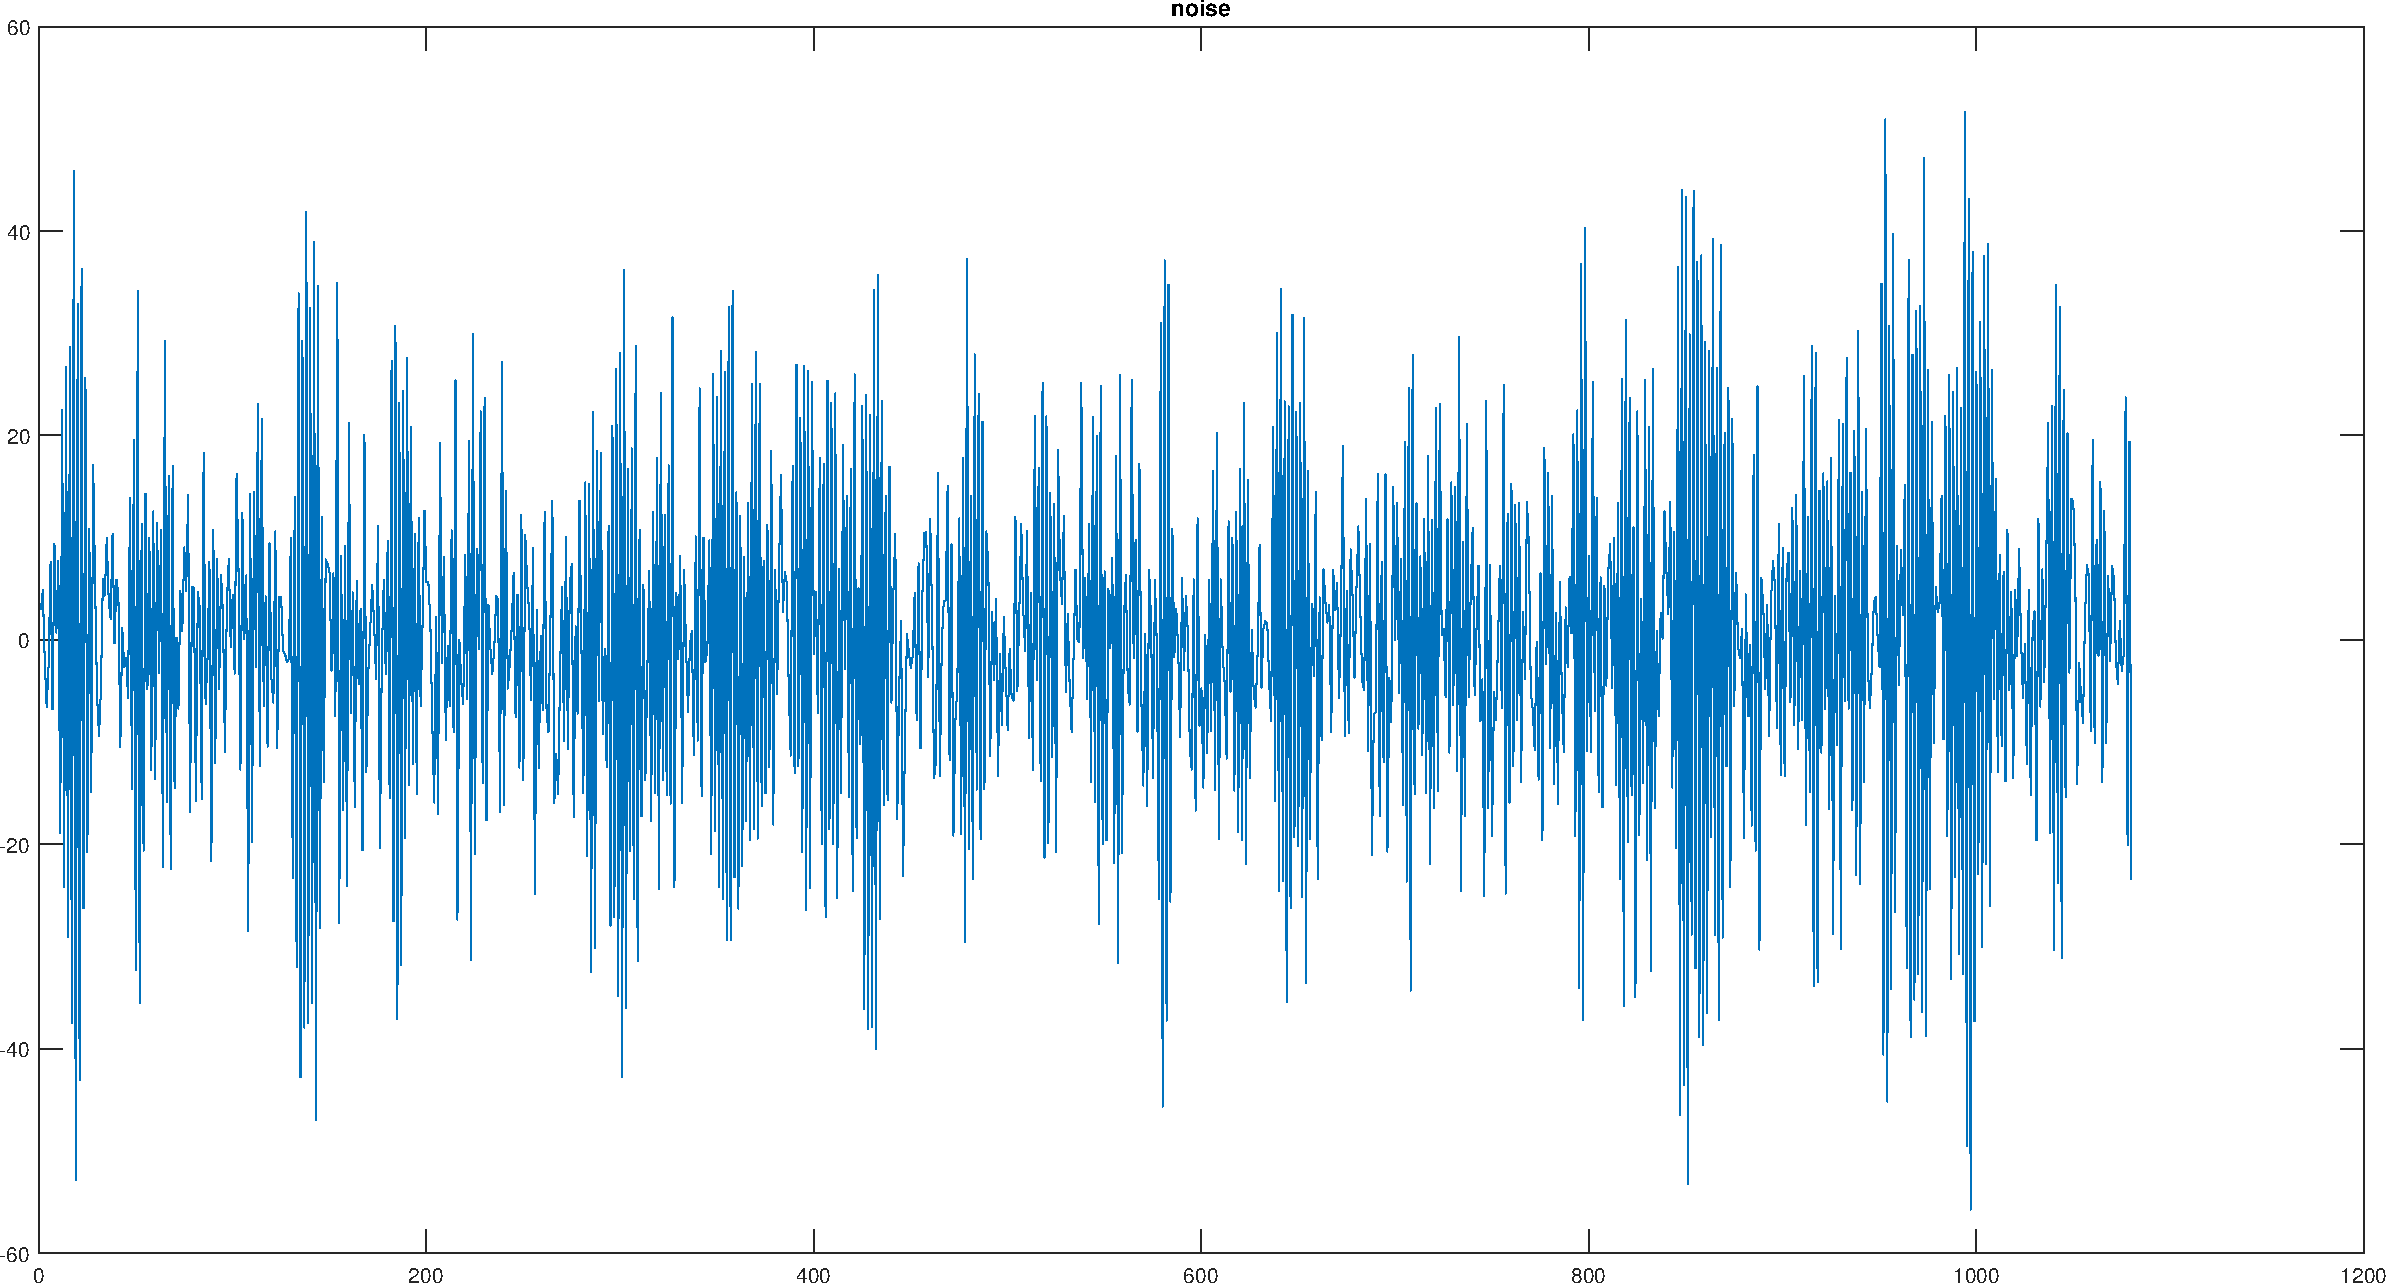
\includegraphics[width=1\linewidth]{inc/task3_noise}}
	\caption{Цветной шум}
	\label{task3_noise}
\end{figure}

\newpage
\begin{figure}[!h]
	\center{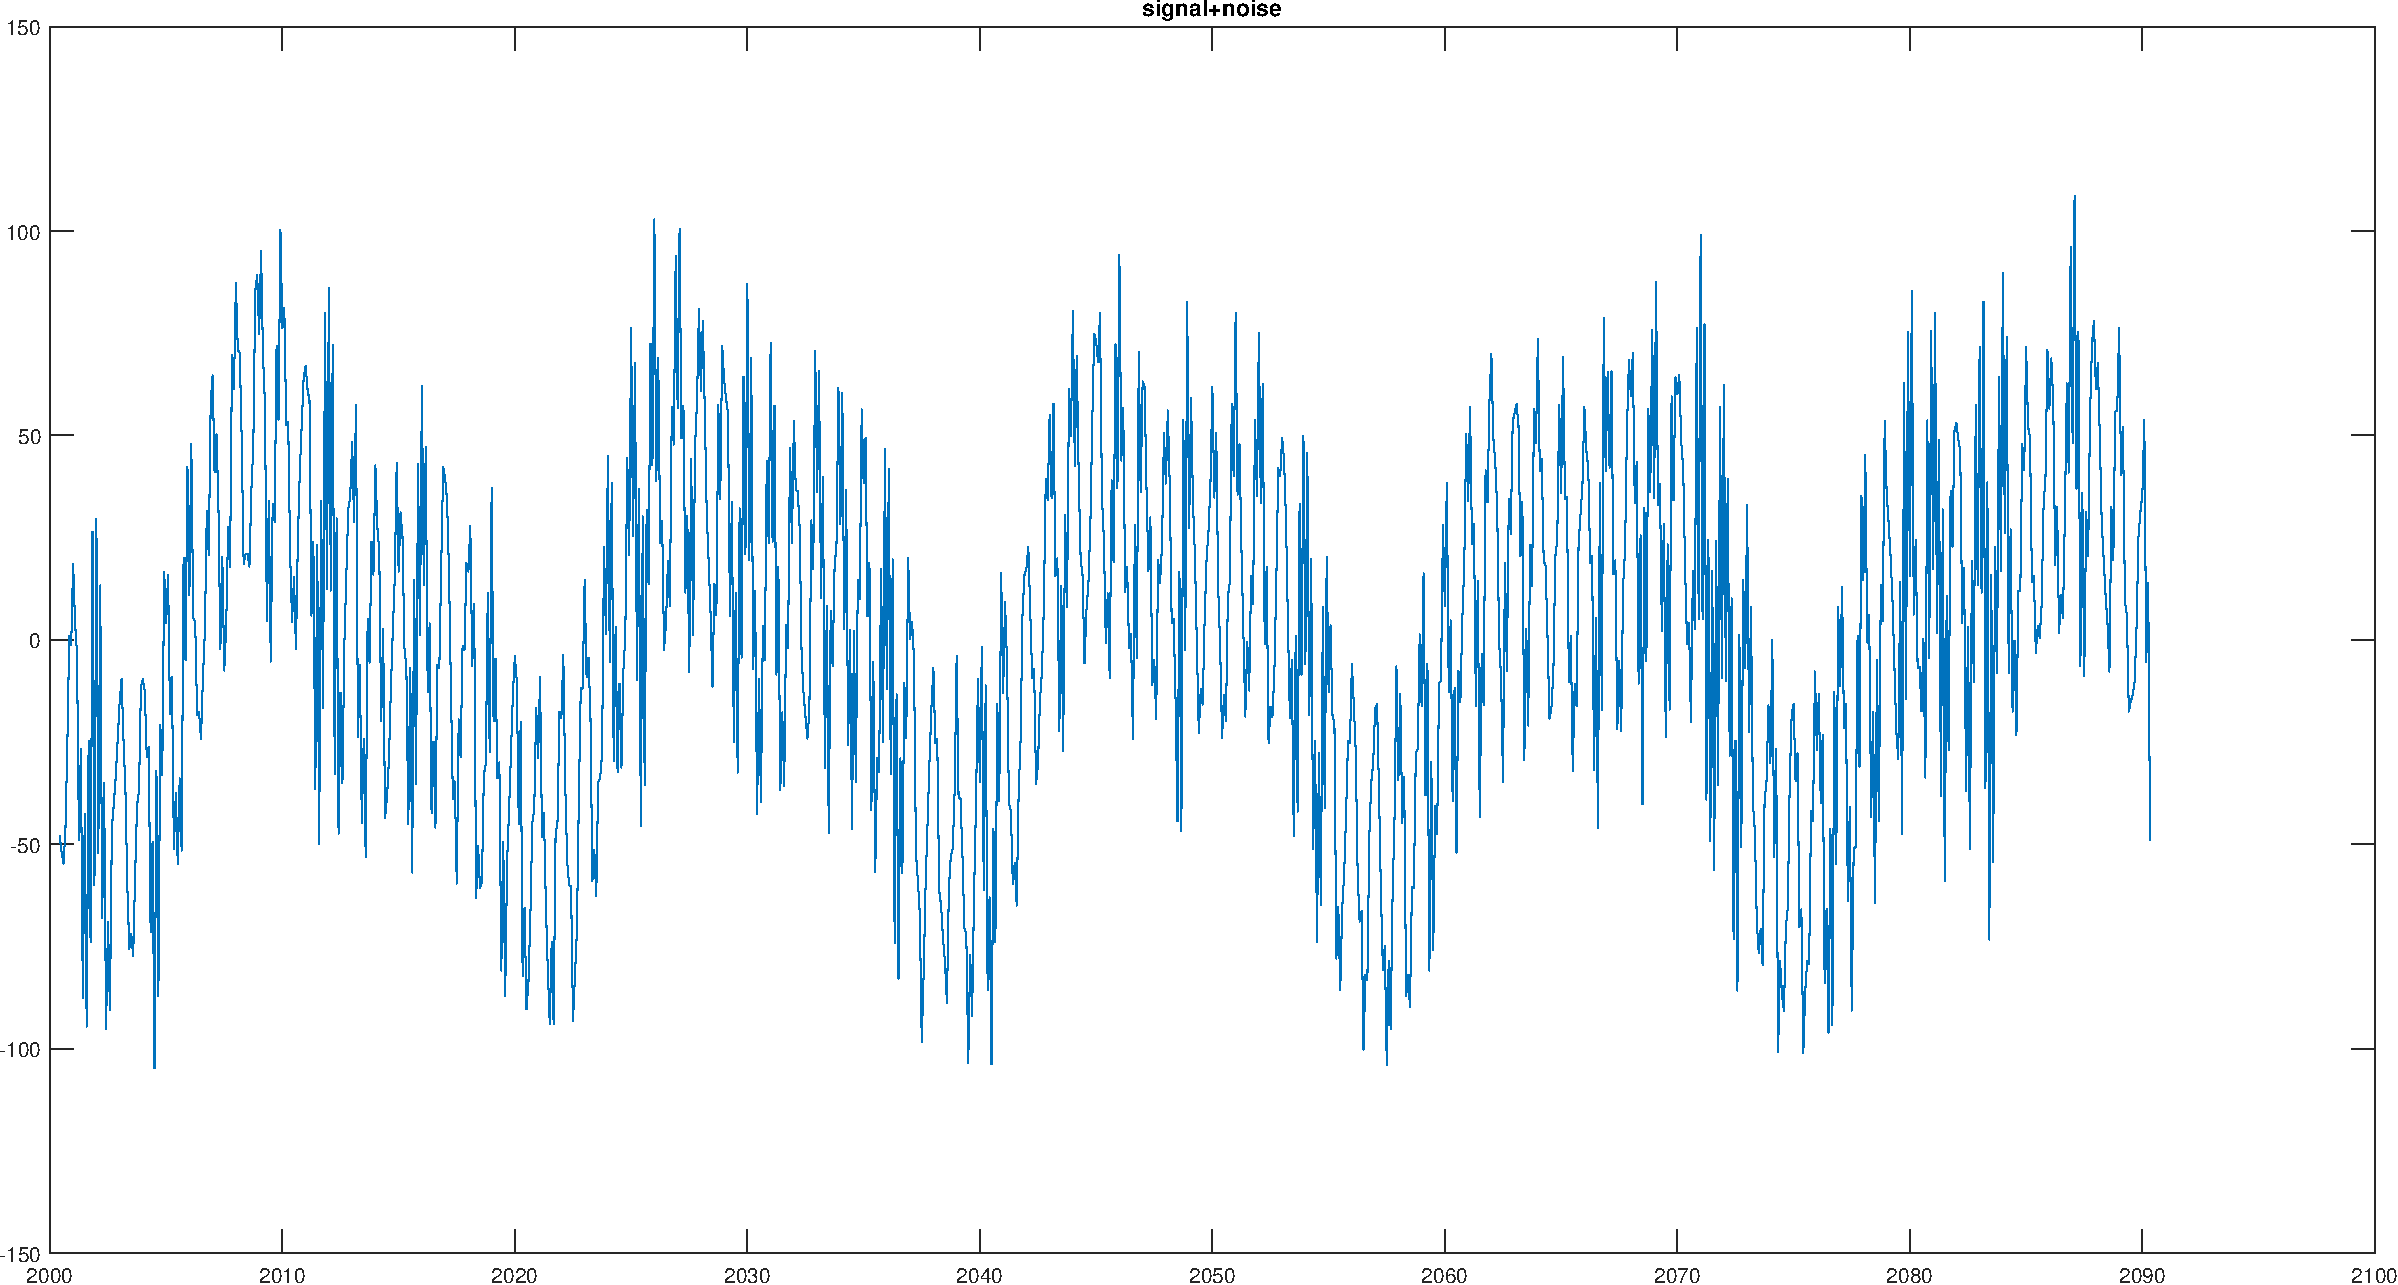
\includegraphics[width=1\linewidth]{inc/task3_signal_noise}}
	\caption{Сигнал с шумом}
	\label{task3_signal_noise}
\end{figure}

Вычислим смещенную и несмещенную оценку АКФ (рис. \ref{task3_acf_biased}-\ref{task3_acf_unbiased}):
\begin{figure}[!h]
	\center{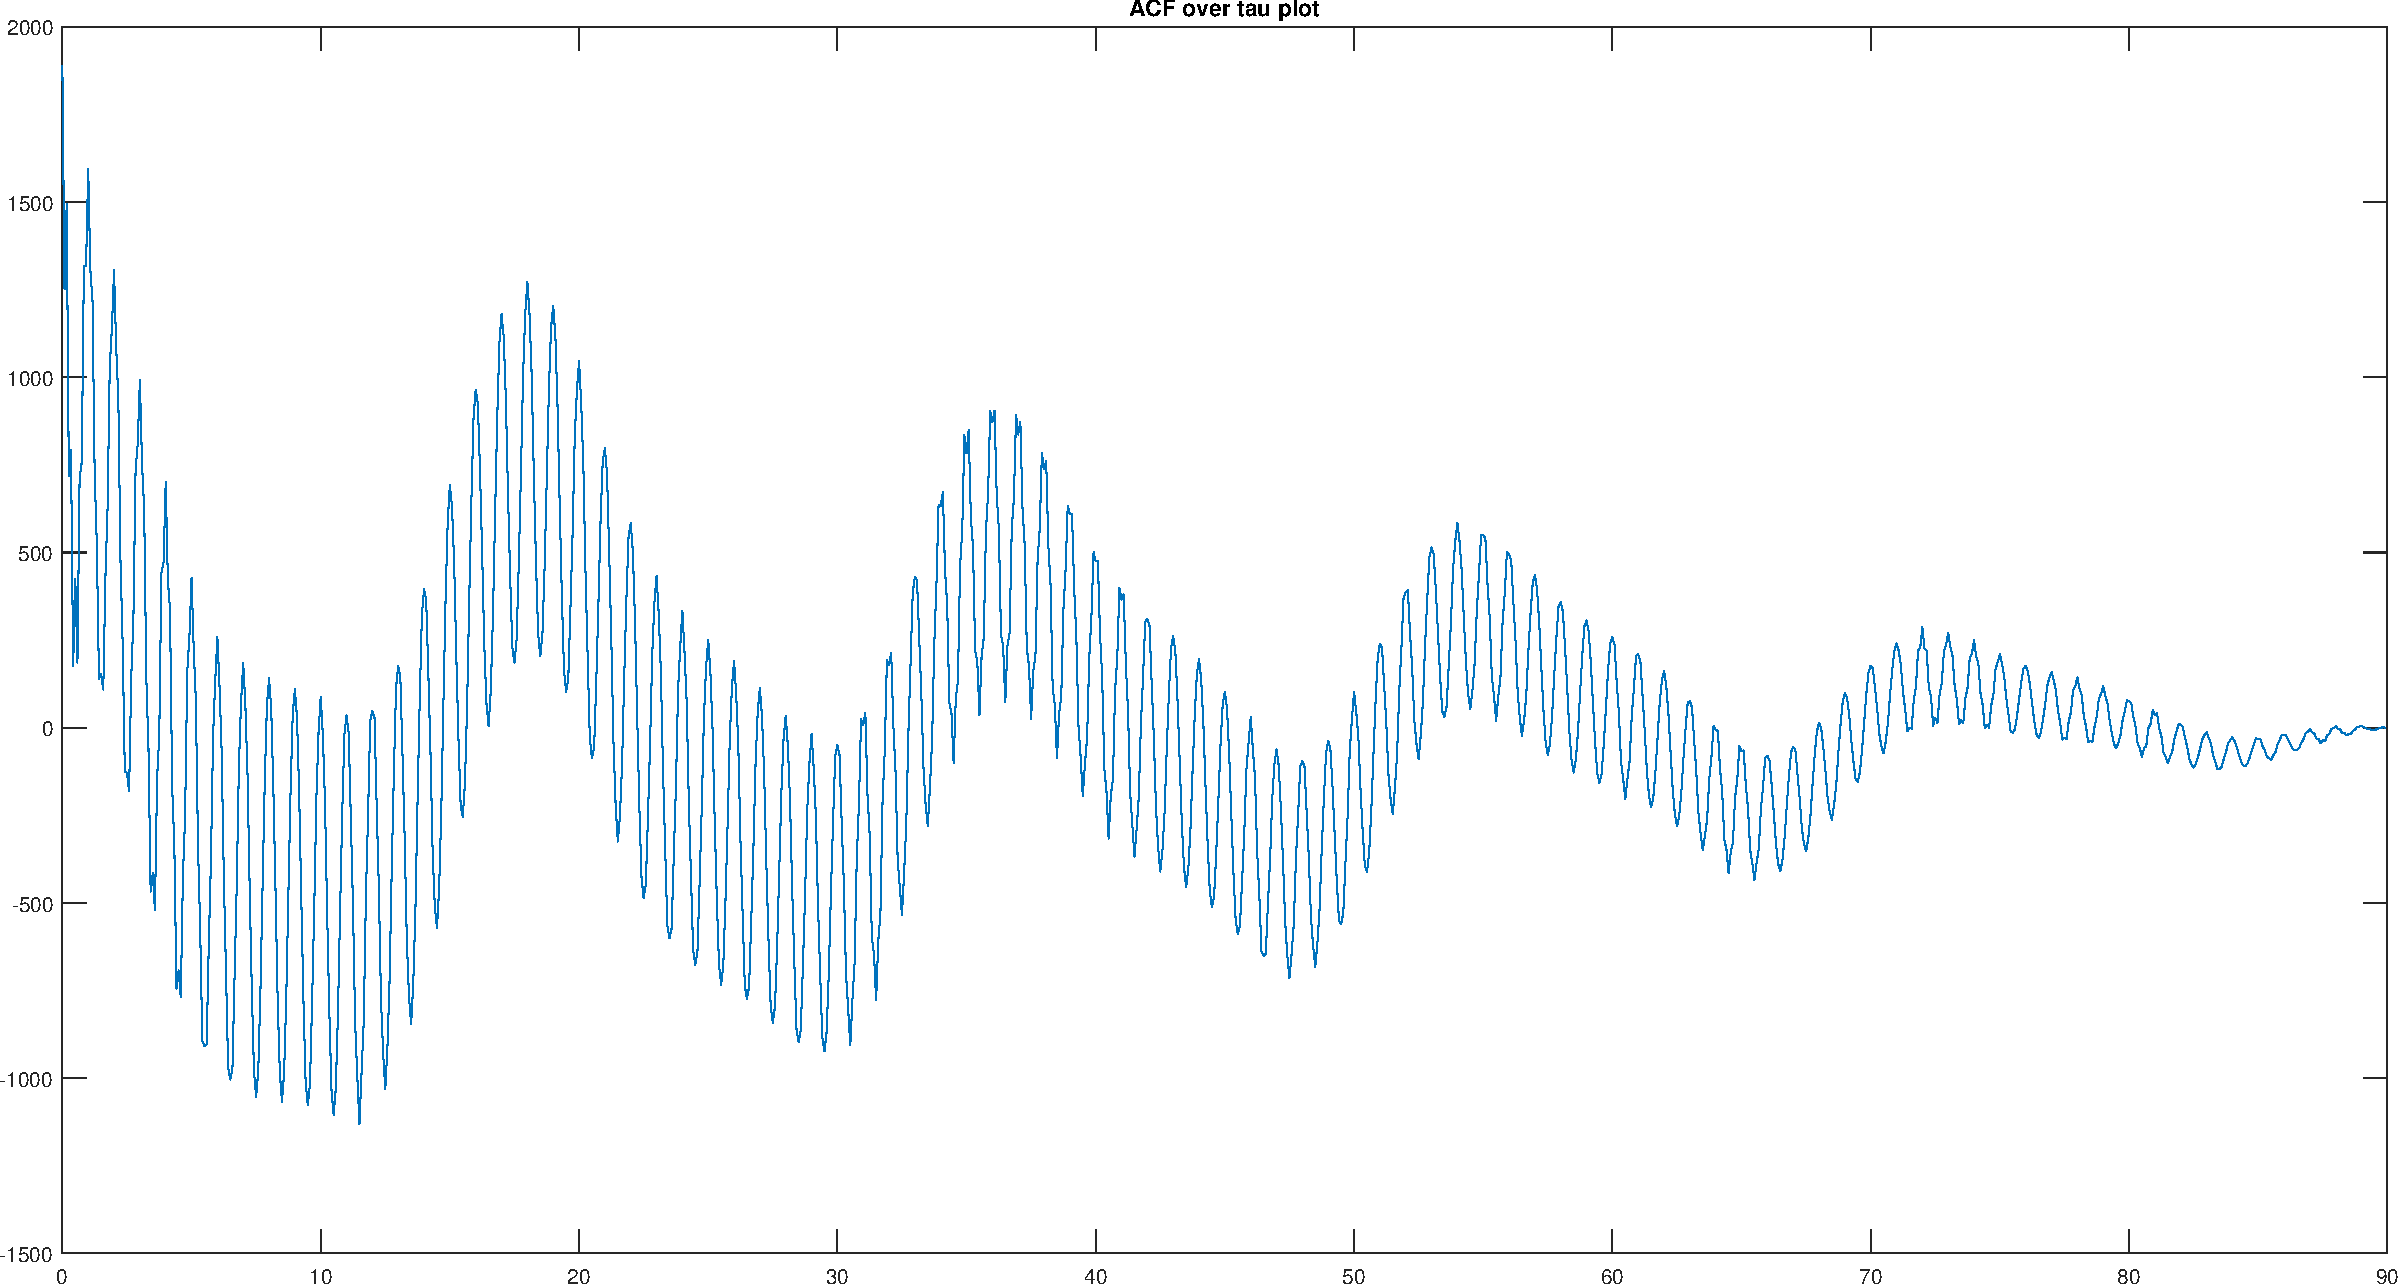
\includegraphics[width=1\linewidth]{inc/task3_acf_biased}}
	\caption{Cмещенная АКФ}
	\label{task3_acf_biased}
\end{figure}

\newpage
\begin{figure}[!h]
	\center{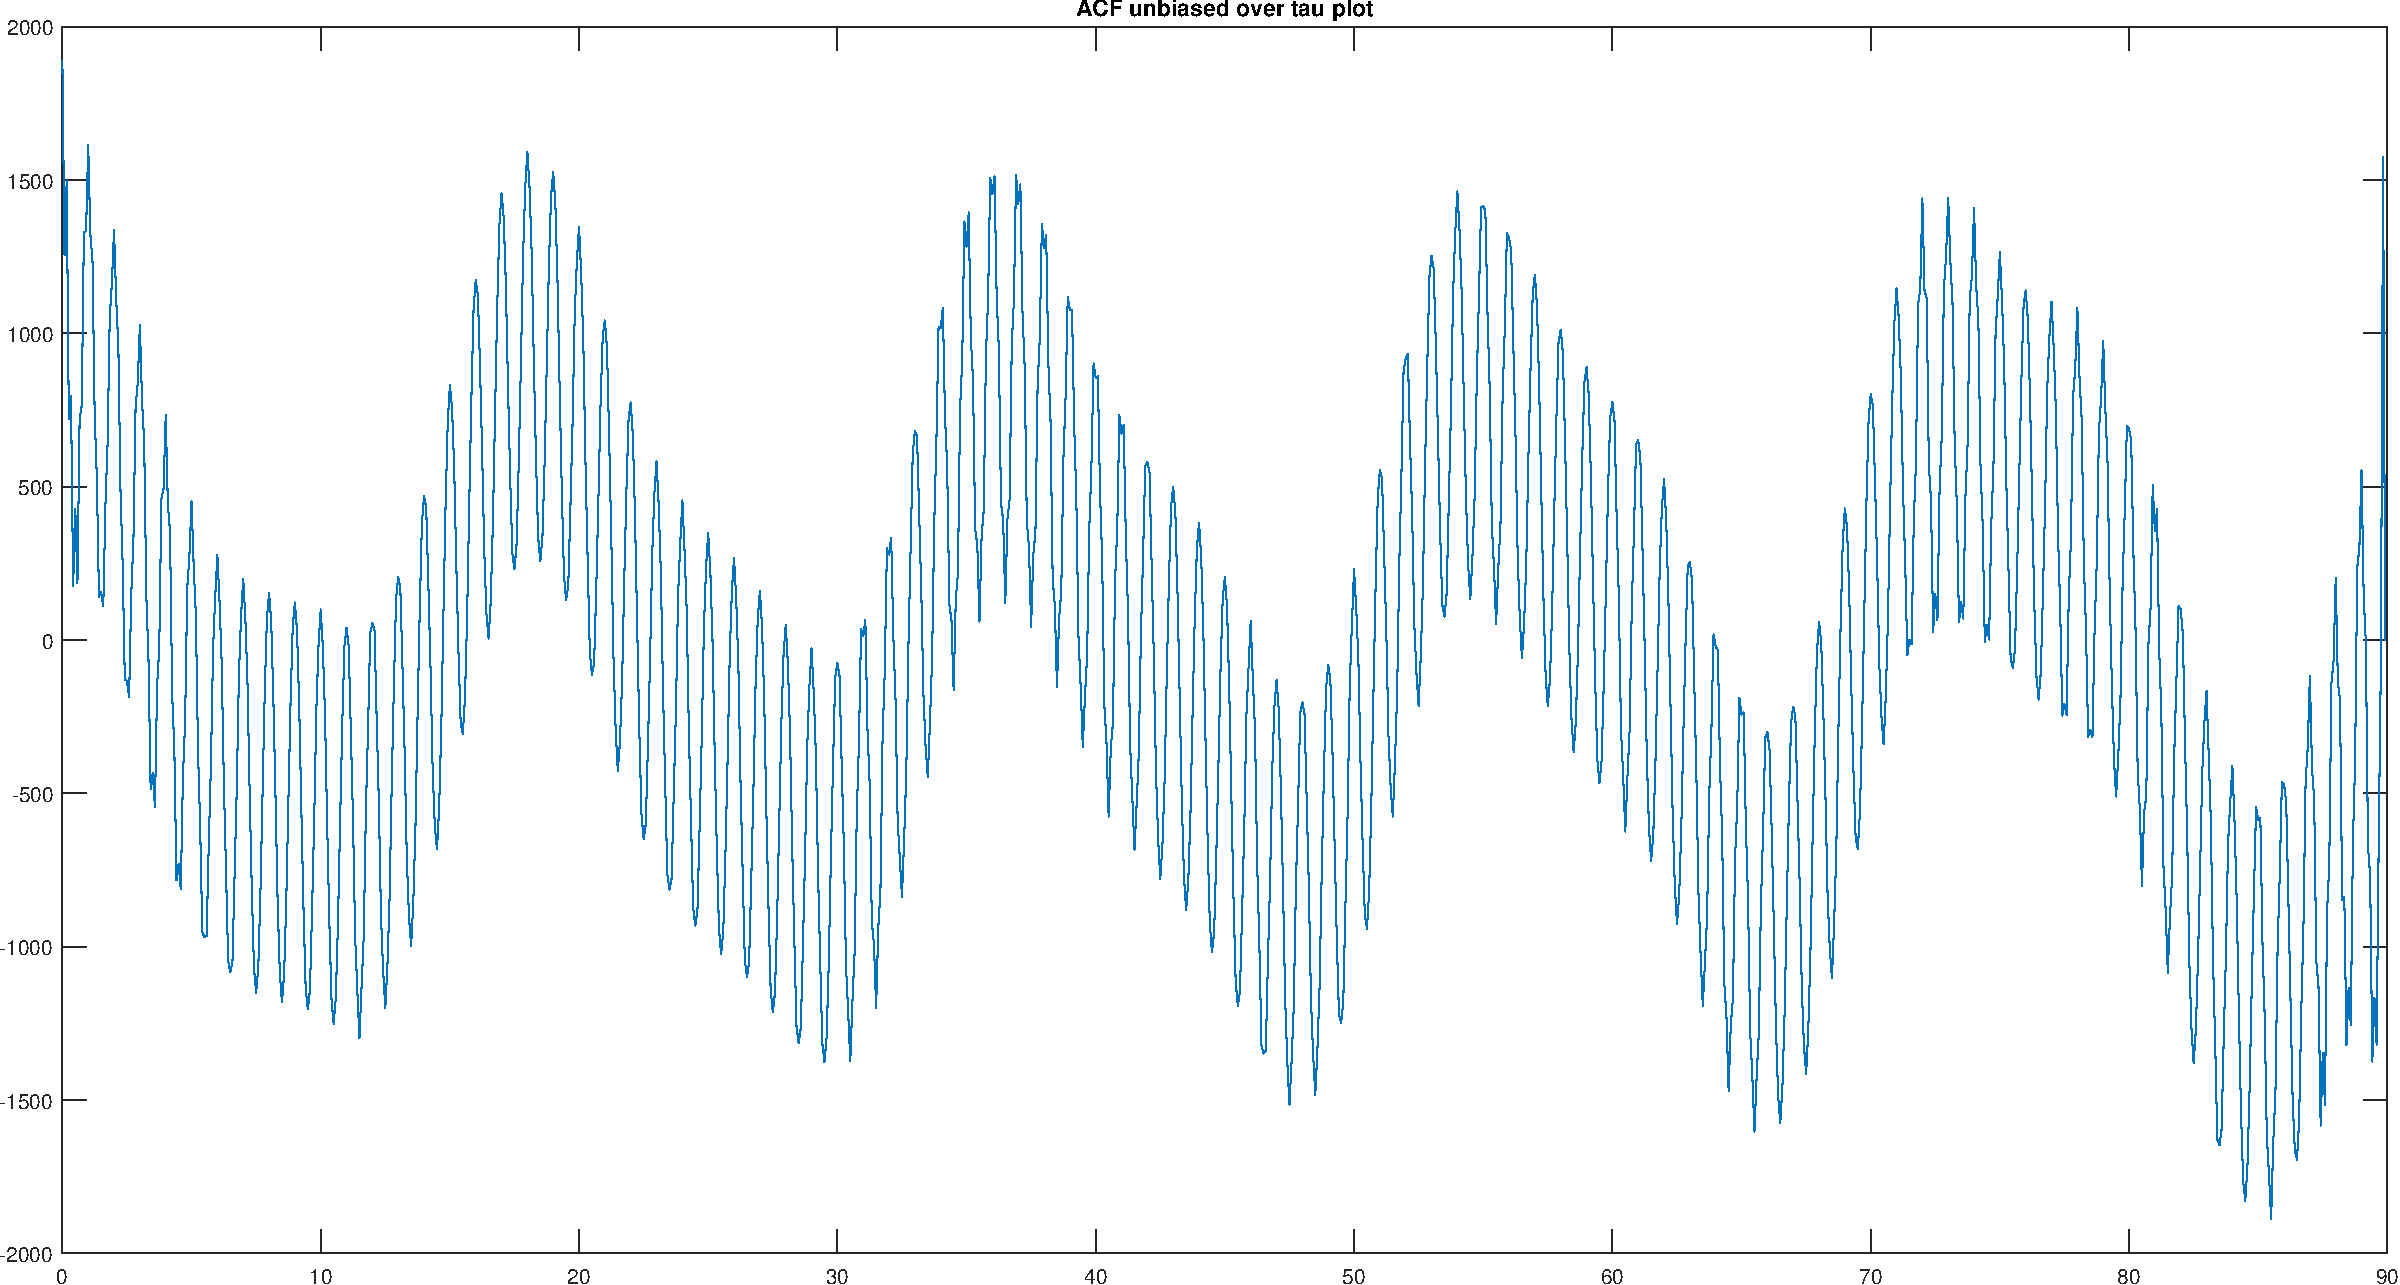
\includegraphics[width=1\linewidth]{inc/task3_acf_unbiased}}
	\caption{Несмещенная АКФ}
	\label{task3_acf_unbiased}
\end{figure}

Построим спектральную плотность для периодов (рис. \ref{task3_psd_periods}):
\begin{figure}[!h]
	\center{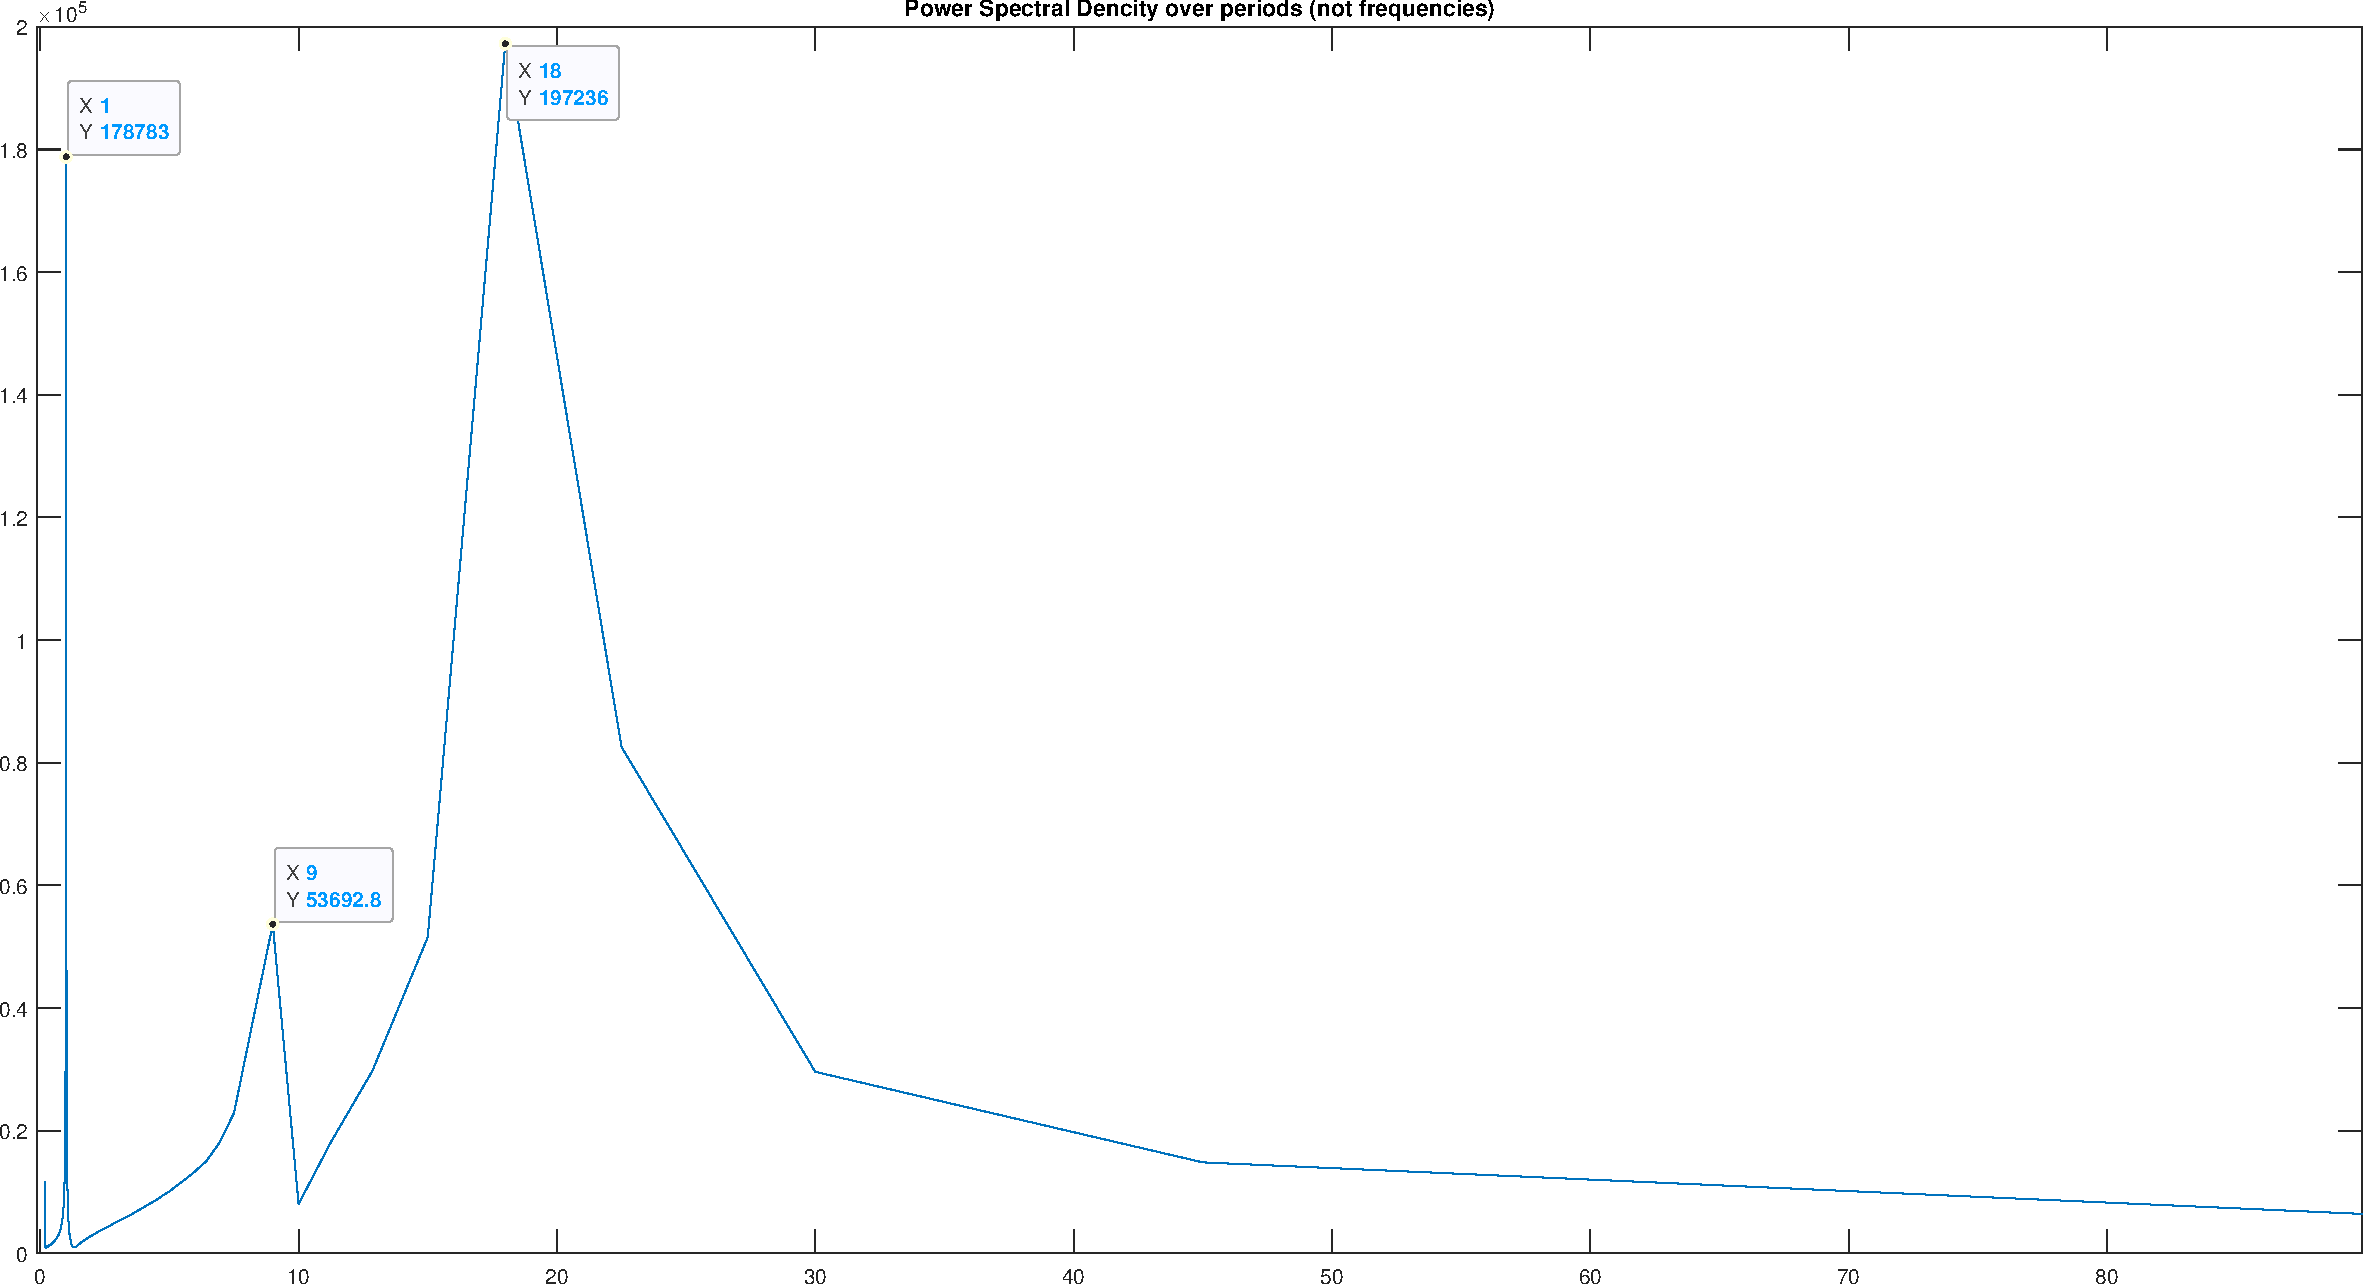
\includegraphics[width=1\linewidth]{inc/task3_psd_periods}}
	\caption{СПМ для периодов}
	\label{task3_psd_periods}
\end{figure}


\newpage
Подберем полиномиальную модель (возьмем порядок 2) и определим тренд (рис. \ref{task3_predict_poly}):
\begin{figure}[!h]
	\center{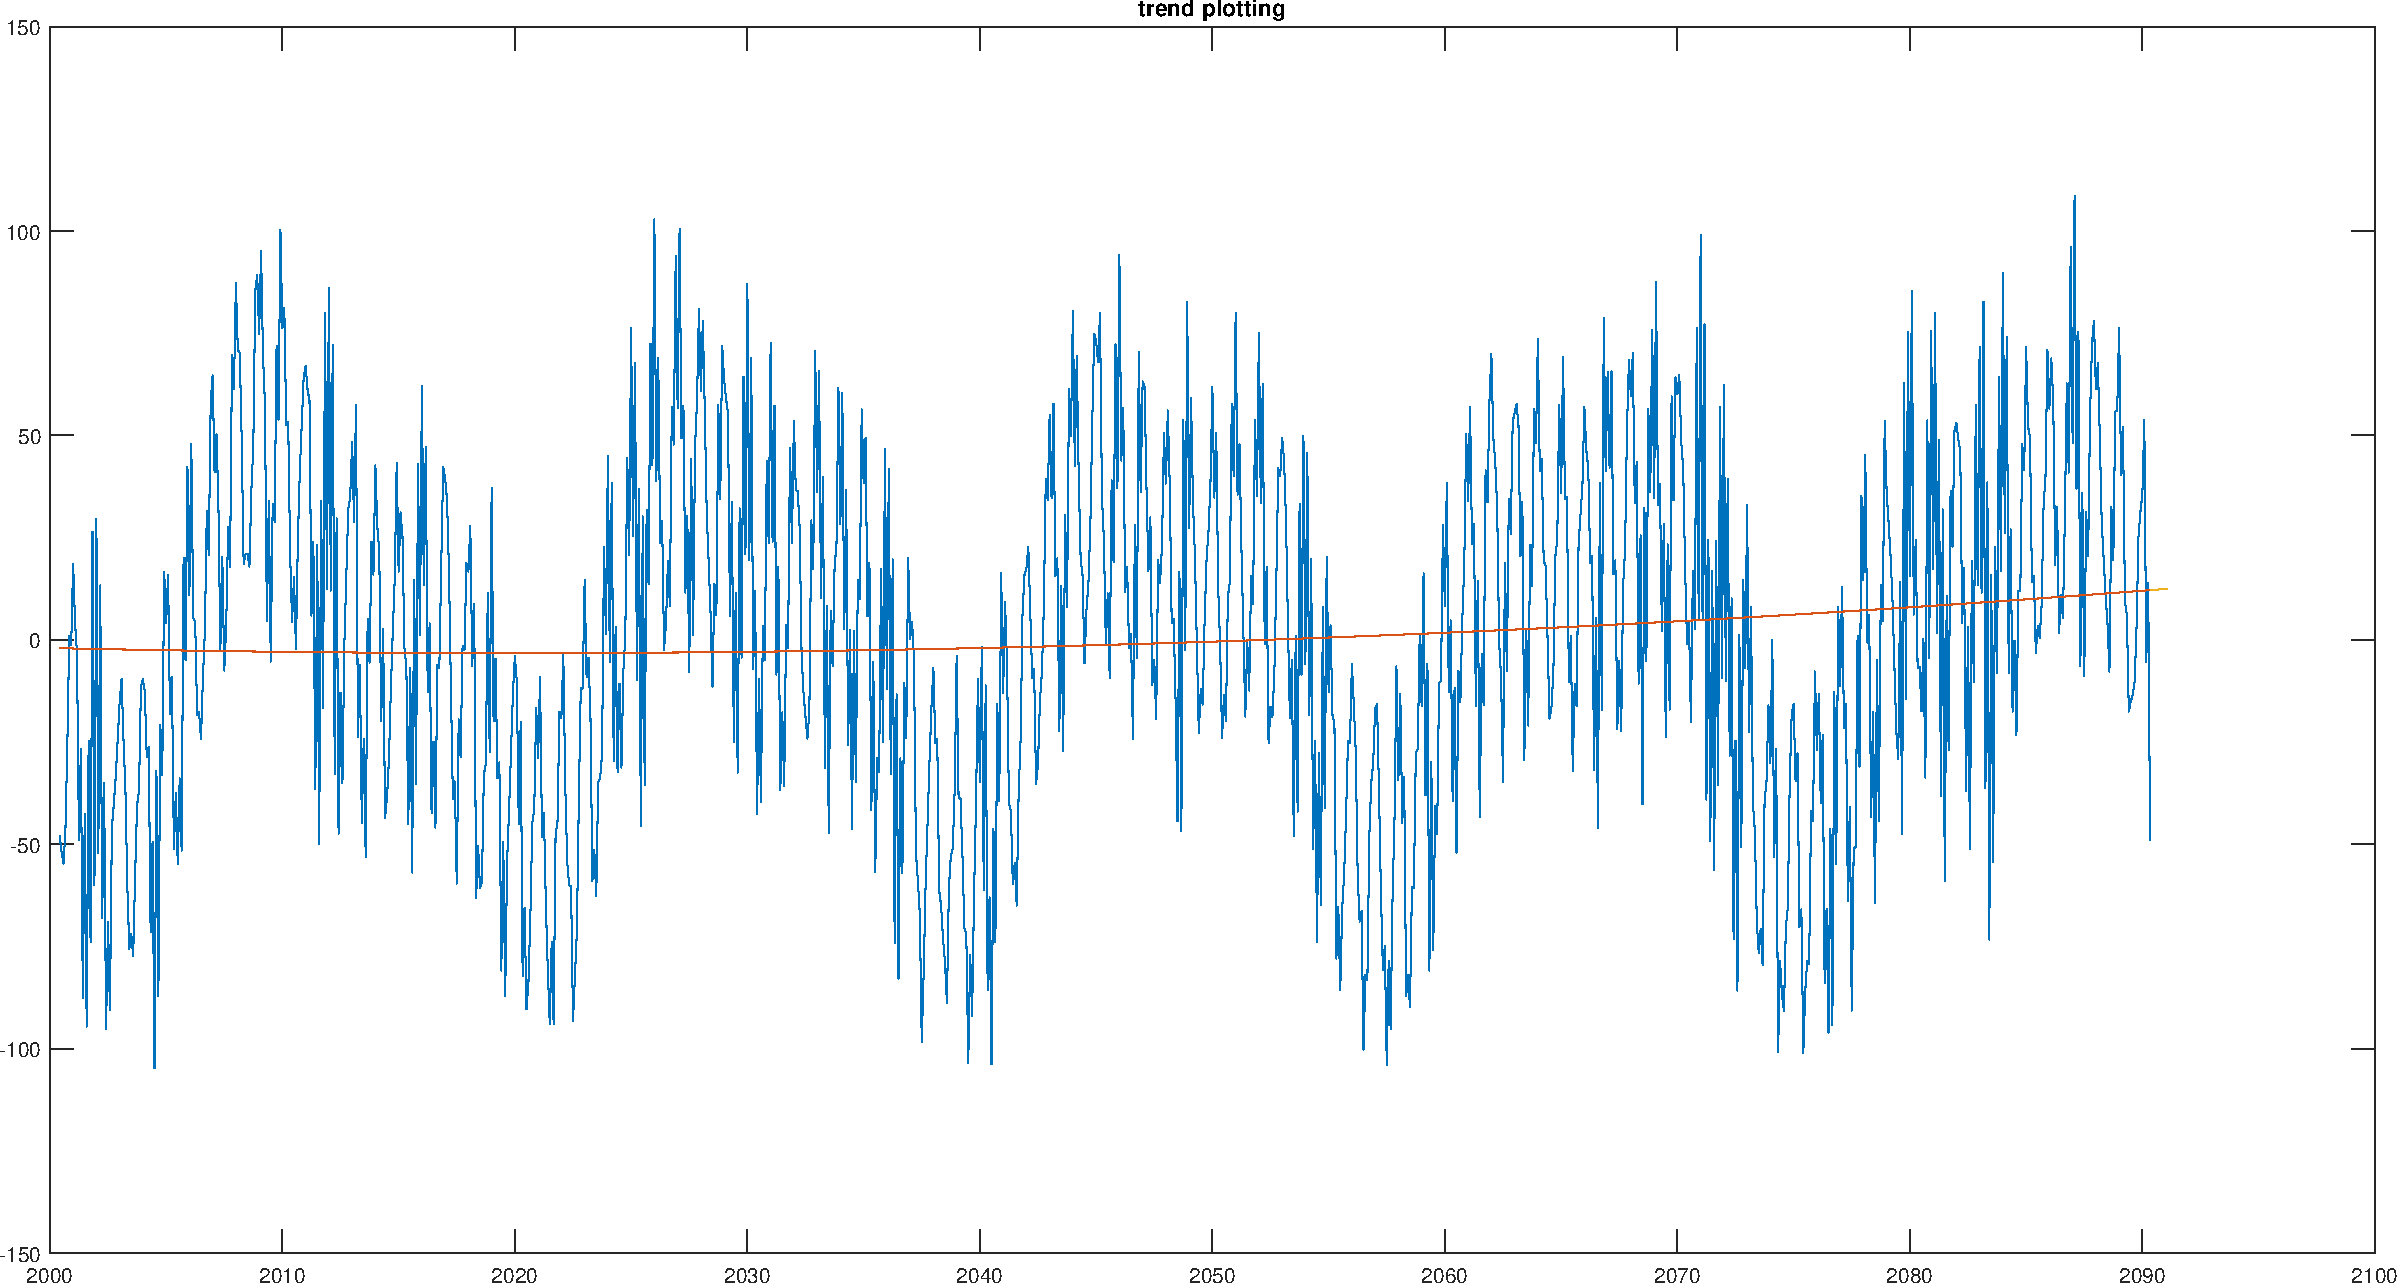
\includegraphics[width=1\linewidth]{inc/task3_predict_poly}}
	\caption{Тренд}
	\label{task3_predict_poly}
\end{figure}

Подберем гармоники задав периоды 1, 8.86 и 18.6 лет (рис. \ref{task3_predict_harm}-\ref{task3_del_harm}):
\begin{figure}[!h]
	\center{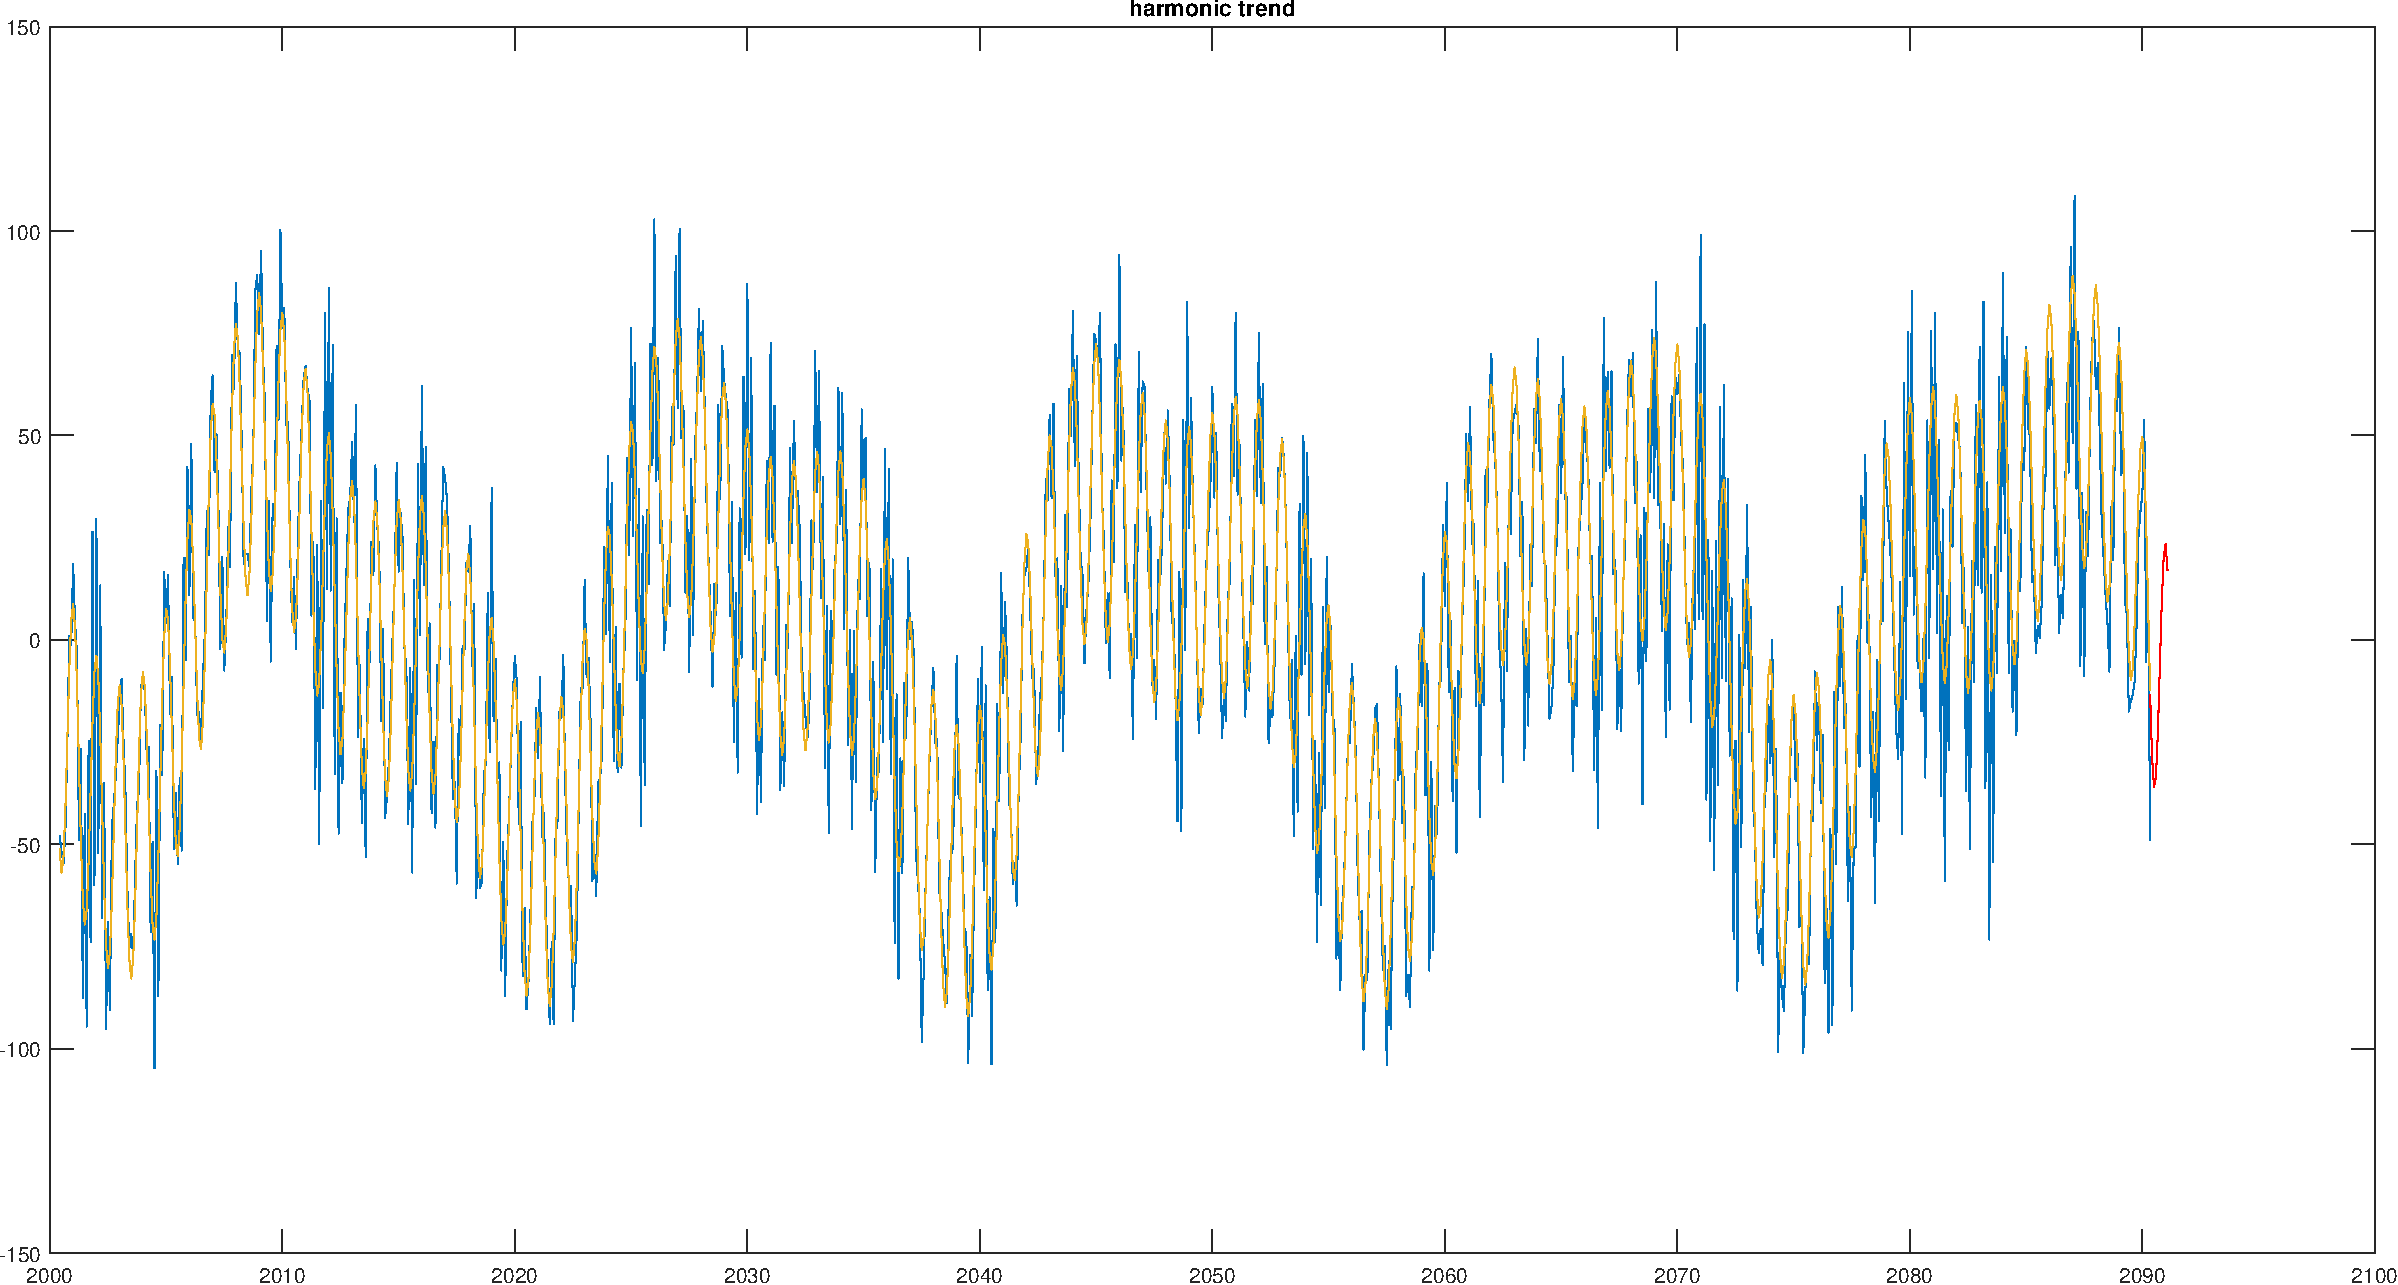
\includegraphics[width=1\linewidth]{inc/task3_predict_harm}}
	\caption{Тренд гармоник}
	\label{task3_predict_harm}
\end{figure}

\newpage
\begin{figure}[!h]
	\center{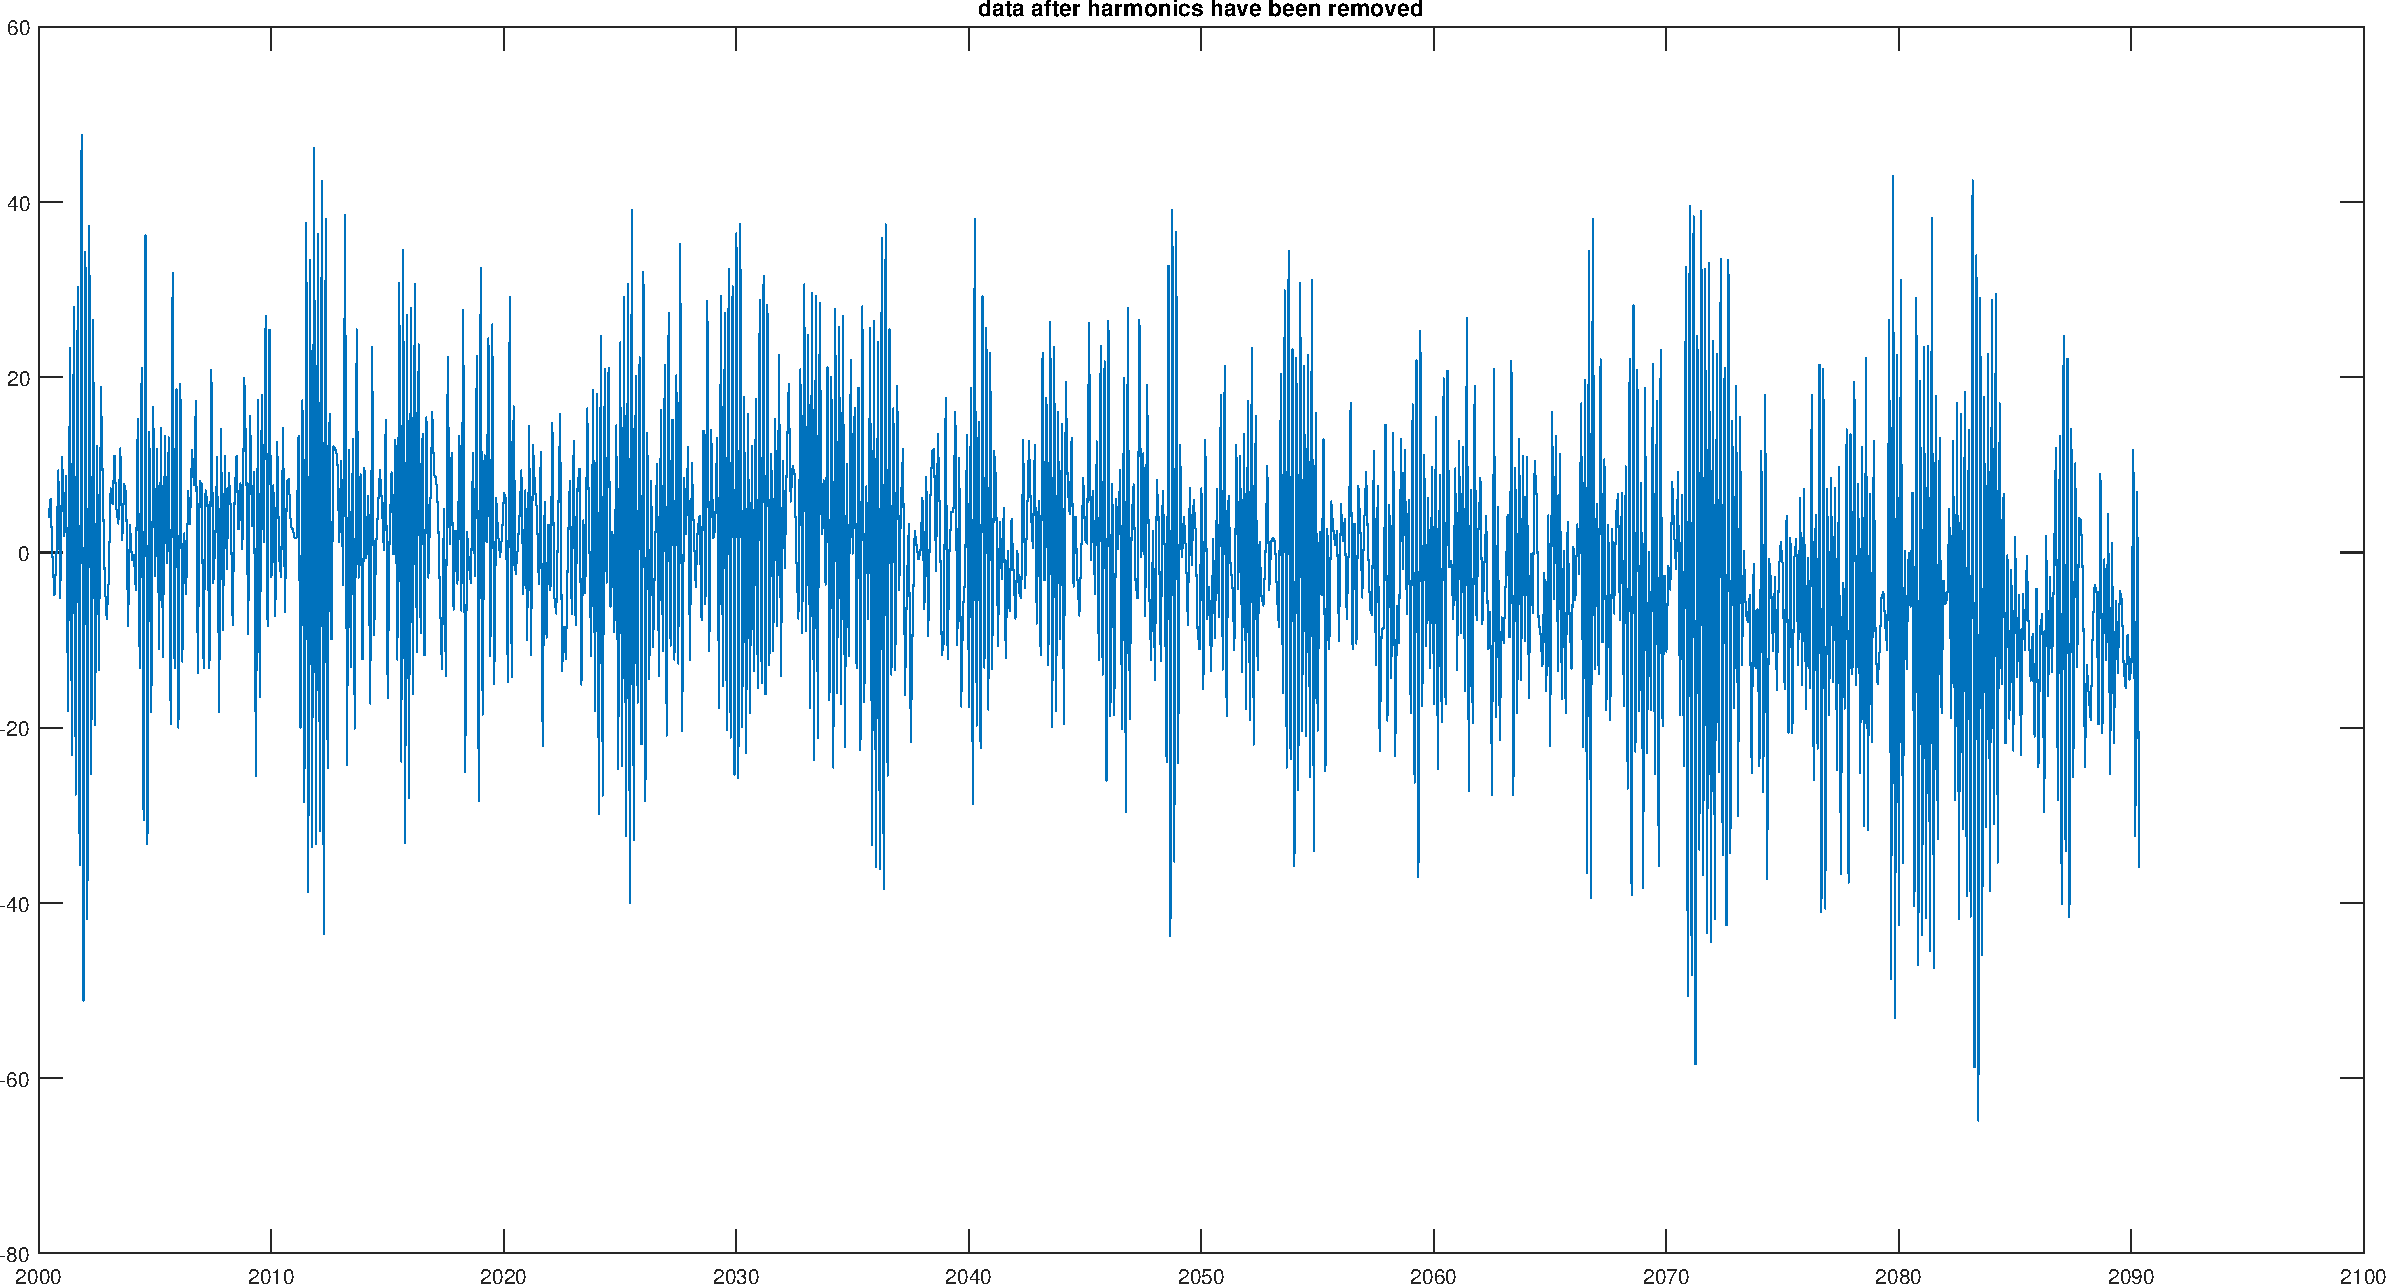
\includegraphics[width=1\linewidth]{inc/task3_del_harm}}
	\caption{Данные после удаления гармоник}
	\label{task3_del_harm}
\end{figure}

Подберем авторегрессию, возьмем порядок 50 (рис. \ref{task3_predict_ar50}):
\begin{figure}[!h]
	\center{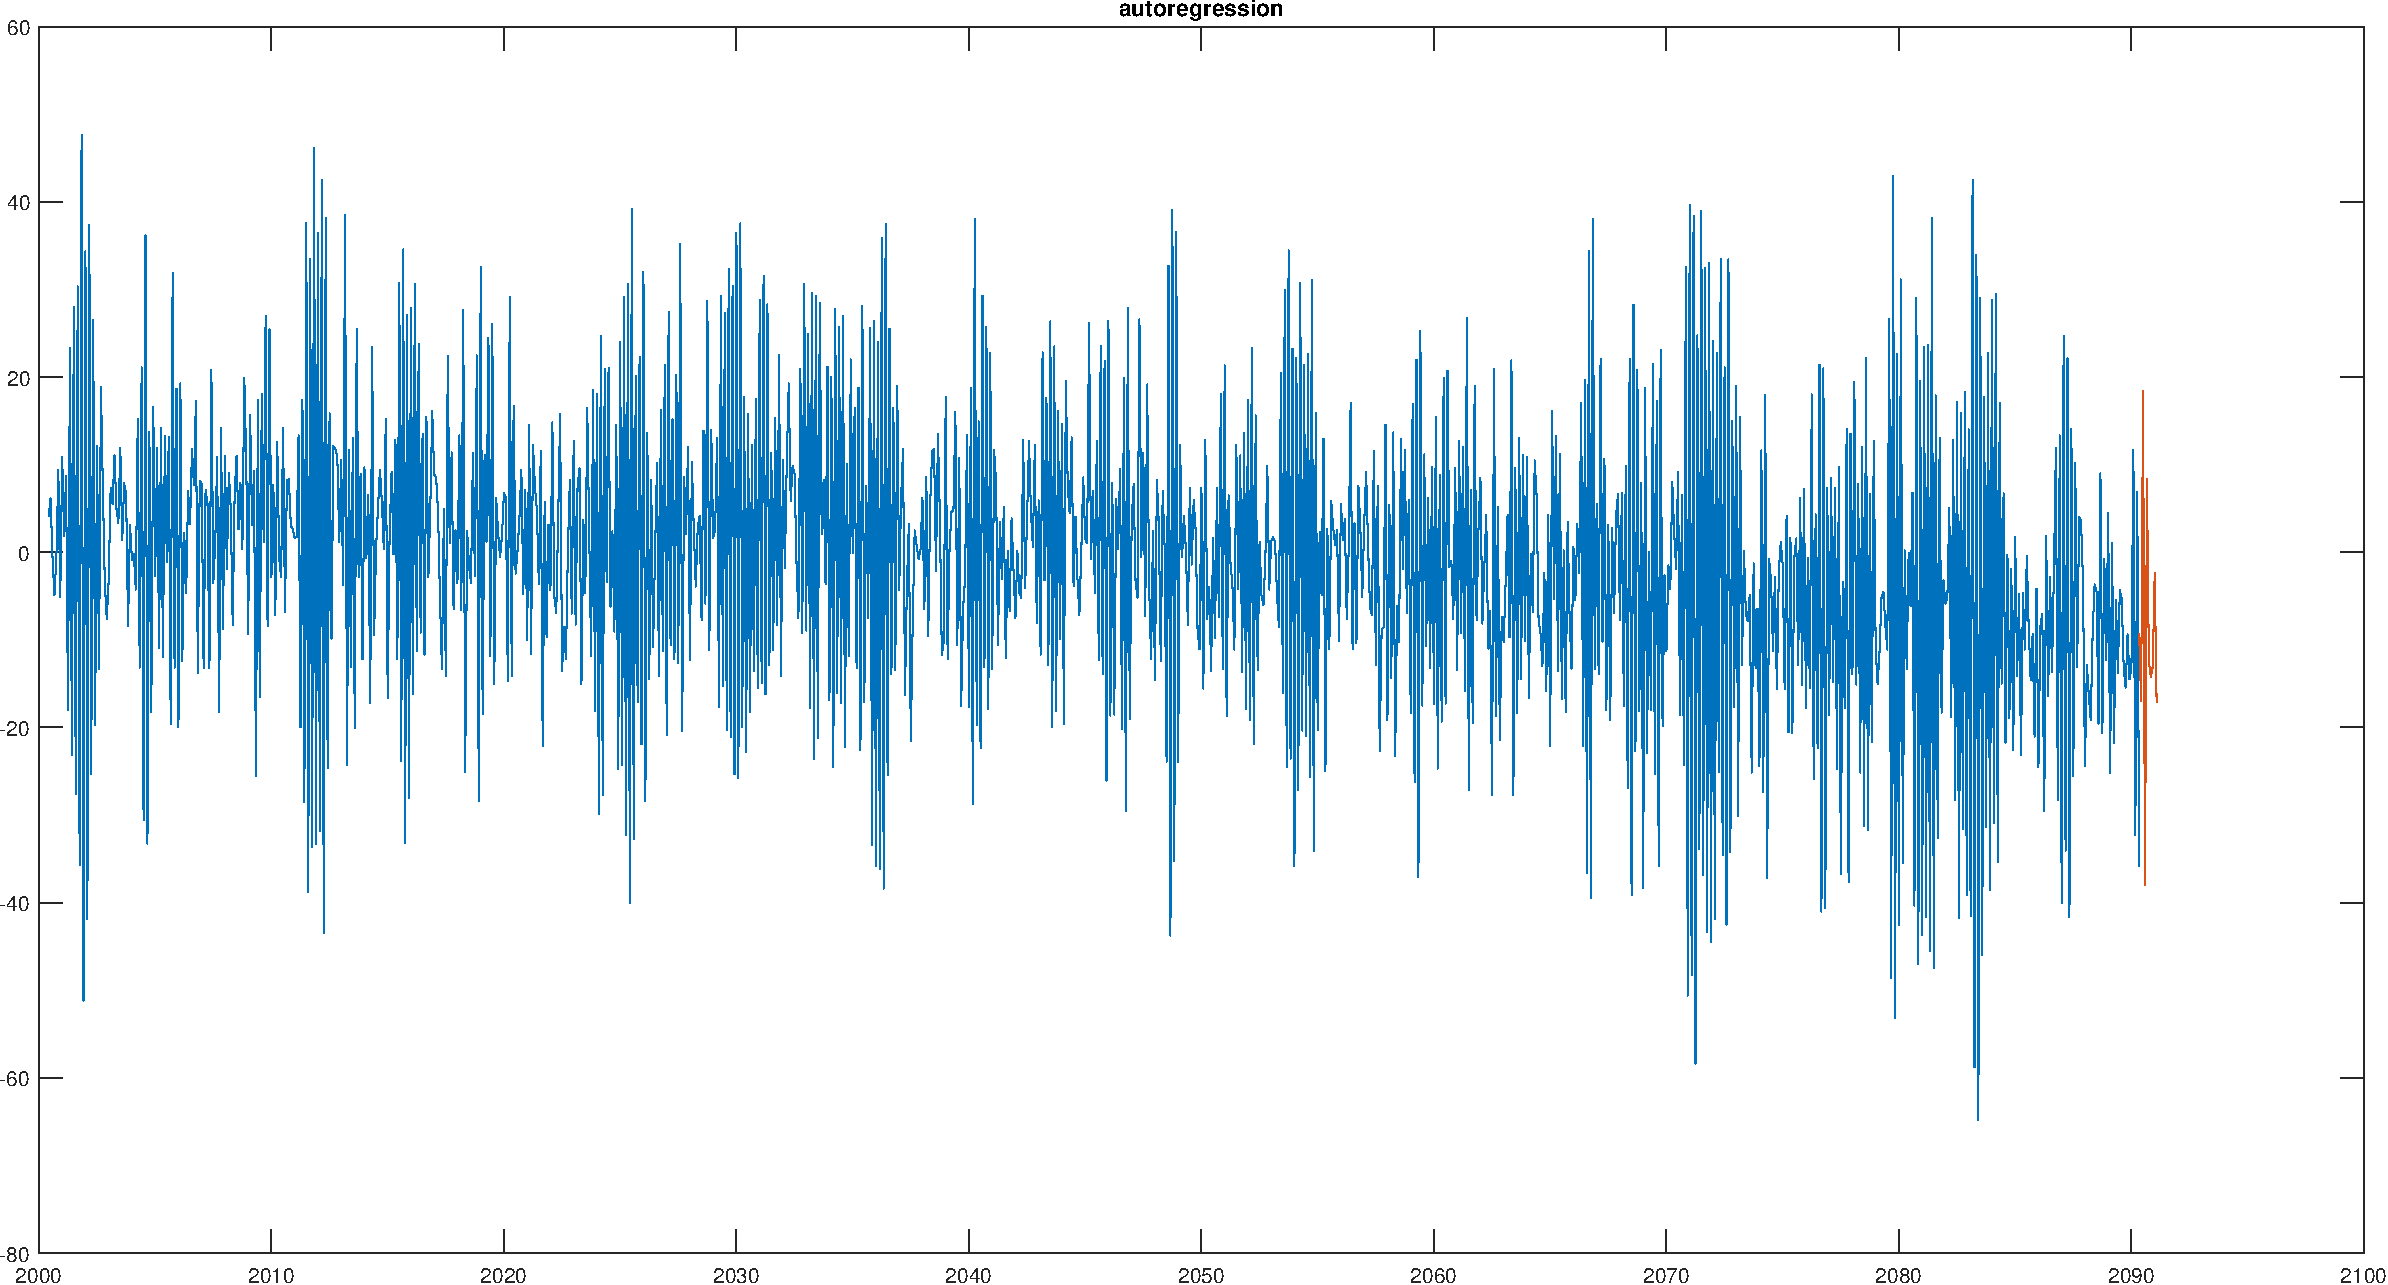
\includegraphics[width=1\linewidth]{inc/task3_predict_ar50}}
	\caption{Авторегрессия с порядком = 50}
	\label{task3_predict_ar50}
\end{figure}

\newpage
И наконец построим график прогноза (рис. \ref{task3_predict}):
\begin{figure}[!h]
	\center{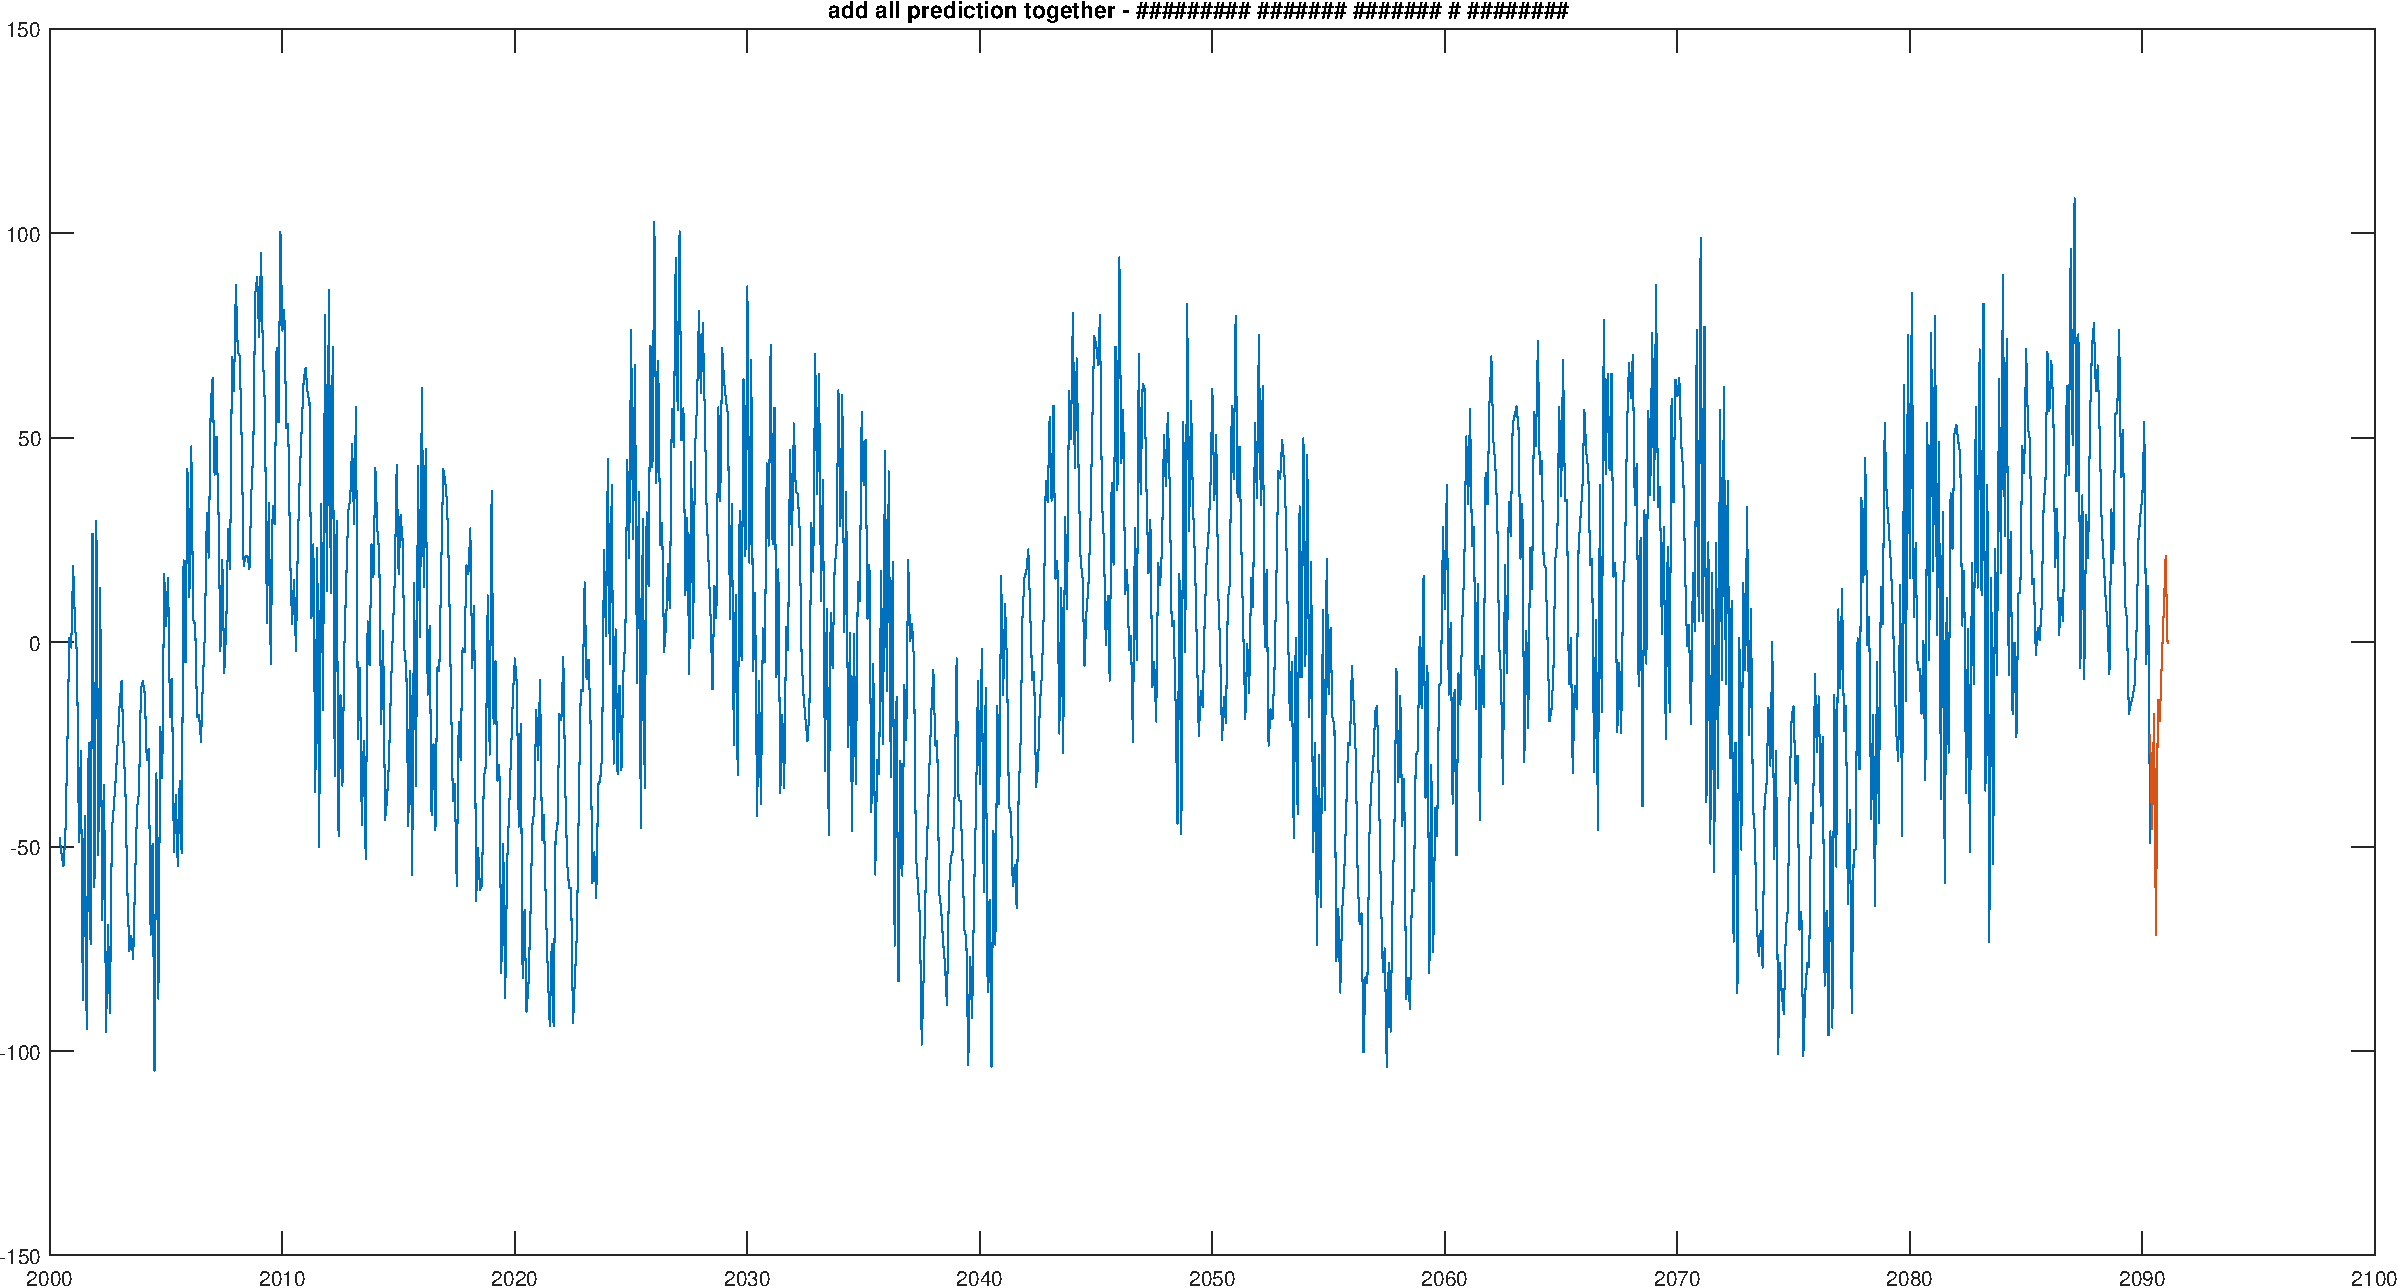
\includegraphics[width=1\linewidth]{inc/task3_predict}}
	\caption{График прогноза}
	\label{task3_predict}
\end{figure}

Можно сравнить прогноз с сигналом и авторегрессией продолженной на 1 год (рис. \ref{task3_predict_compare}):
\begin{figure}[!h]
	\center{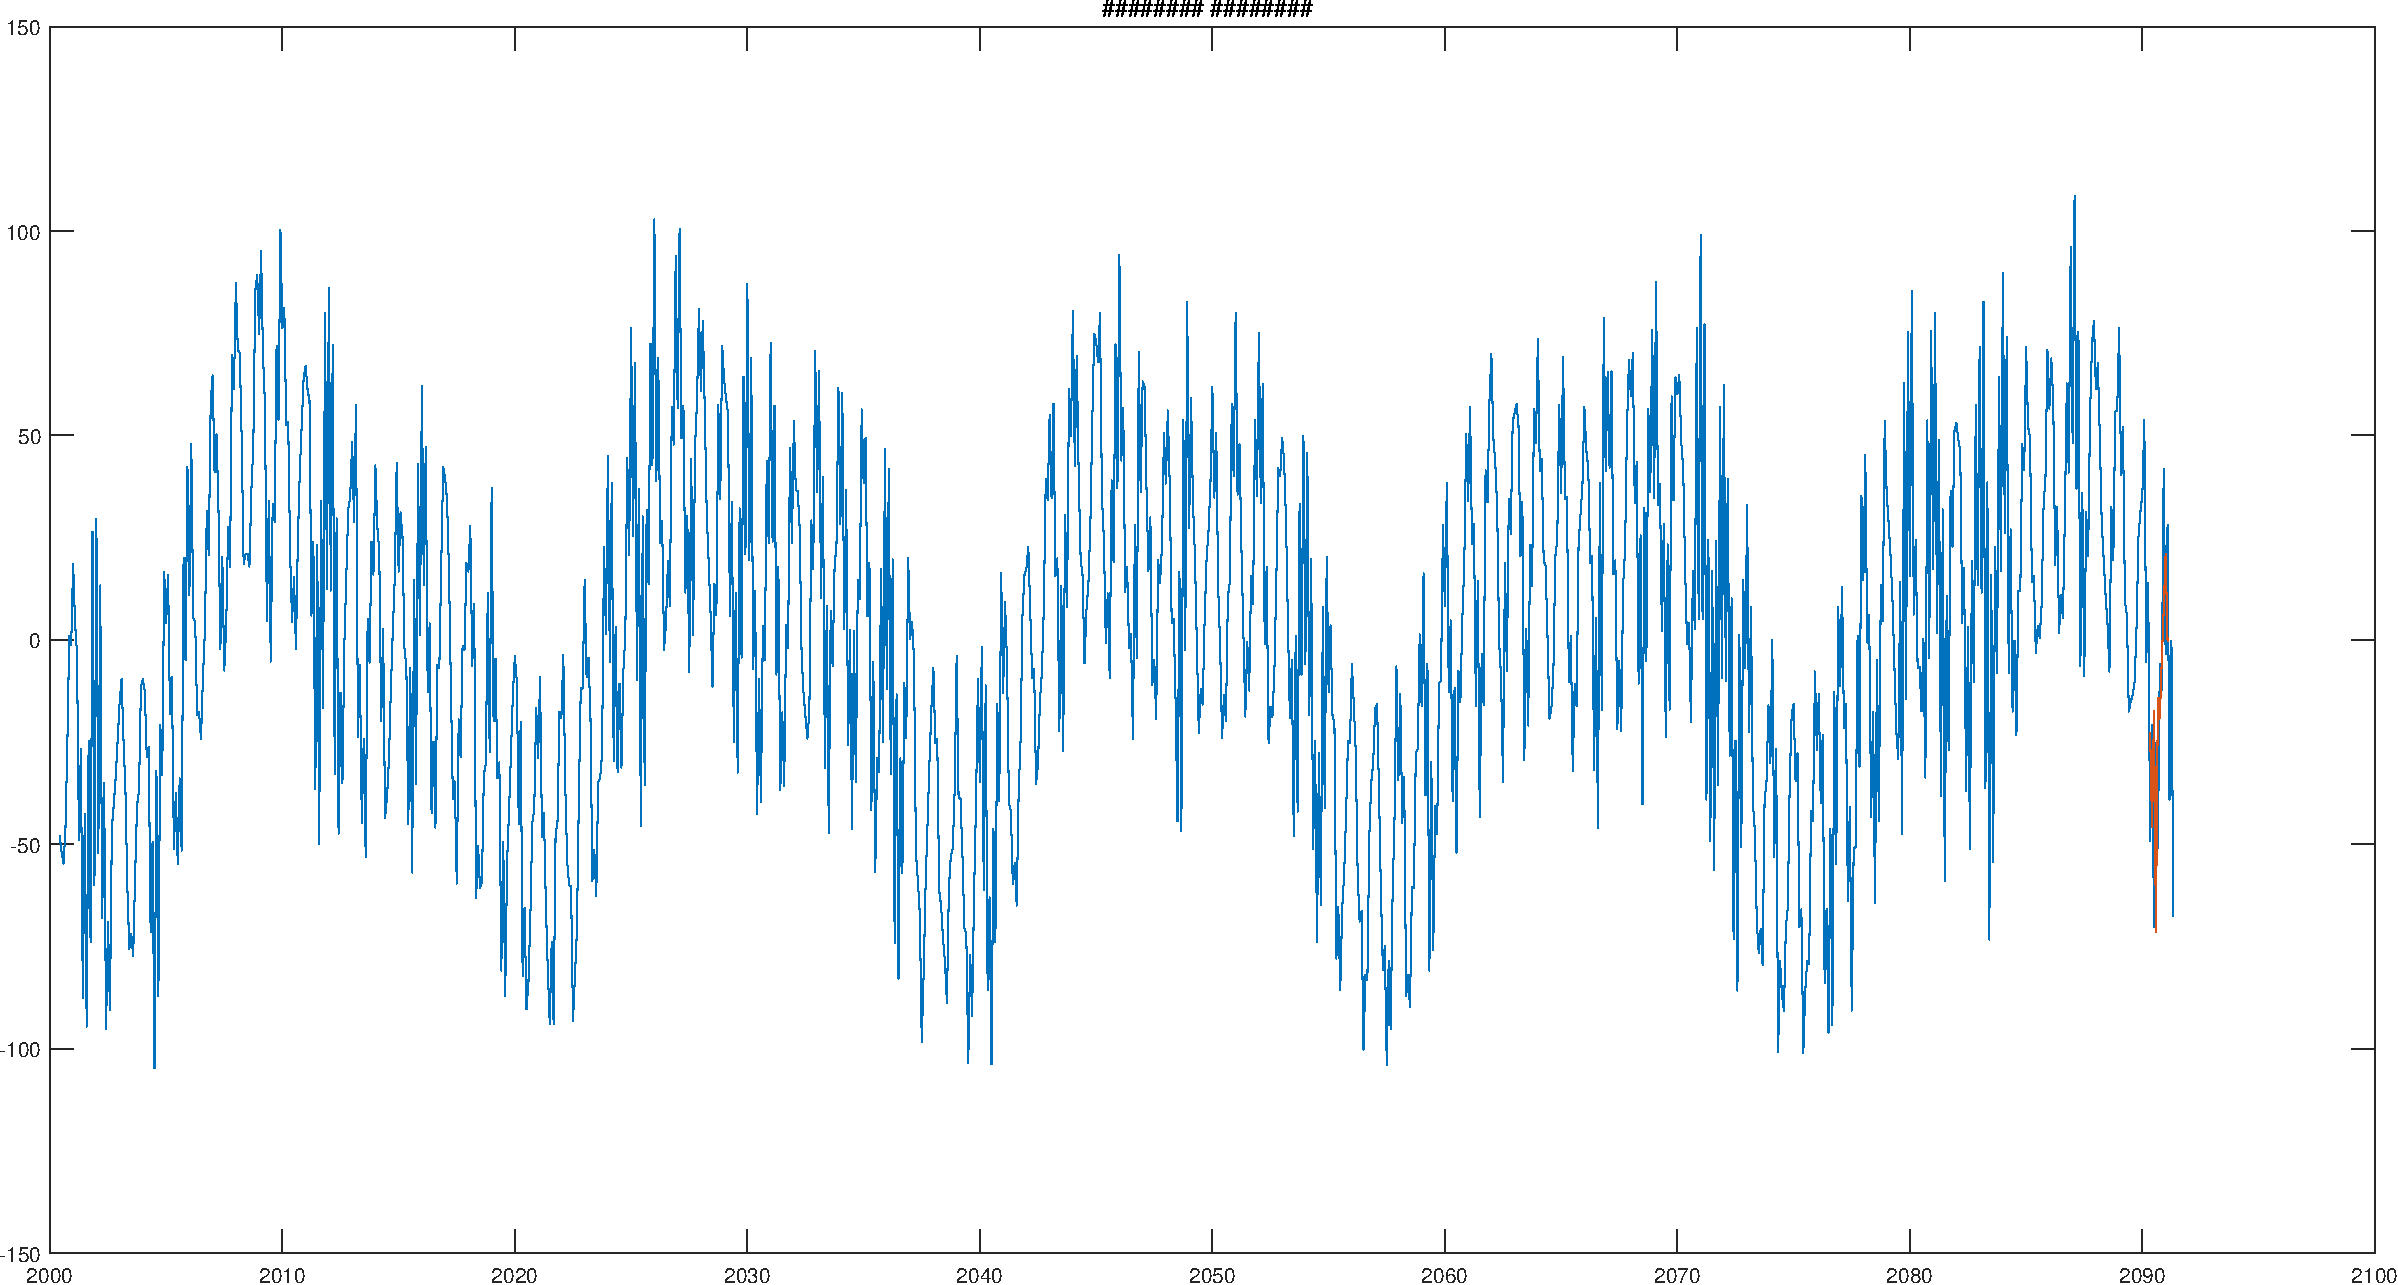
\includegraphics[width=1\linewidth]{inc/task3_predict_compare}}
	\caption{Сравнение прогноза с продолженным сигналом}
	\label{task3_predict_compare}
\end{figure}

Как видно по графику \ref{task3_predict_compare} предсказание в принципе ухватывает общую тенденцию изменения сигнала.

\section*{Исправления}
Увеличим период предсказывания до 20 лет (рис. \ref{task3_predict_compare2}-\ref{task3_predict_compare3})

\begin{figure}[!h]
	\center{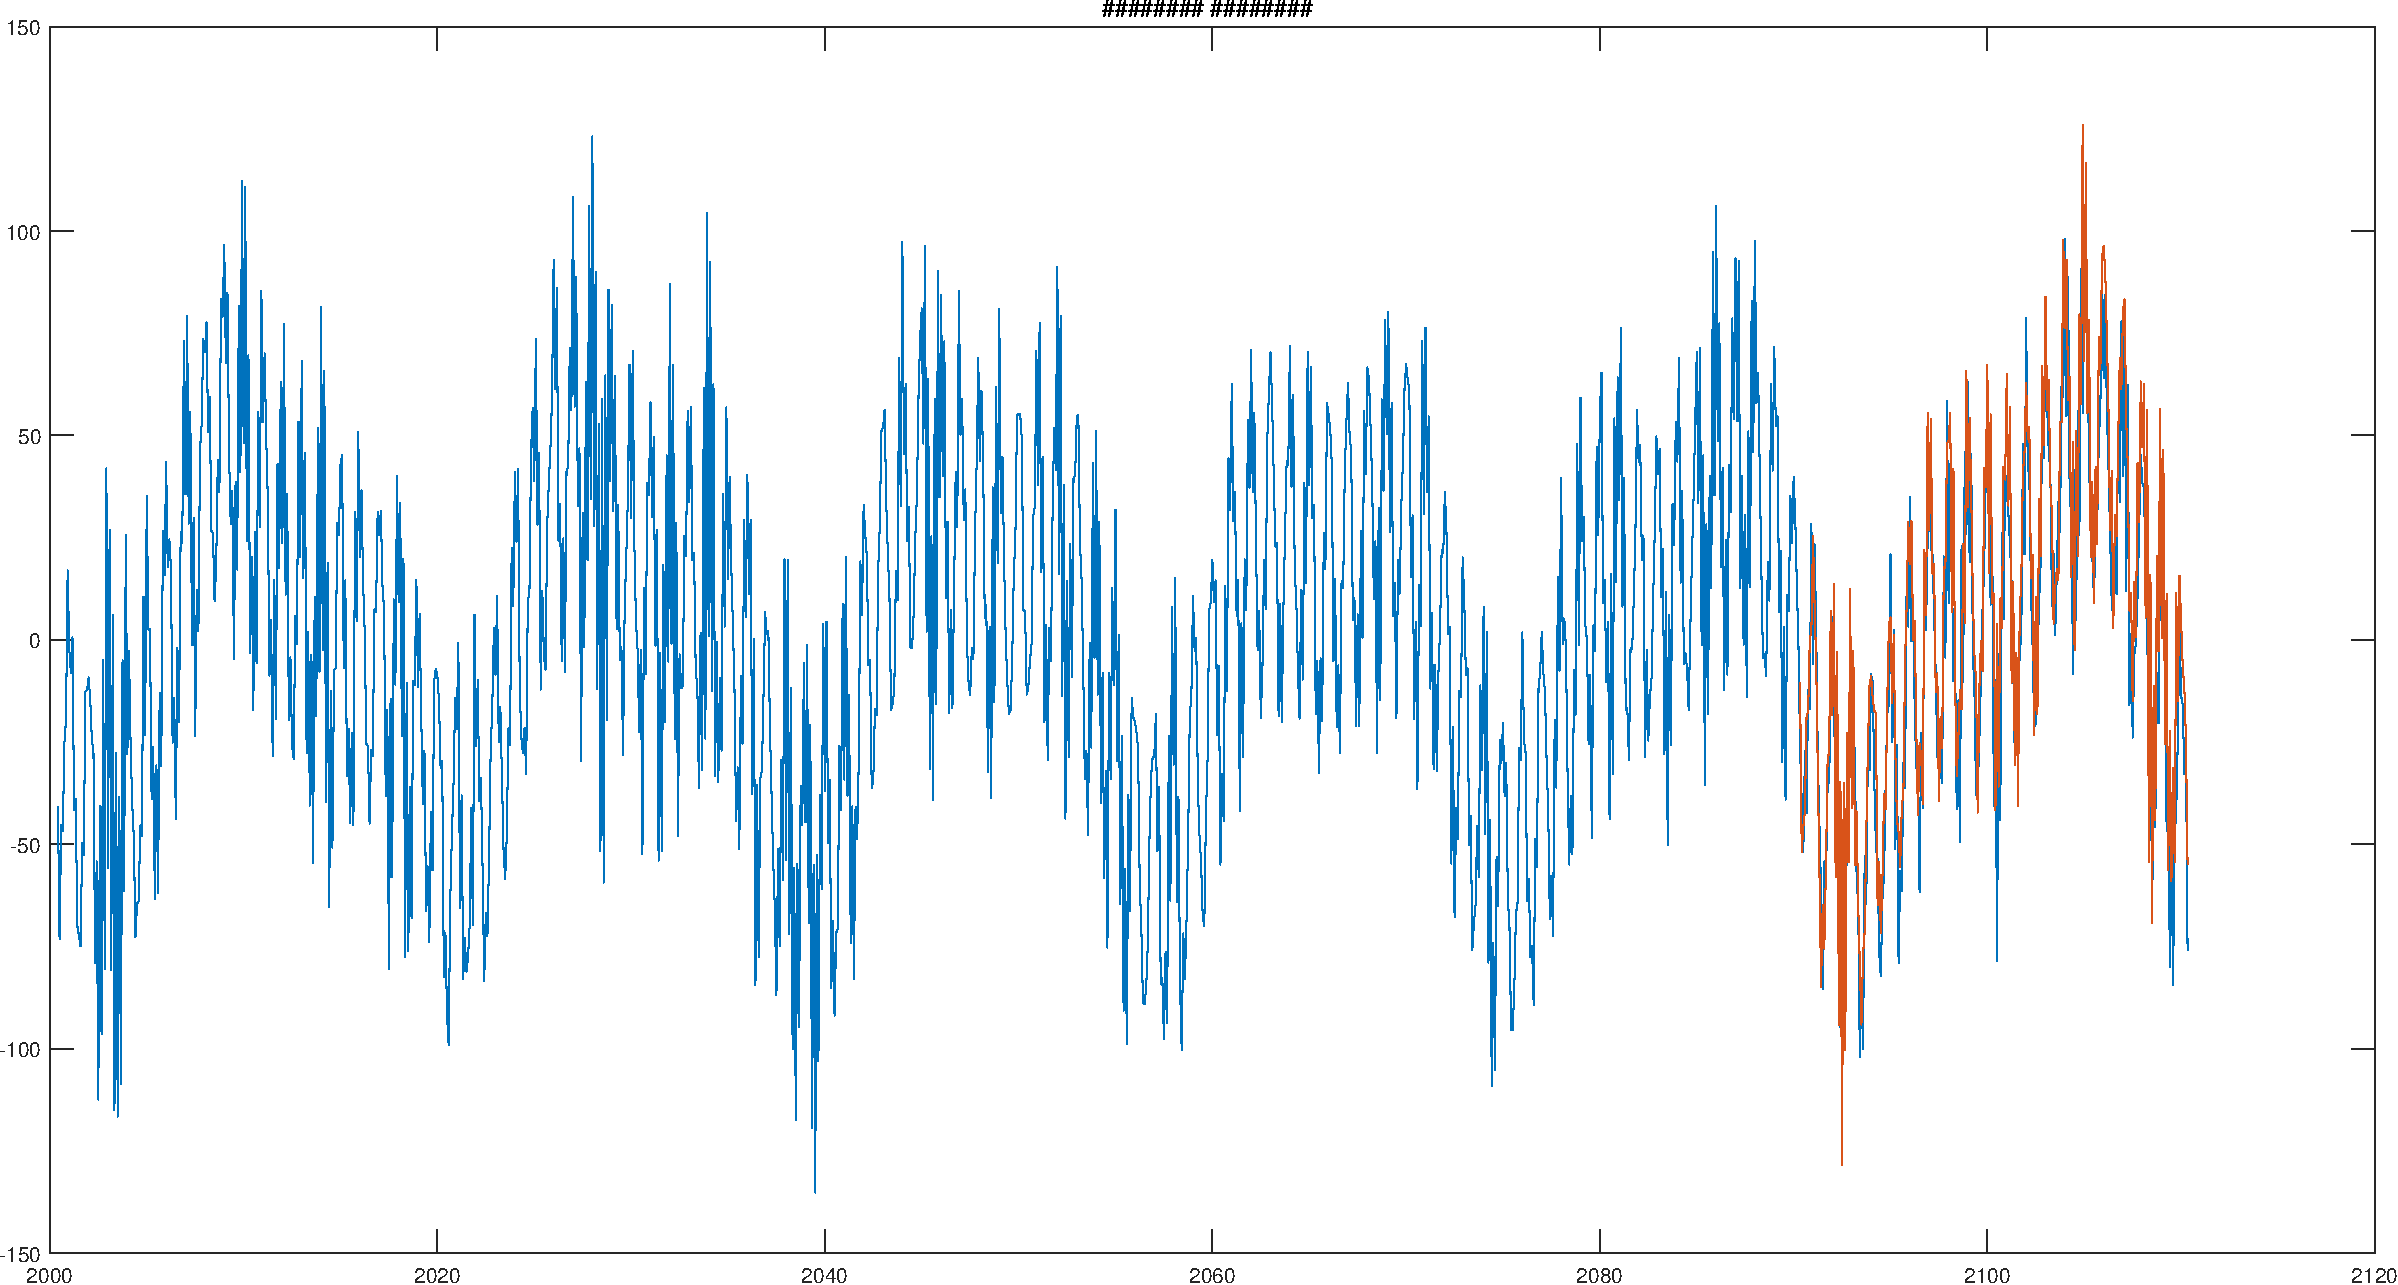
\includegraphics[width=1\linewidth]{inc/task3_predict_compare2}}
	\caption{Сравнение прогноза на 20 лет с продолженным сигналом 1}
	\label{task3_predict_compare2}
\end{figure}

\begin{figure}[!h]
\center{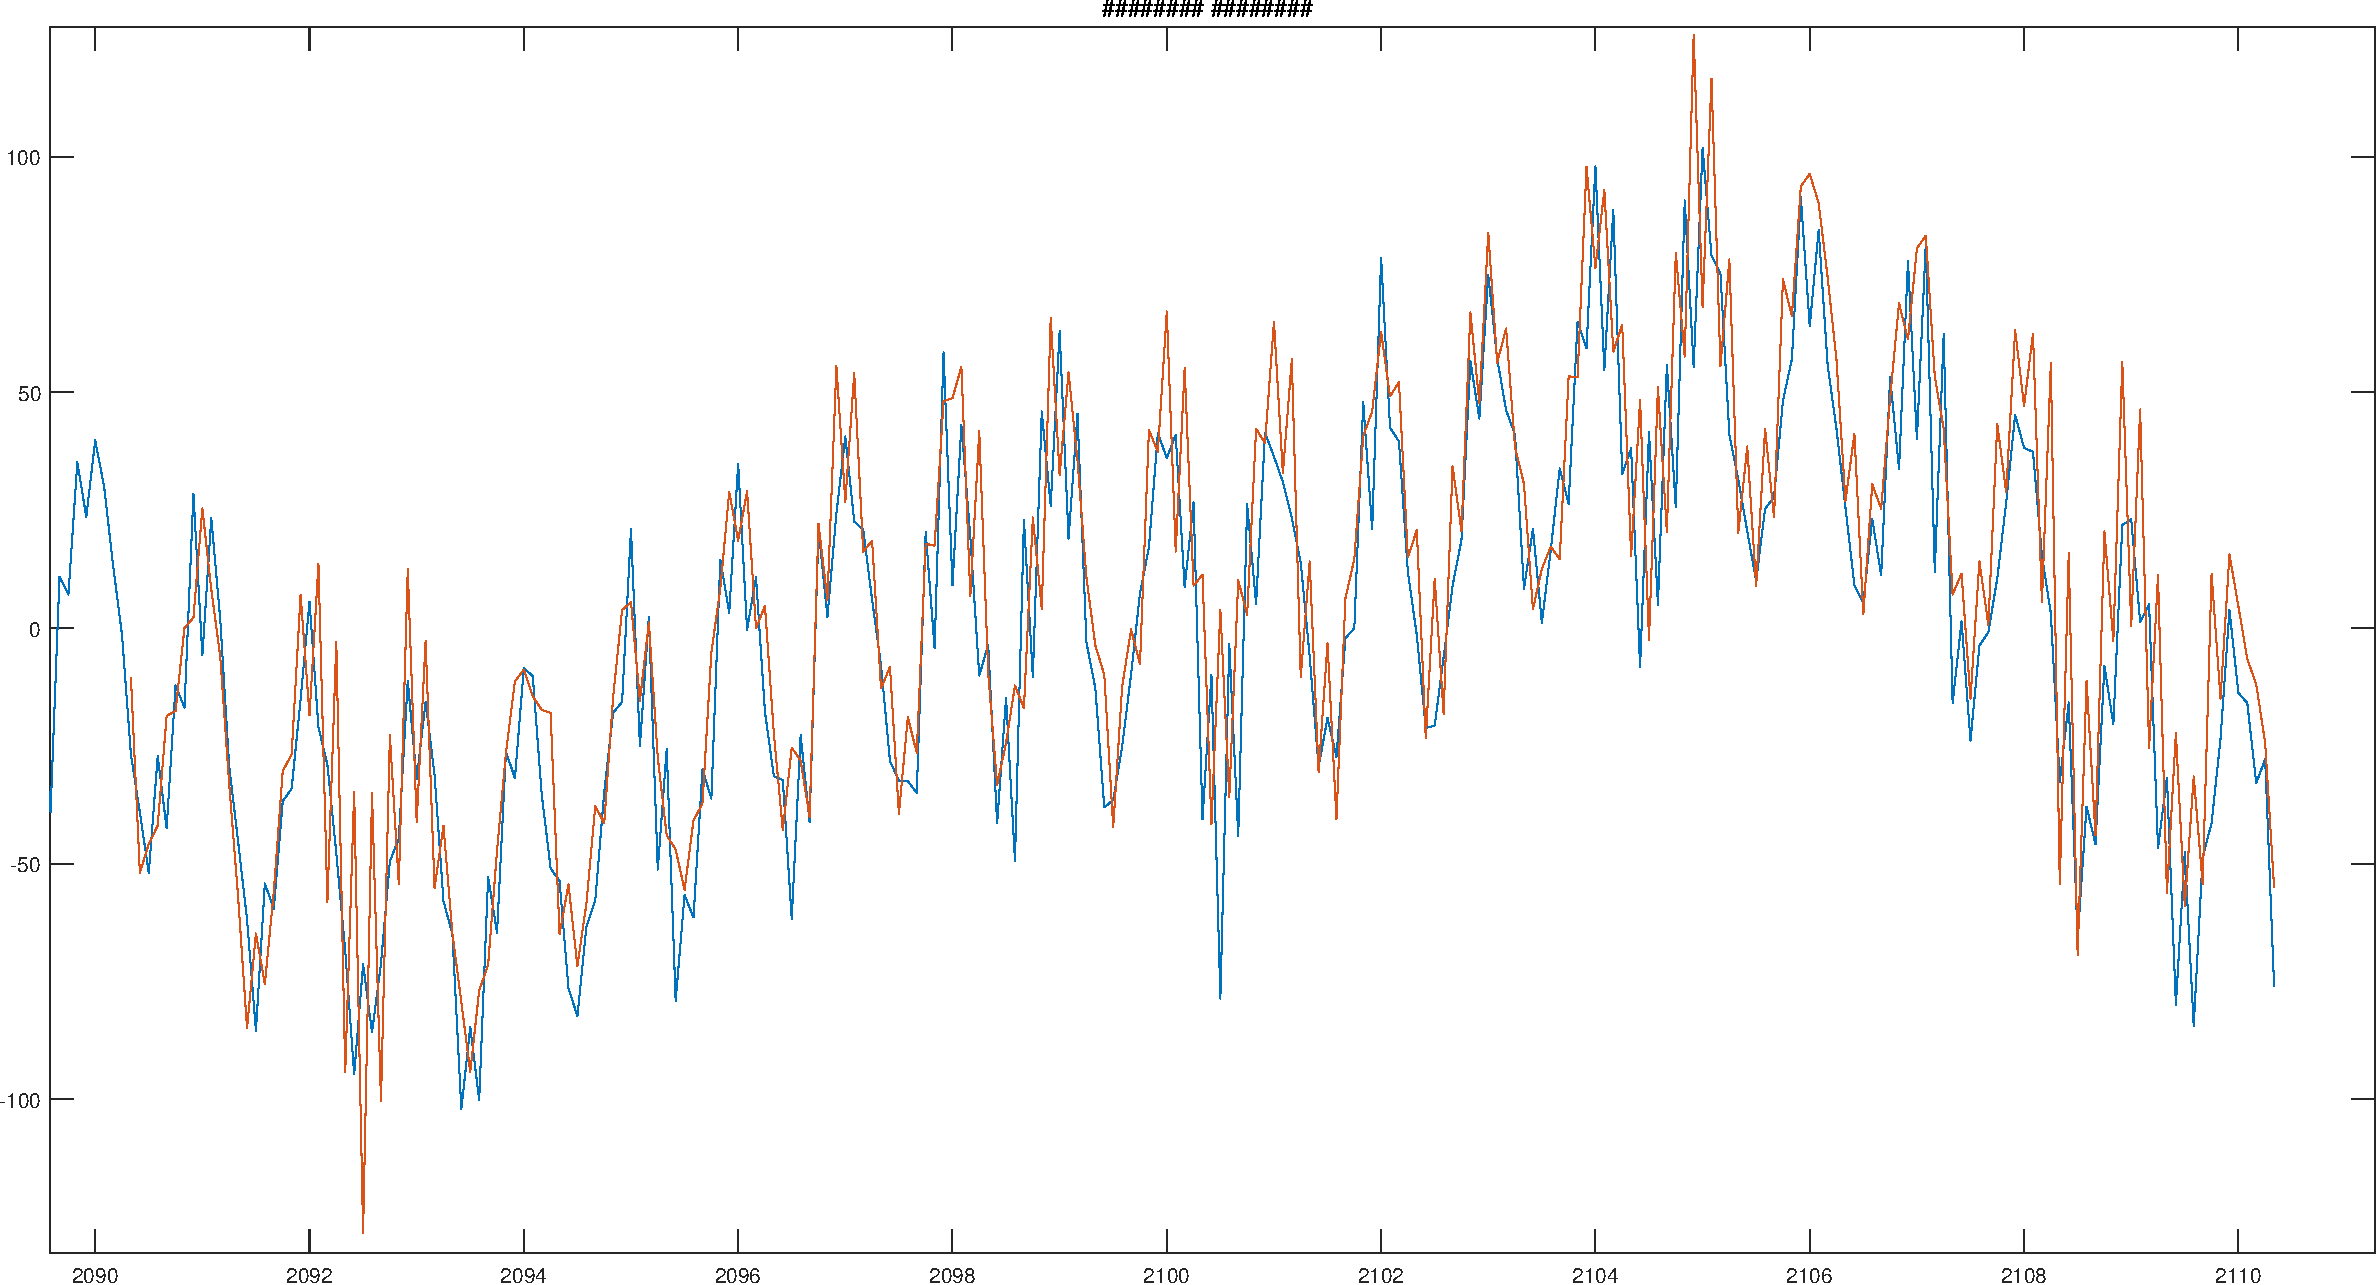
\includegraphics[width=1\linewidth]{inc/task3_predict_compare3}}
\caption{Сравнение прогноза на 20 лет с продолженным сигналом 2}
\label{task3_predict_compare3}
\end{figure}

Как видно из графиков \ref{task3_predict_compare2}-\ref{task3_predict_compare3}, прогноз схож с реальным сигналом.

\end{document}